%!TEX TS-program = latex
\documentclass[12pt]{amsbook}
\usepackage{amssymb, amsmath,latexsym,layout, graphics,color}
\usepackage{amssymb,epsfig}
\usepackage {amsmath}
\usepackage {amsthm}
\usepackage {epsf}
\usepackage{tikz, pgfplots, caption}
\usepackage{enumerate}
\usepackage{multirow}


\usetikzlibrary{arrows,decorations.pathmorphing,backgrounds,positioning,fit,petri}

%\pgfplotsset{axis lines=middle, }

%\setlength{\topmargin}{-.5in}
\setlength{\textheight}{8.5in}
\setlength{\oddsidemargin}{.15in}
%\setlength{\evensidemargin}{-.3in}
\setlength{\textwidth}{6in}
%\setcounter{secnumdepth}{5}
%\setcounter{tocdepth}{5}
\pagestyle{myheadings}


\theoremstyle{definition}
\newtheorem{theorem}{Theorem}
\newtheorem{definition}{Definition}[section]
\newtheorem{xca}{Exercise}[section]

\usepackage{chngcntr}
\counterwithin{table}{section}

\title[Introduction to Game Theory]%
{Introduction to Game Theory:
 a Discovery Approach}
 \author{Jennifer Firkins Nordstrom}
 
 %Be sure to run makeindex <filename.idx>

\makeindex

\begin{document}
\frontmatter
\maketitle
\tableofcontents
\include{Preface}
\mainmatter

% Master file for IGT

\chapter{What is Game Theory?}

\vspace{.2in}
``Game Theory is not about `playing games.' It is about conflict resolution among rational but distrustful beings.'' Poundstone, {\it Prisoner's Dilemma}, p. 39.

Although we will play lots of games in throughout this book, our goal is to understand how rational, distrustful players would play the game. We will explore how to behave as such players, and how to ``solve'' games under certain assumptions about our players.

\vspace{.1in}

\section{Players and Strategies}\label{S:intro}

In this book most of the games will be played by two \emph{players}\index{player}. Each player must decide how he or she will play the game. In order to study games mathematically, we need to make some assumptions about how the players should play the game. This allows us to be able to better predict what our players should do. The following example illustrates the characteristics we will assume about our players.


\subsection{Example: Cake Division}\label{Ex:Cake}\index{Cake Division}



How can two children fairly divide a cake? One classic solution is to have one child cut the cake and have the other child choose a piece.

Why does this work? In other words, why should both children feel they received a fair share of the cake?

What are the underlying assumptions that make this process work?
\begin{enumerate}
\item The goal of each player is to get the largest piece. We can think of this as each player acting in his or her \emph{self-interest}\index{self-interest}.
\item Both players know that the other player has the same goal, and will act to further this goal. Thus, we know that each player is \emph{rational}\index{rational} Even more, each player knows the \emph{other} player is rational.
\end{enumerate}

We need both (1) and (2) to reach the solution that the cake is divided evenly and both children receive equal sized pieces.

The idea that players are self-interested is crucial to game theory. There are lots of other ways to play games, and those might be worth exploring. But to get started with game theory, we must make specific assumptions and develop the mathematical context from these assumptions. 

%\subsection{Understanding the Assumptions}

{\bf Assumption 1:}\index{assumptions} Players are self-interested. The goal is to win the most or lose the least. What does it mean to win? 

A player's \emph{payoff}\index{payoff} is the amount (points, money, or anything a player values) a player receives for a particular outcome of a game. We say that the player's goal is to maximize his or her payoff. We should note that the maximum payoff for a player might even be negative, in which case the player wants the least negative (or closest to 0) payoff.

It is important to recognize the difference between having the goal of maximizing the payoff and having the goal of simply winning. Here are some examples.
\begin{enumerate}
\item If two players were racing, a player wouldn't just want to finish first, she would want to finish by as large a margin as possible.
\item If two teams were playing basketball, the team wouldn't want to just have the higher score, they would want to win by the largest number of points. In other words, a team would prefer to win by 10 points rather than by 1 point.
\item In an election poll, a candidate doesn't just want to be ahead of her opponent, she wants lead by as large a margin as possible, (especially if she needs to account for error in the polls).
\end{enumerate}

It is important to keep in mind the the goal of each player is to win the most (or lose the least). It will be tempting to look for strategies which simply assure a player of a positive payoff, but we need to make sure a player can't do even better with a different strategy. 

{\bf Assumption 2:}\index{assumptions}  Players are perfectly logical. Players will always take into account all available information and make the decision which maximizes his payoff. This includes knowing that his opponent is also making the best decision for herself. 
For example, in the cake cutting game a player wouldn't cut one large piece hoping that his opponent will by chance pick the smaller piece. A player must assume that her opponent will always choose the larger piece.

Now you may be wondering what these assumptions have to do with reality. After all, no one's perfect. But we often study ideal situations (especially in math!). For example, you've all studied geometry. Can anyone here draw a perfectly straight line? Yet you've all studied such an object!


{\bf Our Goal: Develop strategies for our perfectly logical, self-interested players.}

\subsection{Developing Strategies: Tic Tac Toe}\label{Ex:Tic}\index{Tic Tac Toe }

%\begin{enumerate}
\begin{xca} Play several games of Tic TacToe with an opponent. Make sure you take turns being the first player and the second player. Develop a strategy for winning Tic Tac Toe. You may have a different strategy for the first player and for the second player. Be as specific as possible. You may need to consider several possibilities which depend on what the opponent does.

\begin{enumerate}[(a)]
\item Who wins? Player 1 or Player 2?
\item What must each player do in order to have the best possible outcome?
\item How did you develop your strategy?
\item How do you know it will always work?
\end{enumerate}
\end{xca}
 
%\end{enumerate}

Let us note some characteristics of Tic Tac Toe.
\begin{itemize}
\item There are two players.
\item Players have {\it perfect information}\index{perfect information}. This means each player knows what all of his or her own options are, what all of his or her opponent's options are, and both players know what the outcome of each option is. Additionally, players know that both players have all of this information.

\item This game has a {\it solution}\index{solution}.  A solution for a game consists of a strategy for each player and the outcome of the game when each player plays his or her strategy. In Tic Tac Toe, if both players play their best, the game will always end in a tie.
\item The game is {\it finite}\index{finite game}. This means the game must end after a finite number of moves of turns. In other words, the game cannot go on forever. A game that is not finite is called \emph{infinite}\index{infinite game}. Note, an infinite game may end after a finite number of turns, but there is no maximum number of turns or process to ensure the game ends. In Tic Tac Toe, the game must end after 9 or fewer turns. 
\end{itemize}

\begin{xca}
Can you think of another  example of a game with perfect information? What is an example of a game that does not have perfect information?
\end{xca}

\begin{xca}
Give some examples of finite games and infinite games.
\end{xca}


\begin{definition} A  \emph{strategy} for a player is a complete way to play the game regardless of what the other player does. 
\end{definition}

The choice of what a player does may depend on the opponent, but that choice is predetermined before game play. For example, in the cake cutting game, it doesn't matter which piece the ``chooser'' will pick, the ``cutter'' will always cut evenly. Similarly, it doesn't matter how the cutter cuts, the chooser will always pick the largest piece. In tic-tac-toe, Player 2's strategy should determine his first move no matter what Player 1 plays first. For  example, if Player 1 plays the center square, where should Player 2 play? If Player 1 plays a corner, where should Player 2 play?    

%\begin{enumerate}
%\setcounter{enumi}{1}
%\item Earlier you developed a solution for TIC-TAC-TOE. Write up the complete solution for TIC-TAC-TOE. Your solution should include strategies for each player and the outcome of the game. You may include charts or tables if they will help clarify your solution, but you should have a complete written solution as well.

\vspace{.1in}

\begin{xca}What is your favorite game?
\begin{enumerate}[(a)]
\item Give a brief description of the game, including what it means to ``win'' or ``lose'' the game.

\item How many players do you need?

\item Do the players have perfect information for the game?

\item Is the game finite or can it go on forever?

\item Give some possible strategies for the player(s). Note, depending on the game, these strategies may not always result in a definite win, but they should suggest a way to increase a player's chances of winning (or not losing).

\end{enumerate}


\end{xca}




%\input{IntroductionB}

\section{Game Matrices and Payoff Vectors}

%\markright{Game Matrices}

\vspace{.2in}

We need a way to describe the possible choices for the players and the outcomes of those choices.
For now, we will stick with games that have only two players. We will call them Player 1 and Player 2.

\subsection{Example: Matching Pennies}\label{Ex:MatchPennies}\index{Matching Pennies}

Suppose each player has two choices: Heads (H) or Tails (T). If they choose the same letter, then Player 1 wins \$1 from Player 2. If they don't match, then Player 1 loses \$1 to Player 2. We can represent all the possible outcomes of the game with a {\emph{matrix}\index{game matrix}.  

Player 1's options will always correspond to the rows of the matrix, and Player 2's options will correspond to the columns. See Table \ref{T:template}.

%\hspace{1in}Player 2
%\begin{tabular}{l|r|c|c|}\cline{2-4}
%&&\textbf{H}&\textbf{T}\\ \cline{2-4}
%Player 1&\textbf{H} &&\\ \cline{2-4}
%&\textbf{T} &&\\ \cline{2-4}
%\end{tabular}

\begin{table}[h]
\centering

\begin{tabular}{llll}
                      & \multicolumn{3}{l}{Player 2}                                                  \\ \cline{2-4} 
\multicolumn{1}{l|}{} & \multicolumn{1}{l|}{} & \multicolumn{1}{l|}{H} & \multicolumn{1}{l|}{T} \\ \cline{2-4} 
\multicolumn{1}{l|}{Player 1} & \multicolumn{1}{l|}{H} & \multicolumn{1}{l|}{} & \multicolumn{1}{l|}{} \\ \cline{2-4} 
\multicolumn{1}{l|}{} & \multicolumn{1}{l|}{T} & \multicolumn{1}{l|}{} & \multicolumn{1}{l|}{} \\ \cline{2-4} 
\end{tabular}
\caption{A game matrix showing the strategies for each player}
\label{T:template}
\end{table}\medskip

\begin{definition} A \emph{payoff}\index{payoff} is the amount a player receives for  given outcome of the game.\end{definition}

Now we can fill in the matrix with each player's payoff. Since the payoffs to each player are different, we will use ordered pairs where the first number is Player 1's payoff and the second number is Player 2's payoff. The ordered pair is called the \emph{payoff vector}\index{payoff vector}. For example, if both players choose H, then Player 1's payoff is \$1 and Player 2's payoff is -\$1 (since he loses to Player 1). Thus the payoff vector associated with the outcome H, H is $(1, -1)$. 

We fill in the matrix with the appropriate payoff vectors in Table \ref{T:matchpennies}

%\hspace{1.2in}Player 2

%\begin{tabular}{l|r|c|c|}\cline{2-4}
%&&\textbf{A}&\textbf{B}\\ \cline{2-4}
%Player 1&\textbf{A} &(1, -1)&(-1, 1)\\ \cline{2-4}
%&\textbf{B} &(-1, 1)&(1, -1)\\ \cline{2-4}

%\end{tabular}
\begin{table}[h]
\centering

\begin{tabular}{cccc}
                      & \multicolumn{3}{c}{Player 2}                                                  \\ \cline{2-4} 
\multicolumn{1}{l|}{} & \multicolumn{1}{l|}{} & \multicolumn{1}{c|}{H} & \multicolumn{1}{c|}{T} \\ \cline{2-4} 
\multicolumn{1}{l|}{Player 1} & \multicolumn{1}{c|}{H} & \multicolumn{1}{c|}{$(1, -1)$} & \multicolumn{1}{c|}{$(-1, 1)$} \\ \cline{2-4} 
\multicolumn{1}{l|}{} & \multicolumn{1}{c|}{T} & \multicolumn{1}{c|}{$(-1, 1)$} & \multicolumn{1}{c|}{$(1, -1)$} \\ \cline{2-4} 
\end{tabular}
\caption{A game matrix showing the payoff vectors}
\label{T:matchpennies}
\end{table}

\medskip

It is useful to think about different ways to quantify winning and losing. What are some possible measures? 
\begin{itemize}
\item money, chips, counters, votes, points, amount of cake, etc.
\end{itemize}

Remember, a player always prefers to win the MOST points (money, chips, votes, cake), not just more than her opponent. If you want to study a game where players simply win or lose (such as Tic Tac Toe), we could simply use ``1'' for a win and ``-1'' for a loss. 

 


\subsection{Understanding the Players}

%\markright{Understanding the Assumptions}

\vspace{.2in}
%Do all of your work on your own paper. Give complete answers (complete sentences!).

%\vspace{.1in}

Recall that we said there are two major assumptions we must make about our players:
\begin{itemize}
\item Our players are \emph{self-interested}\index{self-interested}. This means they will always prefer the largest  possible payoff. They will choose a strategy which maximizes their payoff.
\item Our players are \emph{perfectly logical}\index{perfectly logical}. This means they will use all the information available and make the wisest choice for themselves.
\end{itemize}
It is important to note that each player also knows that his or her opponent is also self-interested and perfectly logical!

\begin{xca}
\begin{enumerate}[(a)]
%\item Which payoff does the player prefer: 10, 5, or 1?
\item Which payoff does the player prefer: 0, 2, or -2?
\item Which payoff does the player prefer: -2, -5, or -10?
\item Which payoff does the player prefer: -1, -3, or 0?
\end{enumerate}
\end{xca}
\vspace{.1in}

The real work begins when there are two players since Player 1 can only choose the row and Player 2 can only choose the column. Thus the outcome depends on BOTH players. 

%\begin{enumerate}
%\setcounter{enumi}{1}

\begin{xca}\label{E:Sec2.2small} Suppose two players are playing a game in which they can choose A or B with the payoffs given in the game matrix in Table \ref{T:matrixEx1Sec2.2}.

%\hspace{1.2in}Player 2
%\begin{tabular}{l|r|c|c|}\cline{2-4}
%&&\textbf{X}&\textbf{Y}\\ \cline{2-4}
%Player 1&\textbf{A} &(100, -100)&(-10, 10)\\ \cline{2-4}
%&\textbf{B} &(0, 0)&(-1, 1)\\ \cline{2-4}
%\end{tabular}

\begin{table}[h]
\centering

\begin{tabular}{cccc}
                      & \multicolumn{3}{c}{Player 2}                                                  \\ \cline{2-4} 
\multicolumn{1}{l|}{} & \multicolumn{1}{l|}{} & \multicolumn{1}{c|}{X} & \multicolumn{1}{c|}{Y} \\ \cline{2-4} 
\multicolumn{1}{l|}{Player 1} & \multicolumn{1}{c|}{A} & \multicolumn{1}{c|}{$(100, -100)$} & \multicolumn{1}{c|}{$(-10, 10)$} \\ \cline{2-4} 
\multicolumn{1}{l|}{} & \multicolumn{1}{c|}{B} & \multicolumn{1}{c|}{$(0, 0)$} & \multicolumn{1}{c|}{$(-1, 11)$} \\ \cline{2-4} 
\end{tabular}
\caption{Payoff matrix for Exercise \ref{E:Sec2.2small}}
\label{T:matrixEx1Sec2.2}
\end{table}

\begin{enumerate}[(a)]
\item Just by quickly looking at the matrix, which player appears to be able to win more than the other player? Does one player seem to have an advantage? Explain.
\item Determine what each player should do. Explain your answer.
\item Compare your answer in (b) to your answer in (a). Did the player you suggested in (a) actually win more than the other player?
\item According to your answer in (b), does Player 1 end up with the largest possible payoff (for Player 1) in the matrix?
\item According to your answer in (b), does Player 2 end up with the largest possible payoff (for Player 2) in the matrix?
\item Do you still think a player has an advantage in this game? Is it the same answer as in (a)?
\end{enumerate}
\end{xca}
\vspace{.5in}

\begin{xca}\label{E:Sec2.2large}  Suppose there are two players with the game matrix given in Table \ref{T:matrixEx2Sec2.2}.

%\vspace{.1in}

%\hspace{1.3in}Player 2

%\begin{tabular}{l|r|c|c|c|}\cline{2-5}
%&&\textbf{X}&\textbf{Y}&\textbf{Z}\\ \cline{2-5}
%Player 1&\textbf{A} &(1000, -1000)&(-5, 5)&(-15, 15)\\ \cline{2-5}
%&\textbf{B} &(200, -200)&(0, 0)&(-5, 5)\\ \cline{2-5}
%&\textbf{C} &(500, -500)&(20, -20)&(-25, 25)\\ \cline{2-5}
%\end{tabular}

\begin{table}[h]
\centering

\begin{tabular}{ccccc}
                      & \multicolumn{4}{c}{Player 2}                                                  \\ \cline{2-5} 
\multicolumn{1}{l|}{} & \multicolumn{1}{l|}{} & \multicolumn{1}{c|}{X} & \multicolumn{1}{c|}{Y} & \multicolumn{1}{c|}{Z}\\ \cline{2-5} 
\multicolumn{1}{l|}{Player 1} & \multicolumn{1}{c|}{A} & \multicolumn{1}{c|}{$(1000, -1000)$} & \multicolumn{1}{c|}{$(-5, 5)$} & \multicolumn{1}{c|}{$(-15,15)$}\\ \cline{2-5} 
\multicolumn{1}{l|}{} & \multicolumn{1}{c|}{B} & \multicolumn{1}{c|}{$(200, -200)$} & \multicolumn{1}{c|}{$(0, 0)$} & \multicolumn{1}{c|}{$(-5,5)$}\\ \cline{2-5} 
\multicolumn{1}{l|}{} & \multicolumn{1}{c|}{C} & \multicolumn{1}{c|}{$(500, -500)$} & \multicolumn{1}{c|}{$(20, -20)$} & \multicolumn{1}{c|}{$(-25,25)$} \\ \cline{2-5} 
\end{tabular}
\caption{Payoff matrix for Exercise \ref{E:Sec2.2large}}
\label{T:matrixEx2Sec2.2}
\end{table}



\begin{enumerate}[(a)]
\item Just by quickly looking at the matrix, which player appears to be able to win more than the other player? Does one player seem to have an advantage? Explain.
\item Determine what each player should do. Explain your answer.
\item Compare your answer in (b) to your answer in (a). Did the player you suggested in (a) actually win more than the other player?
\item According to your answer in (b), does Player 1 end up with the largest possible payoff (for Player 1) in the matrix?
\item According to your answer in (b), does Player 2 end up with the largest possible payoff (for Player 2) in the matrix?
\item Do you still think a player has an advantage in this game? Is it the same answer as in (a)?
\end{enumerate}
\end{xca}

\vspace{.5in}

This chapter introduced you to who the players are and how to organize strategies and payoffs into a matrix. In the next chapter we will study some methods for how a player can determine his or her best strategy.

 

\chapter{Two-Person Zero-Sum Games}

In this chapter we will look at a specific type of two-player game. These are often the first games studied in game theory as they can be straightforward to analyze. All of our games in this chapter will have only two players. We will also focus on games in which one player's win is the other player's loss. 

\section{Introduction to Two-Person Zero-Sum Games}\index{zero-sum game}

%\markright{Two Player Zero-Sum Games}

\vspace{.2in}


In all of the examples from the last section, whatever one player won, the other player lost. 

\begin{definition}\label{D:zerosum} A two player game is called a \emph{zero-sum}\index{zero-sum game} game if the sum of the payoffs to each player is constant for all possible outcomes of the game. More specifically, the terms (or coordinates) in each payoff vector must add up to the same value for each payoff vector. Such games are sometimes called\emph{constant-sum}\index{constant-sum game} games instead.
\end{definition}

We can always think of zero-sum games as being games in which one player's win is the other player's loss.

\begin{example}\label{poker}
Consider a poker game in which each player comes to the game with \$100. If there are five players, then the sum of money for all five players is always \$500. At any give time during the game, a particular player may have more than \$100, but then another player must have less than \$100. One player's win is another player's loss.
\end{example}

\begin{example}\label{E:cakecutting2} Consider the cake division game. Determine the payoff matrix for this game. It is important to determine what each player's options are first: how can the ``cutter'' cut the cake? How can the ``chooser''  pick her piece? The payoff matrix is given in Table \ref{T:cakecutting}.

%\hspace{1.2in}Chooser

%\begin{tabular}{l|r|c|c|}\cline{2-4}
%&&\textbf{Large Piece}&\textbf{Small Piece}\\ \cline{2-4}
%Cutter&\textbf{Cut Evenly} &(half, half)&(half, half)\\ \cline{2-4}
%&\textbf{Cut Unevenly} &(small, large)&(large, small)\\ \cline{2-4}

%\end{tabular}

\begin{table}[h]
\centering

\begin{tabular}{cccc}
                      & \multicolumn{3}{c}{Chooser}                                                  \\ \cline{2-4} 
\multicolumn{1}{l|}{} & \multicolumn{1}{l|}{} & \multicolumn{1}{c|}{Larger Piece} & \multicolumn{1}{c|}{Smaller Piece} \\ \cline{2-4} 
\multicolumn{1}{l|}{Cutter} & \multicolumn{1}{c|}{Cut Evenly} & \multicolumn{1}{c|}{(half, half)} & \multicolumn{1}{c|}{(half, half)} \\ \cline{2-4} 
\multicolumn{1}{l|}{} & \multicolumn{1}{c|}{Cut Unvenly} & \multicolumn{1}{c|}{(small piece, large piece)} & \multicolumn{1}{c|}{(large piece, small piece)} \\ \cline{2-4} 
\end{tabular}
\caption{Payoff matrix for Cake Cutting game}
\label{T:cakecutting}
\end{table}

%\medskip

In order to better see that this game is zero-sum (or constant-sum), we could give values for the amount of cake each player gets. For example, half the cake would be 50\%, a small piece might be 40\%. Then we can rewrite the matrix with the percentage values in Table \ref{T:cakecuttingpercent}

%\hspace{1.2in}Chooser

%\begin{tabular}{l|r|c|c|}\cline{2-4}
%&&\textbf{Large Piece}&\textbf{Small Piece}\\ \cline{2-4}
%Cutter&\textbf{Cut Evenly} &(50, 50)&(50, 50)\\ \cline{2-4}
%&\textbf{Cut Unevenly} &(40, 60)&(60, 40)\\ \cline{2-4}

%\end{tabular}
%\medskip

\begin{table}[h]
\centering

\begin{tabular}{cccc}
                      & \multicolumn{3}{c}{Chooser}                                                  \\ \cline{2-4} 
\multicolumn{1}{l|}{} & \multicolumn{1}{l|}{} & \multicolumn{1}{c|}{Larger Piece} & \multicolumn{1}{c|}{Smaller Piece} \\ \cline{2-4} 
\multicolumn{1}{l|}{Cutter} & \multicolumn{1}{c|}{Cut Evenly} & \multicolumn{1}{c|}{$(50, 50)$} & \multicolumn{1}{c|}{$(50, 50)$} \\ \cline{2-4} 
\multicolumn{1}{l|}{} & \multicolumn{1}{c|}{Cut Unvenly} & \multicolumn{1}{c|}{$(40, 60)$} & \multicolumn{1}{c|}{$(60, 40)$} \\ \cline{2-4} 
\end{tabular}
\caption{Payoff matrix, in percent of cake, for Cake Cutting game}
\label{T:cakecuttingpercent}
\end{table}



In each outcome, the payoffs to each player add up to 100 (or 100\%). In more mathematical terms, the coordinates of each payoff vector add up to 100. Thus the sum is the same, or constant, for each outcome. 
\end{example}

It is probably simple to see from the matrix in Table \ref{T:cakecuttingpercent} that Player 2 will always choose the large piece, thus Player 1 does best to cut the cake evenly. The outcome of the game is the \emph{strategy pair}\index{strategy pair} denoted \{Cut Evenly, Larger Piece\}, with resulting payoff vector $(50, 50)$.


But why are we going to call these games ``zero-sum'' rather than ``constant-sum''?  We can convert any zero-sum game to a game where the payoffs actually sum to zero.

\begin{example}\label{E:pokerzero} Consider the above poker game where each player begins the game with \$100. Suppose at some point in the game  the five players have the following amounts of money: \$50, \$200, \$140, \$100. \$10. Then we could think of their gain as -\$50, \$100, \$40, \$0, -\$90. What do these five numbers add up to?
\end{example}

\begin{example}\label{E:cakecuttingzero} Convert the cake division payoffs so that the payoff vectors sum to zero (rather than 100). 

The solution is given in Table \ref{T:cakecuttingzerosum}.

\begin{table}[h]
\centering

\begin{tabular}{cccc}
                      & \multicolumn{3}{c}{Chooser}                                                  \\ \cline{2-4} 
\multicolumn{1}{l|}{} & \multicolumn{1}{l|}{} & \multicolumn{1}{c|}{Larger Piece} & \multicolumn{1}{c|}{Smaller Piece} \\ \cline{2-4} 
\multicolumn{1}{l|}{Cutter} & \multicolumn{1}{c|}{Cut Evenly} & \multicolumn{1}{c|}{$(0, 0)$} & \multicolumn{1}{c|}{$(0, 0)$} \\ \cline{2-4} 
\multicolumn{1}{l|}{} & \multicolumn{1}{c|}{Cut Unvenly} & \multicolumn{1}{c|}{$(-10, 10)$} & \multicolumn{1}{c|}{$(10, -10)$} \\ \cline{2-4} 
\end{tabular}
\caption{Zero-sum payoff matrix for Cake Cutting game}
\label{T:cakecuttingzerosum}
\end{table}


%\hspace{1.2in}Chooser

%\begin{tabular}{l|r|c|c|}\cline{2-4}
%&&\textbf{Large Piece}&\textbf{Small Piece}\\ \cline{2-4}
%Cutter&\textbf{Cut Evenly} &(0, 0)&(0, 0)\\ \cline{2-4}
%&\textbf{Cut Unevenly} &(-10, 10)&(10, -10)\\ \cline{2-4}

%\end{tabular}

%\medskip
But let's make sure we understand what these numbers mean. For example, a payoff of $(0,0)$ does not mean each player gets no cake, it means they don't get any more cake than the other player. In this example, each player gets half the cake (50\%) plus the payoff.
\end{example}

\bigskip

In the form of Example \ref{E:cakecuttingzero}, it is easy to recognize a zero-sum game since each payoff vector has the form $(a, -a)$ (or $(-a, a)$).

 



\subsection{Example: An Election Campaign Game}\label{Ex:election}

%\markright{Two Player Zero-Sum Games}

%\vspace{.2in}
%Do all of your work on your own paper. Give complete answers (complete sentences!).

%\vspace{.1in}

Two candidates, Arnold and Bainbridge, are facing each other in a state election. They have three choices regarding the issue of the speed limit on I-5: They can support raising the speed limit to 70 MPH, they can support keeping the current speed limit, or they can dodge the issue entirely. 

\begin{xca}\label{E:election1}
The candidates have the information given in Table \ref{T:election1} about how they would likely fare in the election based on how they stand on the speed limit.
%\vspace{.1in}

%\hspace{2in}Bainbridge

%\begin{tabular}{l|r|c|c|c|}\cline{2-5}
%&&\textbf{Raise Limit}&\textbf{Keep Limit}&\textbf{Dodge}\\ \cline{2-5}
%Arnold&\textbf{Raise Limit} &(45, 55)&(50, 50)&(40, 60)\\ \cline{2-5}
%&\textbf{Keep Limit} &(60, 40)&(55, 45)&(50, 50)\\ \cline{2-5}
%&\textbf{Dodge} &(45, 55)&(55, 45)&(40, 60)\\ \cline{2-5}
%\end{tabular}

\begin{table}[h]
\centering

\begin{tabular}{ccccc}
                      & \multicolumn{4}{c}{Bainbridge}                                                  \\ \cline{2-5} 
\multicolumn{1}{l|}{} & \multicolumn{1}{l|}{} & \multicolumn{1}{c|}{Raise Limit} & \multicolumn{1}{c|}{Keep Limit} & \multicolumn{1}{c|}{Dodge}\\ \cline{2-5} 
\multicolumn{1}{l|}{Arnold} & \multicolumn{1}{c|}{Raise Limit} & \multicolumn{1}{c|}{$(45, 55)$} & \multicolumn{1}{c|}{$(50, 50)$} & \multicolumn{1}{c|}{$(40, 60)$}\\ \cline{2-5} 
\multicolumn{1}{l|}{} & \multicolumn{1}{c|}{Keep Limit} & \multicolumn{1}{c|}{$(60, 40)$} & \multicolumn{1}{c|}{$(55, 45)$} & \multicolumn{1}{c|}{$(50, 50)$}\\ \cline{2-5} 
\multicolumn{1}{l|}{} & \multicolumn{1}{c|}{Dodge} & \multicolumn{1}{c|}{$(45, 55)$} & \multicolumn{1}{c|}{$(55, 45)$} & \multicolumn{1}{c|}{$(40, 60)$} \\ \cline{2-5} 
\end{tabular}
\caption{Percentage of the vote for Exercise \ref{E:election1}}
\label{T:election1}
\end{table}

%\vspace{.1in}

\begin{enumerate}[(a)]
\item Explain why this is a zero-sum game.

\item What should Arnold choose to do? What should Bainbridge choose to do? Be sure to explain each candidate's choice. And remember, a player doesn't just want to win, he wants to get THE MOST votes-- for example, you could assume these are polling numbers and that there is some margin of error, thus a candidate prefers to have a larger margin over his opponent!


\item What is the outcome of the election?
\item Does Arnold need to consider Bainbridge's strategies is in order to decide on his own strategy? Does Bainbridge need to consider Arnold's strategies is in order to decide on his own strategy? Explain your answer.

\end{enumerate}
\end{xca}

\begin{xca}\label{E:election2}
Bainbridge's mother is injured in a highway accident caused by speeding. The new payoff matrix is given in Table \ref{T:election2}

%\hspace{2in}Bainbridge

%\begin{tabular}{l|r|c|c|c|}\cline{2-5}
%&&\textbf{Raise Limit}&\textbf{Keep Limit}&\textbf{Dodge}\\ \cline{2-5}
%Arnold&\textbf{Raise Limit} &(45, 55)&(10, 90)&(40, 60)\\ \cline{2-5}
%&\textbf{Keep Limit} &(60, 40)&(55, 45)&(50, 50)\\ \cline{2-5}
%&\textbf{Dodge} &(45, 55)&(10, 90)&(40, 60)\\ \cline{2-5}
%\end{tabular}

\begin{table}[h]
\centering

\begin{tabular}{ccccc}
                      & \multicolumn{4}{c}{Bainbridge}                                                  \\ \cline{2-5} 
\multicolumn{1}{l|}{} & \multicolumn{1}{l|}{} & \multicolumn{1}{c|}{Raise Limit} & \multicolumn{1}{c|}{Keep Limit} & \multicolumn{1}{c|}{Dodge}\\ \cline{2-5} 
\multicolumn{1}{l|}{Arnold} & \multicolumn{1}{c|}{Raise Limit} & \multicolumn{1}{c|}{$(45, 55)$} & \multicolumn{1}{c|}{$(10, 90)$} & \multicolumn{1}{c|}{$(40, 60)$}\\ \cline{2-5} 
\multicolumn{1}{l|}{} & \multicolumn{1}{c|}{Keep Limit} & \multicolumn{1}{c|}{$(60, 40)$} & \multicolumn{1}{c|}{$(55, 45)$} & \multicolumn{1}{c|}{$(50, 50)$}\\ \cline{2-5} 
\multicolumn{1}{l|}{} & \multicolumn{1}{c|}{Dodge} & \multicolumn{1}{c|}{$(45, 55)$} & \multicolumn{1}{c|}{$(10, 90)$} & \multicolumn{1}{c|}{$(40, 60)$} \\ \cline{2-5} 
\end{tabular}
\caption{Percentage of the vote for Exercise \ref{E:election2}}
\label{T:election2}
\end{table}


%\vspace{.1in}

\begin{enumerate}[(a)]
\item Explain why this is a zero-sum game.

\item What should Arnold choose to do? What should Bainbridge choose to do? Be sure to explain each candidate's choice.

\item What is the outcome of the election?
\item Does Arnold need to consider Bainbridge's strategies is in order to decide on his own strategy? Does Bainbridge need to consider Arnold's strategies is in order to decide on his own strategy? Explain your answer.

\end{enumerate}
\end{xca}
%\vspace{.1in}

%\break
\begin{xca}\label{E:election3}
Bainbridge begins giving election speeches at college campuses and monster truck rallies.
The new payoff matrix is given in Table \ref{T:election3}

%\vspace{.1in}

%\hspace{2in}Bainbridge

%\begin{tabular}{l|r|c|c|c|}\cline{2-5}
%&&\textbf{Raise Limit}&\textbf{Keep Limit}&\textbf{Dodge}\\ \cline{2-5}
%Arnold&\textbf{Raise Limit} &(35, 65)&(10, 90)&(60, 40)\\ \cline{2-5}
%&\textbf{Keep Limit} &(45, 55)&(55, 45)&(50, 50)\\ \cline{2-5}
%&\textbf{Dodge} &(40, 60)&(10, 90)&(65, 35)\\ \cline{2-5}
%\end{tabular}

%\vspace{.1in}

\begin{table}[h]
\centering

\begin{tabular}{ccccc}
                      & \multicolumn{4}{c}{Bainbridge}                                                  \\ \cline{2-5} 
\multicolumn{1}{l|}{} & \multicolumn{1}{l|}{} & \multicolumn{1}{c|}{Raise Limit} & \multicolumn{1}{c|}{Keep Limit} & \multicolumn{1}{c|}{Dodge}\\ \cline{2-5} 
\multicolumn{1}{l|}{Arnold} & \multicolumn{1}{c|}{Raise Limit} & \multicolumn{1}{c|}{$(35, 65)$} & \multicolumn{1}{c|}{$(10, 90)$} & \multicolumn{1}{c|}{$(60, 40)$}\\ \cline{2-5} 
\multicolumn{1}{l|}{} & \multicolumn{1}{c|}{Keep Limit} & \multicolumn{1}{c|}{$(45, 55)$} & \multicolumn{1}{c|}{$(55, 45)$} & \multicolumn{1}{c|}{$(50, 50)$}\\ \cline{2-5} 
\multicolumn{1}{l|}{} & \multicolumn{1}{c|}{Dodge} & \multicolumn{1}{c|}{$(40, 60)$} & \multicolumn{1}{c|}{$(10, 90)$} & \multicolumn{1}{c|}{$(65, 35)$} \\ \cline{2-5} 
\end{tabular}
\caption{Percentage of the vote for Exercise \ref{E:election3}}
\label{T:election3}
\end{table}


\begin{enumerate}[(a)]
\item Explain why this is a zero-sum game.

\item What should Arnold choose to do? What should Bainbridge choose to do? Be sure to explain each candidate's choice.

\item What is the outcome of the election?
\item Does Arnold need to consider Bainbridge's strategies is in order to decide on his own strategy? Does Bainbridge need to consider Arnold's strategies is in order to decide on his own strategy? Explain your answer.

\end{enumerate}
\end{xca}

%\vspace{.1in}

\begin{xca}
In each of the above scenarios, is there any reason for Arnold or Bainbridge to change his strategy? If there is, explain under what circumstances does it makes sense to change strategy. If not, explain why it never makes sense to change strategy.
\end{xca}


\vspace{.2in}
\subsection{Equilibrium Pairs}

Chances are, in each of the exercises above, you were able to determine what each player should do. I particular, if both players play your suggested strategies, there is no reason for either player to change to a different strategy.

\begin{definition}\label{D:equilpair}\index{equilibrium pair} A pair of strategies is an \emph{equilibrium pair} if neither player gains by changing strategies.
\end{definition}


For example, consider the game matrix from Exercise \ref{E:Sec2.2small}, Table \ref{T:matrixEx1Sec2.2}.

%\hspace{1.2in}Player 2

%\begin{tabular}{l|r|c|c|}\cline{2-4}
%&&\textbf{X}&\textbf{Y}\\ \cline{2-4}
%Player 1&\textbf{A} &(100, -100)&(-10, 10)\\ \cline{2-4}
%&\textbf{B} &(0, 0)&(-1, 1)\\ \cline{2-4}

%\end{tabular}

%\vspace{.1in}

\begin{table}[h]
\centering

\begin{tabular}{cccc}
                      & \multicolumn{3}{c}{Player 2}                                                  \\ \cline{2-4} 
\multicolumn{1}{l|}{} & \multicolumn{1}{l|}{} & \multicolumn{1}{c|}{X} & \multicolumn{1}{c|}{Y} \\ \cline{2-4} 
\multicolumn{1}{l|}{Player 1} & \multicolumn{1}{c|}{A} & \multicolumn{1}{c|}{$(100, -100)$} & \multicolumn{1}{c|}{$(-10, 10)$} \\ \cline{2-4} 
\multicolumn{1}{l|}{} & \multicolumn{1}{c|}{B} & \multicolumn{1}{c|}{$(0, 0)$} & \multicolumn{1}{c|}{$(-1, 11)$} \\ \cline{2-4} 
\end{tabular}
\caption{Payoff matrix for Exercise \ref{E:Sec2.2small}}
%\label{T:matrixEx1Sec2.2}
\end{table}


You determined that Player 2 should choose to play Y, and thus, Player 1 should play B (i.e., we have the strategy pair \{B, Y\}). Why is this an equilibrium pair? If Player 2 plays Y, does Player 1 have any reason to change to strategy A? No, she would lose 10 instead of 1! If Player 1 plays B, does player 2 have any reason to change to strategy X? No, she would gain 0 instead of 1! Thus neither player benefits from changing strategy, and so we say \{B, Y\} is an equilibrium pair. 

For now, we can use a ``guess and check'' method for finding equilibrium pairs. Take each outcome and decide whether either player would prefer to switch. Remember, Player 1 can only choose a different row, and Player 2 can only choose a different column. In our above example there are four outcomes to check: \{A, X\}, \{A, Y\}, \{B, X\}, and \{B, Y\}. We already know \{B, Y\} is an equilibrium pair, but let's check the rest. Suppose the players play \{A, X\}. Does Player 1 want to switch to B? No, she'd rather get 100 than 0. Does player 2 want to switch to Y? Yes! She'd rather get 10 than -100. So \{A, X\} is NOT an equilibrium pair since a player wants to switch. Now check that for \{A, Y\} Player 1 would want to switch, and for \{B, X\} both players would want to switch. Thus \{A, Y\} and \{B, X\} are NOT equilibrium pairs. 
\vspace{.2in}
%\begin{enumerate}
%\setcounter{enumi}{4}

\begin{xca} Are the strategy pairs you determined in the three election scenarios equilibrium pairs? In other words, would either player prefer to change strategies? (You don't need to check whether any other strategies are equilibrium pairs.)
\end{xca}

%\vspace{.1in}

\begin{xca} Use the ``guess an check'' method to determine any equilibrium pairs for the following payoff matrices.

\begin{enumerate}[(a)]
\item
\begin{equation*}
 \left[\begin{matrix}
(2,-2)&(2, -2)\\
(1, -1) & (3, -3)
\end{matrix}\right]\hspace{.5in}
\end{equation*}
\item
\begin{equation*}
\left[\begin{matrix}
(3,-3)&(1, -1)\\
(2, -2) & (4, -4)
\end{matrix}\right]\hspace{.5in}
\end{equation*}
\item
\begin{equation*}
\left[\begin{matrix}
(4,-4)&(5, -5)&(4, -4)\\
(3, -3) & (0, 0)&(1, -1)
\end{matrix}\right]
\end{equation*}
\end{enumerate}
\end{xca}

\begin{xca}
Do all games have equilibrium pairs?
\end{xca}

\begin{xca}
Can a game have more than one equilibrium pair?
\end{xca}

\begin{xca}
Consider the game ROCK, PAPER, SCISSORS\index{Rock-Paper-Scissors} (Rock beats Scissors, Scissors beat Paper, Paper beats Rock). Construct the payoff matrix for this game. Does it have an equilibrium pair? Explain your answer.
\end{xca}

\begin{xca}\label{E:network}
Two television networks are battling for viewers for 7pm Monday night. They each need to decide if they are going to show a sitcom or a sporting event. Table \ref{T:network} gives the payoffs as percent of viewers.


%\vspace{.1in}

%\hspace{1.7in}Network 2
%\vspace{6pt}

%\begin{tabular}{l|r|c|c|}\cline{2-4}
%&&\textbf{Sitcom}&\textbf{Sports}\\ \cline{2-4}
%Network 1&\textbf{Sitcom} &(55, 45)&(52, 48)\\ \cline{2-4}
%&\textbf{Sports} &(50, 50)&(45, 55)\\ \cline{2-4}
%\end{tabular}

%\vspace{.1in}
\begin{table}[h]
\centering

\begin{tabular}{cccc}
                      & \multicolumn{3}{c}{Network 2}                                                  \\ \cline{2-4} 
\multicolumn{1}{l|}{} & \multicolumn{1}{l|}{} & \multicolumn{1}{c|}{Sitcom} & \multicolumn{1}{c|}{Sports} \\ \cline{2-4} 
\multicolumn{1}{l|}{Network 1} & \multicolumn{1}{c|}{Sitcom} & \multicolumn{1}{c|}{$(55, 45)$} & \multicolumn{1}{c|}{$(52, 48)$} \\ \cline{2-4} 
\multicolumn{1}{l|}{} & \multicolumn{1}{c|}{Sports} & \multicolumn{1}{c|}{$(50, 50)$} & \multicolumn{1}{c|}{$(45, 55)$} \\ \cline{2-4} 
\end{tabular}
\caption{Payoff matrix for Battle of the Networks}
\label{T:network}
\end{table}


\begin{enumerate}[(a)]
\item Explain why this is a zero-sum game.

\item Does this game have an equilibrium pair? If so, find it and explain what each network should do.

\item Convert this game to one in which the payoffs actually sum to zero. Hint: if a network wins 60\% of the viewers, how much more than 50\% of the viewers does it have?

\end{enumerate}
\end{xca}
%\newpage

\begin{xca}\label{E:compadvantage}
This game is an example of what economists call \emph{Competitive Advantage}\index{Competitive Advantage}. Two competing firms need to decide whether or not to adopt a new type of technology. The payoff matrix is in Table \ref{T:compadvantage}. The variable $a$ is a positive number representing the economic advantage a firm will gain if it is the first to adopt the new technology.
 
%\vspace{.1in}

%\hspace{2.5in}Firm A
%\vspace{6pt}

%\begin{tabular}{l|r|c|c|}\cline{2-4}
%&&\textbf{Adopt New Tech}&\textbf{Stay Put}\\ \cline{2-4}
%Firm B&\textbf{Adopt New Tech} &(0, 0)&$(a, -a)$\\ \cline{2-4}
%&\textbf{Stay Put} &$(-a, a)$&(0, 0)\\ \cline{2-4}
%\end{tabular}

%\vspace{.1in}

\begin{table}[h]
\centering

\begin{tabular}{cccc}
                      & \multicolumn{3}{c}{Firm A}                                                  \\ \cline{2-4} 
\multicolumn{1}{l|}{} & \multicolumn{1}{l|}{} & \multicolumn{1}{c|}{Adopt New Tech} & \multicolumn{1}{c|}{Stay Put} \\ \cline{2-4} 
\multicolumn{1}{l|}{Firm B} & \multicolumn{1}{c|}{Adopt New Tech} & \multicolumn{1}{c|}{$(0, 0)$} & \multicolumn{1}{c|}{$(a, -a)$} \\ \cline{2-4} 
\multicolumn{1}{l|}{} & \multicolumn{1}{c|}{Stay Put} & \multicolumn{1}{c|}{$(-a, a)$} & \multicolumn{1}{c|}{$(0, 0)$} \\ \cline{2-4} 
\end{tabular}
\caption{Payoff matrix for Competitive Advantage}
\label{T:compadvantage}
\end{table}


\begin{enumerate}[(a)]
\item Explain the payoff vector for each strategy pair. For example, why should the pair \{Adopt New Tech, Stay Put\} have the payoff $(a, -a)$?

\item Explain what each firm should do.

\item Give a real life example of Competitive Advantage.

\end{enumerate}

\end{xca}



 


\section{More Two-Person Zero-Sum Games: Dominated Strategies}

%\markright{More Two Player Zero-Sum Games}

\vspace{.2in}


Recall that in a zero-sum game, we know that one player's win is the other player's loss. Furthermore, we know we can rewrite any zero-sum game so that the player's payoffs are in the form $(a, -a)$. Note, this works even if $a$ is negative; in which case, $-a$ is positive.

\begin{example}\label{E:domstrat1} Consider the zero-sum game with payoff matrix in Table \ref{T:smallexample}. Note that for simplicity our payoff matrix contains only the payoffs and not the strategy names; but Player 1 still chooses a row and Player 2 still chooses a column.

%\hspace{1.2in}Player 2

%\begin{tabular}{l|c|c|}\cline{2-3}
%Player 1&(1, -1)&(0, 0)\\ \cline{2-3}
%&(-1, 1)&(-2, 2)\\ \cline{2-3}

%\end{tabular}
\begin{table}[h]
\centering

\begin{tabular}{ccc}
                      & \multicolumn{2}{c}{Player 2}                                                  \\ \cline{2-3} 
%\multicolumn{1}{l|}{} & \multicolumn{1}{l|}{} & \multicolumn{1}{c|}{H} & \multicolumn{1}{c|}{T} \\ \cline{2-4} 
\multicolumn{1}{l|}{Player 1}  & \multicolumn{1}{c|}{$(1, -1)$} & \multicolumn{1}{c|}{$(-0, 0)$} \\ \cline{2-3} 
\multicolumn{1}{l|}{}  & \multicolumn{1}{c|}{$(-1, 1)$} & \multicolumn{1}{c|}{$(-2, 2)$} \\ \cline{2-3} 
\end{tabular}
\caption{The payoff matrix for Example \ref{E:domstrat1}}
\label{T:smallexample}
\end{table}


If we know we are playing a zero-sum game, then the use of ordered pair seems somewhat redundant: If Player 1 wins 1, then we know that Player 2 must lose 1 (win $-1$). Thus, if we KNOW we are playing a zero-sum game, we can simplify our notation by just using Player 1's payoffs. The above matrix in Table \ref{T:smallexample} can be simplified as in Table \ref{T:smallexampleP1}.

%\hspace{.8in}Player 2

%\begin{tabular}{l|c|c|}\cline{2-3}
%Player 1&1&0\\ \cline{2-3}
%&-1&-2\\ \cline{2-3}

%\end{tabular}

\begin{table}[h]
\centering

\begin{tabular}{ccc}
                      & \multicolumn{2}{c}{Player 2}                                                  \\ \cline{2-3} 
%\multicolumn{1}{l|}{} & \multicolumn{1}{l|}{} & \multicolumn{1}{c|}{H} & \multicolumn{1}{c|}{T} \\ \cline{2-4} 
\multicolumn{1}{l|}{Player 1}  & \multicolumn{1}{c|}{1} & \multicolumn{1}{c|}{0} \\ \cline{2-3} 
\multicolumn{1}{l|}{}  & \multicolumn{1}{c|}{-1} & \multicolumn{1}{c|}{-2} \\ \cline{2-3} 
\end{tabular}
\caption{The payoff matrix for Example \ref{E:domstrat1} using only Player 1's payoffs}
\label{T:smallexampleP1}
\end{table}

\end{example}


When simplifying, keep a few things in mind:
\begin{enumerate}
\item You MUST know that the game is zero-sum.
\item If it is not otherwise specified, the payoffs represent Player 1's payoffs.
\item You can always give a similar matrix representing Player 2's payoffs. However, due to (2), you should indicate that the matrix is for Player 2. For example, Player 2's payoff matrix would be given by Table \ref{T:smallexampleP2}.

%\hspace{.8in}Player 2

%\begin{tabular}{l|c|c|}\cline{2-3}
%Player 1&-1&0\\ \cline{2-3}
%&1&2\\ \cline{2-3}

%\end{tabular}\ .

\begin{table}[h]
\centering

\begin{tabular}{ccc}
                      & \multicolumn{2}{c}{Player 2}                                                  \\ \cline{2-3} 
%\multicolumn{1}{l|}{} & \multicolumn{1}{l|}{} & \multicolumn{1}{c|}{H} & \multicolumn{1}{c|}{T} \\ \cline{2-4} 
\multicolumn{1}{l|}{Player 1}  & \multicolumn{1}{c|}{-1} & \multicolumn{1}{c|}{0} \\ \cline{2-3} 
\multicolumn{1}{l|}{}  & \multicolumn{1}{c|}{1} & \multicolumn{1}{c|}{2} \\ \cline{2-3} 
\end{tabular}
\caption{The payoff matrix for Example \ref{E:domstrat1} using only Player 2's payoffs}
\label{T:smallexampleP2}
\end{table}



\item Both players can make strategy decisions by considering only Player 1's payoff matrix. (Why?) Just to test this out, by looking only at the matrix in Table \ref{T:smallexampleP1} determine which strategy each player should choose.

%\hspace{.8in}Player 2

%\begin{tabular}{l|c|c|}\cline{2-3}
%Player 1&1&0\\ \cline{2-3}
%&-1&-2\\ \cline{2-3}

%\end{tabular}
%\medskip
\begin{table}[h]
\centering

\begin{tabular}{ccc}
                      & \multicolumn{2}{c}{Player 2}                                                  \\ \cline{2-3} 
%\multicolumn{1}{l|}{} & \multicolumn{1}{l|}{} & \multicolumn{1}{c|}{H} & \multicolumn{1}{c|}{T} \\ \cline{2-4} 
\multicolumn{1}{l|}{Player 1}  & \multicolumn{1}{c|}{1} & \multicolumn{1}{c|}{0} \\ \cline{2-3} 
\multicolumn{1}{l|}{}  & \multicolumn{1}{c|}{-1} & \multicolumn{1}{c|}{-2} \\ \cline{2-3} 
\end{tabular}
%\caption{Example \ref{E:domstrat1} using only Player 1's payoffs}
%\label{T:smallexampleP1}
\end{table}

 

\end{enumerate}

In this last example, it should be clear that Player 1 is looking for rows which give her the largest payoff-- this is nothing new. However, Player 2 is now looking for columns which give Player 1 the SMALLEST payoff. (Why?) 

Now that we have simplified our notation for zero-sum games, let's try to find a way to determine the best strategy for each player.

\begin{example}\label{E:domstrat2} Consider the zero-sum game given in Table \ref{T:biggerexampleP1}.

%\hspace{1in}Player 2

%\begin{tabular}{l|c|c|c|}\cline{2-4}
%Player 1&1&0&2\\ \cline{2-4}
%&-1&-2&2\\ \cline{2-4}

%\end{tabular}
%\medskip
\begin{table}[h]
\centering

\begin{tabular}{cccc}
                      & \multicolumn{3}{c}{Player 2}                                                  \\ \cline{2-4} 
%\multicolumn{1}{l|}{} & \multicolumn{1}{l|}{} & \multicolumn{1}{c|}{X} & \multicolumn{1}{c|}{Y} \\ \cline{2-4} 
\multicolumn{1}{l|}{Player 1} & \multicolumn{1}{c|}{1} & \multicolumn{1}{c|}{0} & \multicolumn{1}{c|}{2} \\ \cline{2-4} 
\multicolumn{1}{l|}{} & \multicolumn{1}{c|}{-1} & \multicolumn{1}{c|}{-2} & \multicolumn{1}{c|}{2} \\ \cline{2-4} 
\end{tabular}
\caption{Payoff matrix for Example \ref{E:domstrat2}}
\label{T:biggerexampleP1}
\end{table}


Determine which row Player 1 should choose. Is there any situation in which Player 1 would choose the other row? 
\end{example}



\begin{example}\label{E:domstrat3} Consider the zero-sum game given in Table \ref{T:biggerexample2}.

%\hspace{1in}Player 2

%\begin{tabular}{l|c|c|c|}\cline{2-4}
%Player 1&1&0&2\\ \cline{2-4}
%&-1&-2&3\\ \cline{2-4}

%\end{tabular}
%\medskip
\begin{table}[h]
\centering

\begin{tabular}{cccc}
                      & \multicolumn{3}{c}{Player 2}                                                  \\ \cline{2-4} 
%\multicolumn{1}{l|}{} & \multicolumn{1}{l|}{} & \multicolumn{1}{c|}{X} & \multicolumn{1}{c|}{Y} \\ \cline{2-4} 
\multicolumn{1}{l|}{Player 1} & \multicolumn{1}{c|}{1} & \multicolumn{1}{c|}{0} & \multicolumn{1}{c|}{2} \\ \cline{2-4} 
\multicolumn{1}{l|}{} & \multicolumn{1}{c|}{-1} & \multicolumn{1}{c|}{-2} & \multicolumn{1}{c|}{3} \\ \cline{2-4} 
\end{tabular}
\caption{Payoff matrix for Example \ref{E:domstrat3}}
\label{T:biggerexample2}
\end{table}



Determine which row Player 1 should choose. Is there any situation in which Player 1 would choose the other row? 
\end{example}


In Example \ref{E:domstrat2}, no matter what Player 2 does, Player 1 would always choose Row 1, since every payoff in Row 1 is greater than or equal to the corresponding payoff in Row 2 ($1\ge -1$, $0\ge -2$, $2\ge 2$). In Example \ref{E:domstrat3}, this is not the case: if Player 2 were to choose Column 3, then Player 1 would prefer Row 2. In Example \ref{E:domstrat2} we would say that Row 1 {\it dominates}\index{dominates} Row 2.


\begin{definition} A strategy $X$ \emph{dominates}\index{dominates} a strategy $Y$ if every entry for $X$ is greater than or equal to the corresponding entry for $Y$. In this case, we say $Y$ is \emph{dominated by}\index{dominated by} $X$.
\end{definition}

In mathematical notation: The $i^{\rm th}$ row dominates the  $j^{\rm th}$ row if $a_{ik}\ge a_{jk}$ for all $k$, and $a_{ik}> a_{jk}$ for at least one $k$. If $X$ dominates $Y$, we can write $X\succ Y$.

This definition can also be used for Player 2: we consider columns instead of rows. If we are looking at Player 1's payoffs, then Player 2 prefers smaller payoffs. Thus one column $X$ dominates another column $Y$ if all the entries in $X$ are smaller than or equal to the corresponding entries in $Y$.  

Here is the great thing: we can always eliminate dominated strategies! (Why?)
Thus, in Example \ref{E:domstrat2}, we can eliminate Row 2, as in Table \ref{T:strikerow2Ex2}.

%\hspace{1in}Player 2

%\begin{tabular}{l|c|c|c|}\cline{2-4}
%Player 1&1&0&2\\ \cline{2-4}
%&-1&-2&2\\ \cline{2-4}

%\end{tabular}
\begin{table}[h]
\centering

\begin{tabular}{cccc}
                      & \multicolumn{3}{c}{Player 2}                                                  \\ \cline{2-4} 
%\multicolumn{1}{l|}{} & \multicolumn{1}{l|}{} & \multicolumn{1}{c|}{X} & \multicolumn{1}{c|}{Y} \\ \cline{2-4} 
\multicolumn{1}{l|}{Player 1} & \multicolumn{1}{c|}{1} & \multicolumn{1}{c|}{0} & \multicolumn{1}{c|}{2} \\ \cline{2-4} 

\multicolumn{1}{l|}{} &  \multicolumn{1}{c|}{\MyTikzmark{leftA}{$-1$}} & \multicolumn{1}{c|}{-2} & \multicolumn{1}{c|}{\MyTikzmark{rightA}{2}}\\ \cline{2-4} 

\end{tabular}
\caption{Row 2 is dominated by Row 1}
\label{T:strikerow2Ex2}
\end{table}

\DrawHLine[blue, thick, opacity=0.5]{leftA}{rightA}

%\begin{picture}(0,0)
%\put(-70,-5){\line(10,0){72}}
%\end{picture}

 Now it is easy to see what Player 2 should do.
 
 In Example \ref{E:domstrat3}, we cannot eliminate Row 2 since it is not dominated by Row 1. However, it should be clear that Column 2 dominates Column 3 (remember, Player 2 prefers SMALLER values). Thus we can eliminate Column 3 as in Table \ref{T:strikecol3Ex3}.
 
% \hspace{1in}Player 2

%\begin{tabular}{l|c|c|c|}\cline{2-4}
%Player 1&1&0&2\\ \cline{2-4}
%&-1&-2&3\\ \cline{2-4}

%\end{tabular}
%\begin{picture}(0,0)
%\put(-12,-12){\line(0,1){32}}
%\end{picture}

\begin{table}[h]
\centering

\begin{tabular}{cccc}
                      & \multicolumn{3}{c}{Player 2}                                                  \\ \cline{2-4} 
%\multicolumn{1}{l|}{} & \multicolumn{1}{l|}{} & \multicolumn{1}{c|}{X} & \multicolumn{1}{c|}{Y} \\ \cline{2-4} 
\multicolumn{1}{l|}{Player 1} & \multicolumn{1}{c|}{1} & \multicolumn{1}{c|}{0} & \multicolumn{1}{c|}{\MyTikzmark{topB}{2}} \\ \cline{2-4} 

\multicolumn{1}{l|}{} &  \multicolumn{1}{c|}{-1} & \multicolumn{1}{c|}{-2} & \multicolumn{1}{c|}{\MyTikzmark{bottomB}{3}}\\ \cline{2-4} 

\end{tabular}
\caption{Column 3 is dominated by Column 2}
\label{T:strikecol3Ex3}
\end{table}

\DrawVLine[blue, thick, opacity=0.5]{topB}{bottomB}

%\medskip
 AFTER eliminating Column 3, Row 1 dominates Row 2. Now, in Table \ref{T:strikerow2Ex3} we can eliminate Row 2.
 
% \hspace{1in}Player 2

%\begin{tabular}{l|c|c|c|}\cline{2-4}
%Player 1&1&0&2\\ \cline{2-4}
%$&-1&-2&3\\ \cline{2-4}

%\end{tabular}
%\begin{picture}(0,0)
%\put(-12,-12){\line(0,1){32}}
%\put(-70,-5){\line(1,0){50}}
%\end{picture}
%\medskip

\begin{table}[h]
\centering

\begin{tabular}{cccc}
                      & \multicolumn{3}{c}{Player 2}                                                  \\ \cline{2-4} 
%\multicolumn{1}{l|}{} & \multicolumn{1}{l|}{} & \multicolumn{1}{c|}{X} & \multicolumn{1}{c|}{Y} \\ \cline{2-4} 
\multicolumn{1}{l|}{Player 1} & \multicolumn{1}{c|}{1} & \multicolumn{1}{c|}{0} & \multicolumn{1}{c|}{\MyTikzmark{topC}{2}} \\ \cline{2-4} 

\multicolumn{1}{l|}{} &  \multicolumn{1}{c|}{\MyTikzmark{leftD}{$-1$}} & \multicolumn{1}{c|}{-2} & \multicolumn{1}{c|}{\MyTikzmark{bottomC}{3}}\\ \cline{2-4} 

\end{tabular}
\caption{After eliminating Column 3, Row 2 is dominated by Row 1}
\label{T:strikerow2Ex3}
\end{table}

\DrawVLine[blue, thick, opacity=0.5]{topC}{bottomC}
\DrawHLine[red, thick, opacity=0.5]{leftD}{bottomC}

Again, now it is easy to determine what each player should do.

\begin{xca}
Check that the strategy pairs we determined in Examples \ref{E:domstrat2} and \ref{E:domstrat3} are, in fact, equilibrium pairs.
\end{xca}

\begin{xca}
Use the idea of eliminating dominated strategies to determine what each player should do in the Arnold/ Bainbridge examples from \ref{Ex:election} in Exercises \ref{E:election1}, \ref{E:election2}, and \ref{E:election3}. Do you get the same strategy pairs as you determined in those exercises?
\end{xca}


 

 
%\subsection{More Two Player Zero-Sum Games}

%\markright{More Two Player Zero-Sum Games}

%\vspace{.2in}
%Do all of your work on your own paper. Give complete answers (complete sentences!).

%\vspace{.1in}


\begin{xca}\label{E:domstratpractice1}
Use the idea of eliminating dominated strategies to determine any equilibrium pairs in the zero-sum game given in Table \ref{T:domstratpractice1}. Note, since it is a zero-sum game we need only show Player 1's payoffs. Explain all the steps in your solution. If you are unable to find an equilibrium pair, explain what goes wrong.
%\vspace{.1in}

%\hspace{1in}Player 2

%\begin{tabular}{l|r|c|c|c|c|}\cline{2-6}
%&&\textbf{W}&\textbf{X}&\textbf{Y}&\textbf{Z}\\ \cline{2-6}
%Player 1&\textbf{A} &1&0&0&10\\ \cline{2-6}
%&\textbf{B} &-1&0&-2&9\\ \cline{2-6}
%&\textbf{C} &1&1&1&8\\ \cline{2-6}
%&\textbf{D} &-2&0&0&7\\ \cline{2-6}
%\end{tabular}
%\vspace{.2in}

\begin{table}[h]
\centering
\begin{tabular}{lccccc}
                      & \multicolumn{5}{c}{Player 2}                                                                                                  \\ \cline{2-6} 
\multicolumn{1}{l|}{} & \multicolumn{1}{c|}{} & \multicolumn{1}{c|}{W} & \multicolumn{1}{c|}{X} & \multicolumn{1}{c|}{Y} & \multicolumn{1}{c|}{Z} \\ \cline{2-6} 
\multicolumn{1}{l|}{Player 1} & \multicolumn{1}{c|}{A} & \multicolumn{1}{c|}{1} & \multicolumn{1}{c|}{0} & \multicolumn{1}{c|}{0} & \multicolumn{1}{c|}{0} \\ \cline{2-6} 
\multicolumn{1}{l|}{} & \multicolumn{1}{c|}{B} & \multicolumn{1}{c|}{-1} & \multicolumn{1}{c|}{0} & \multicolumn{1}{c|}{-2} & \multicolumn{1}{c|}{9} \\ \cline{2-6} 
\multicolumn{1}{l|}{} & \multicolumn{1}{c|}{C} & \multicolumn{1}{c|}{1} & \multicolumn{1}{c|}{1} & \multicolumn{1}{c|}{1} & \multicolumn{1}{c|}{8} \\ \cline{2-6} 
\multicolumn{1}{l|}{} & \multicolumn{1}{c|}{D} & \multicolumn{1}{c|}{-2} & \multicolumn{1}{c|}{0} & \multicolumn{1}{c|}{0} & \multicolumn{1}{c|}{7} \\ \cline{2-6} 
\end{tabular}
\caption{Payoff matrix for Exercise \ref{E:domstratpractice1}}
\label{T:domstratpractice1}

\end{table}
\end{xca}

\begin{xca}\label{E:domstratpractice2} Determine any equilibrium pairs in the zero-sum game given in Table \ref{T:domstratpractice2}.  Explain all the steps in your solution. If you are unable to find an equilibrium pair, explain what goes wrong.

%\vspace{.1in}

%\hspace{1in}Player 2

%\begin{tabular}{l|r|c|c|c|c|}\cline{2-6}
%&&\textbf{W}&\textbf{X}&\textbf{Y}&\textbf{Z}\\ \cline{2-6}
%Player 1&\textbf{A} &1&2&3&4\\ \cline{2-6}
%&\textbf{B} &0&-1&0&5\\ \cline{2-6}
%&\textbf{C} &-1&3&2&4\\ \cline{2-6}
%&\textbf{D} &0&1&-1&1\\ \cline{2-6}
%\end{tabular}
%\vspace{.2in}

\begin{table}[h]
\centering
\begin{tabular}{lccccc}
                      & \multicolumn{5}{c}{Player 2}                                                                                                  \\ \cline{2-6} 
\multicolumn{1}{l|}{} & \multicolumn{1}{c|}{} & \multicolumn{1}{c|}{W} & \multicolumn{1}{c|}{X} & \multicolumn{1}{c|}{Y} & \multicolumn{1}{c|}{Z} \\ \cline{2-6} 
\multicolumn{1}{l|}{Player 1} & \multicolumn{1}{c|}{A} & \multicolumn{1}{c|}{1} & \multicolumn{1}{c|}{2} & \multicolumn{1}{c|}{3} & \multicolumn{1}{c|}{4} \\ \cline{2-6} 
\multicolumn{1}{l|}{} & \multicolumn{1}{c|}{B} & \multicolumn{1}{c|}{0} & \multicolumn{1}{c|}{-1} & \multicolumn{1}{c|}{0} & \multicolumn{1}{c|}{5} \\ \cline{2-6} 
\multicolumn{1}{l|}{} & \multicolumn{1}{c|}{C} & \multicolumn{1}{c|}{-1} & \multicolumn{1}{c|}{3} & \multicolumn{1}{c|}{2} & \multicolumn{1}{c|}{4} \\ \cline{2-6} 
\multicolumn{1}{l|}{} & \multicolumn{1}{c|}{D} & \multicolumn{1}{c|}{0} & \multicolumn{1}{c|}{1} & \multicolumn{1}{c|}{-1} & \multicolumn{1}{c|}{1} \\ \cline{2-6} 
\end{tabular}
\caption{Payoff matrix for Exercise \ref{E:domstratpractice2}}
\label{T:domstratpractice2}

\end{table}
\end{xca}


\begin{xca}\label{E:domstratpractice3} Determine any equilibrium pairs in the zero-sum game given in Table \ref{T:domstratpractice3}.  Explain all the steps in your solution. If you are unable to find an equilibrium pair, explain what goes wrong.


%\vspace{.1in}

%\hspace{1in}Player 2

%\begin{tabular}{l|r|c|c|c|c|}\cline{2-6}
%&&\textbf{W}&\textbf{X}&\textbf{Y}&\textbf{Z}\\ \cline{2-6}
%Player 1&\textbf{A} &-2&0&3&20\\ \cline{2-6}
%&\textbf{B} &1&-2&-3&0\\ \cline{2-6}
%&\textbf{C} &10&-10&-1&1\\ \cline{2-6}
%&\textbf{D} &0&0&10&15\\ \cline{2-6}
%\end{tabular}
%\vspace{.2in}
\begin{table}[h]
\centering
\begin{tabular}{lccccc}
                      & \multicolumn{5}{c}{Player 2}                                                                                                  \\ \cline{2-6} 
\multicolumn{1}{l|}{} & \multicolumn{1}{c|}{} & \multicolumn{1}{c|}{W} & \multicolumn{1}{c|}{X} & \multicolumn{1}{c|}{Y} & \multicolumn{1}{c|}{Z} \\ \cline{2-6} 
\multicolumn{1}{l|}{Player 1} & \multicolumn{1}{c|}{A} & \multicolumn{1}{c|}{-2} & \multicolumn{1}{c|}{0} & \multicolumn{1}{c|}{3} & \multicolumn{1}{c|}{20} \\ \cline{2-6} 
\multicolumn{1}{l|}{} & \multicolumn{1}{c|}{B} & \multicolumn{1}{c|}{1} & \multicolumn{1}{c|}{-2} & \multicolumn{1}{c|}{-3} & \multicolumn{1}{c|}{0} \\ \cline{2-6} 
\multicolumn{1}{l|}{} & \multicolumn{1}{c|}{C} & \multicolumn{1}{c|}{10} & \multicolumn{1}{c|}{-10} & \multicolumn{1}{c|}{-1} & \multicolumn{1}{c|}{1} \\ \cline{2-6} 
\multicolumn{1}{l|}{} & \multicolumn{1}{c|}{D} & \multicolumn{1}{c|}{0} & \multicolumn{1}{c|}{0} & \multicolumn{1}{c|}{10} & \multicolumn{1}{c|}{15} \\ \cline{2-6} 
\end{tabular}
\caption{Payoff matrix for Exercise \ref{E:domstratpractice3}}
\label{T:domstratpractice3}

\end{table}
\end{xca}


\begin{xca}\label{E:domstratpractice4} Determine any equilibrium pairs in the zero-sum game given in Table \ref{T:domstratpractice4}.  Explain all the steps in your solution. If you are unable to find an equilibrium pair, explain what goes wrong.


%\vspace{.1in}

%\hspace{1in}Player 2

%\begin{tabular}{l|r|c|c|c|c|}\cline{2-6}
%&&\textbf{W}&\textbf{X}&\textbf{Y}&\textbf{Z}\\ \cline{2-6}
%Player 1&\textbf{A} &-2&0&3&20\\ \cline{2-6}
%&\textbf{B} &1&-2&-5&-3\\ \cline{2-6}
%&\textbf{C} &10&-10&-1&1\\ \cline{2-6}
%&\textbf{D} &0&0&10&8\\ \cline{2-6}
%\end{tabular}
%\vspace{.2in}

\begin{table}[h]
\centering
\begin{tabular}{lccccc}
                      & \multicolumn{5}{c}{Player 2}                                                                                                  \\ \cline{2-6} 
\multicolumn{1}{l|}{} & \multicolumn{1}{c|}{} & \multicolumn{1}{c|}{W} & \multicolumn{1}{c|}{X} & \multicolumn{1}{c|}{Y} & \multicolumn{1}{c|}{Z} \\ \cline{2-6} 
\multicolumn{1}{l|}{Player 1} & \multicolumn{1}{c|}{A} & \multicolumn{1}{c|}{-2} & \multicolumn{1}{c|}{0} & \multicolumn{1}{c|}{3} & \multicolumn{1}{c|}{20} \\ \cline{2-6} 
\multicolumn{1}{l|}{} & \multicolumn{1}{c|}{B} & \multicolumn{1}{c|}{1} & \multicolumn{1}{c|}{-2} & \multicolumn{1}{c|}{-5} & \multicolumn{1}{c|}{-3} \\ \cline{2-6} 
\multicolumn{1}{l|}{} & \multicolumn{1}{c|}{C} & \multicolumn{1}{c|}{10} & \multicolumn{1}{c|}{-10} & \multicolumn{1}{c|}{-1} & \multicolumn{1}{c|}{1} \\ \cline{2-6} 
\multicolumn{1}{l|}{} & \multicolumn{1}{c|}{D} & \multicolumn{1}{c|}{0} & \multicolumn{1}{c|}{0} & \multicolumn{1}{c|}{10} & \multicolumn{1}{c|}{8} \\ \cline{2-6} 
\end{tabular}
\caption{Payoff matrix for Exercise \ref{E:domstratpractice4}}
\label{T:domstratpractice4}

\end{table}
\end{xca}


Chances are you had trouble determining an equilibrium pair for the last game. Does this mean there isn't an equilibrium pair? Not necessarily, but we are stuck if we try to use only the idea of eliminating dominated strategies. So we need a new method. 

We might think of this as the ``worst case scenario,'' or ``extremely defensive play.'' The idea is that we want to assume our opponent is the best player to ever live. In fact, we might assume our opponent is telepathic. So no matter what we do, our opponent will always guess what we are going to choose. 

\begin{example}\label{E:intromaxmin}
Assume you are Player 1, and you are playing against this ``infinitely smart'' Player 2. Consider the game in Exercise \ref{E:domstratpractice1}. If you pick row A, what will Player 2 do? Player 2 would pick column X or Y. Try this for each of the rows. Which row is your best choice? If you pick A, you will get 0; if you pick B, you will get $-2$; if you pick C, you will get 1; and if you pick D you will get $-2$. Thus, your best choice is to choose C and get 1. Now assume you are Player 2, and Player 1 is ``infinitely smart.'' Which column is your best choice? If you pick W, Player 1 will get 1 (you will get $-1$); if you pick X, Player 1 will get $1$; if you pick Y, Player 1 will get 1; and if you pick Z you will get $10$. Thus, you can choose W, X, or Y (since you want Player 1 to win the least) and get $-1$.
\end{example}

%\begin{enumerate}
%\setcounter{enumi}{4}
\begin{xca}
Using the method described in Example \ref{E:intromaxmin}, determine what each player should do in the game in Exercise \ref{E:domstratpractice2}.
\end{xca}



\begin{xca}
Using the method described in Example \ref{E:intromaxmin}, determine what each player should do in the game in Exercise \ref{E:domstratpractice3}.
\end{xca}

\begin{xca}
Generalize this method. In other words, give a general rule for how Player 1 should determine his or her best move. Do the same for Player 2.
\end{xca}



\begin{xca}
What do you notice about using this method on the games in Exercises   \ref{E:domstratpractice1},  \ref{E:domstratpractice2}, and \ref{E:domstratpractice3}? Is the solution an equilibrium pair?
\end{xca}

\begin{xca}
Now try this method on the elusive payoff matrix in Exercise  \ref{E:domstratpractice4}. What should each player do? Do you think we get an equilibrium pair? Explain.
\end{xca}


%\vspace{.1in}

 The strategies we found using the above method have a more official name. Player~1's strategy is called the \emph{maximin}\index{maximin strategy} strategy. Player~1 is maximizing the minimum values from each row. Player 2's strategy is called the \emph{minimax}\index{minimax} strategy. Player 2 is minimizing the maximum values from each column. 




%\begin{enumerate}
%\setcounter{enumi}{9}
\begin{xca}\label{E:domstratpractice5}
Let's consider another game matrix, given in Table \ref{T:domstratpractice5}. Explain why you cannot use dominated strategies to find an equilibrium pair. Do you think there is an equilibrium pair for this game (why or why not)?



%\hspace{1in}Player 2

%\begin{tabular}{l|r|c|c|c|c|}\cline{2-6}
%&&\textbf{W}&\textbf{X}&\textbf{Y}&\textbf{Z}\\ \cline{2-6}
%Player 1&\textbf{A} &-2&0&3&20\\ \cline{2-6}
%&\textbf{B} &1&2&-3&0\\ \cline{2-6}
%&\textbf{C} &10&-10&-1&1\\ \cline{2-6}
%&\textbf{D} &0&0&10&15\\ \cline{2-6}
%\end{tabular}
%\vspace{.2in}
\begin{table}[h]
\centering
\begin{tabular}{lccccc}
                      & \multicolumn{5}{c}{Player 2}                                                                                                  \\ \cline{2-6} 
\multicolumn{1}{l|}{} & \multicolumn{1}{c|}{} & \multicolumn{1}{c|}{W} & \multicolumn{1}{c|}{X} & \multicolumn{1}{c|}{Y} & \multicolumn{1}{c|}{Z} \\ \cline{2-6} 
\multicolumn{1}{l|}{Player 1} & \multicolumn{1}{c|}{A} & \multicolumn{1}{c|}{-2} & \multicolumn{1}{c|}{0} & \multicolumn{1}{c|}{3} & \multicolumn{1}{c|}{20} \\ \cline{2-6} 
\multicolumn{1}{l|}{} & \multicolumn{1}{c|}{B} & \multicolumn{1}{c|}{1} & \multicolumn{1}{c|}{2} & \multicolumn{1}{c|}{-3} & \multicolumn{1}{c|}{0} \\ \cline{2-6} 
\multicolumn{1}{l|}{} & \multicolumn{1}{c|}{C} & \multicolumn{1}{c|}{10} & \multicolumn{1}{c|}{-10} & \multicolumn{1}{c|}{-1} & \multicolumn{1}{c|}{1} \\ \cline{2-6} 
\multicolumn{1}{l|}{} & \multicolumn{1}{c|}{D} & \multicolumn{1}{c|}{0} & \multicolumn{1}{c|}{0} & \multicolumn{1}{c|}{10} & \multicolumn{1}{c|}{15} \\ \cline{2-6} 
\end{tabular}
\caption{Payoff matrix for Exercise \ref{E:domstratpractice5}}
\label{T:domstratpractice5}

\end{table}
\end{xca}


\begin{xca} 
If both players use the maximin/ minimax strategy, what is the outcome of the game in Table \ref{T:domstratpractice5}? 
\end{xca}


\begin{xca} 
In the game in Table \ref{T:domstratpractice5}, if Player 1's opponent can guess that Player 1 will choose to use a maximin strategy, is Player 1 better off \emph{not} using the maximin strategy?
\end{xca}

\begin{xca}\label{E:iterate5}
Suppose both players initially decide to use the minimax/ maximin strategy in the game in Table \ref{T:domstratpractice5}. Is Player 1 better off choosing a different strategy? If Player 2 guesses a change, is Player 2 better off changing strategies? Continue this line of reasoning for several iterations. What strategies do each of the players choose? Is at least one player always better off switching strategies? Can we conclude that the maximin/ minimax strategy does not lead to an equilibrium pair?
\end{xca}


\begin{xca}
Compare your answers in Exercise \ref{E:iterate5} to what happens in Exercises \ref{E:domstratpractice1},  \ref{E:domstratpractice2}, and \ref{E:domstratpractice3}. Can you identify any key differences between the games in Exercise \ref{E:domstratpractice5} and Exercises \ref{E:domstratpractice1},  \ref{E:domstratpractice2}, and \ref{E:domstratpractice3}?
   
\end{xca}

 


\section{Probability and Expected Value}

Many games have an element of chance. In order to model such games and determine strategies, we should understand how mathematicians use probability to represent chance.

%\markright{Probability and Expected Value}

%\vspace{.2in}
%Do all of your work on your own paper. Give complete answers (complete sentences!).

%\vspace{.2in}

\subsection{Some Basic Probability}\index{probability}


You are probably a little bit familiar with the idea of probability. People often talk about the chance of some event happening. For example, a weather forecast might say there is a 20\% chance of rain. Now determining the chance of rain can be difficult, so we will stick with some easier examples. 

Consider a standard deck of 52 playing cards. What is the chance of drawing a red card? What is the \emph{probability} of drawing a red card? Is there a difference between chance and probability? Yes! The probability of an event has a very specific meaning in mathematics. 

The \emph{probability}\index{probability} of an event $E$ is the number of different outcomes resulting in $E$ divided by the total number of equally likely outcomes. In mathematical symbols, 
\[P(E)=\frac{\mbox{number of different outcomes resulting in $E$}}{\mbox{total number of equally likely outcomes}}.\]

Notice that the probability of $E$ will always be a number between 0 and 1. An impossible event will have probability 0; an event that always occurs will have probability 1.

Thus, the probability of drawing a red card is $\frac{1}{2}$, not 50\%. Although we can convert between probability and percent (since $0.5$ converted to percent is $50\%$), it is important to answer a question about probability with a probability, not a percent. 

\begin{example}\label{E:drawheart}
Given a standard deck of playing cards, what is the probability of drawing a heart? 

\emph{Answer:} You might say since there are four suits, and one of the suits is hearts, you have a probability of $\frac{1}{4}$. You'd be correct, but be careful with this reasoning. This works because each suit has the same number of cards, so each suit is \emph{equally likely}\index{equally likely events}. Another way the calculate the probability is to count the number of hearts (13) divided by the number of cards (52). Thus, we get a probability of $\frac{13}{52}=\frac{1}{4}=0.25$. 
\end{example}


\begin{example}\label{E:takeawayspade}
Now suppose the ace of spades is missing from the deck. What is the probability of drawing a heart? 

\emph{Answer:} As before, there are still four suits in the deck, so it might be tempting to say the probability is still $\frac{1}{4}$. But we'd be wrong! Each suit is no longer equally likely since, it is slightly \emph{less} likely that we draw a spade. Each individual card is still equally likely, though. So now

\[ P(\mbox{drawing a heart})= \frac{\mbox{number of hearts}}{\mbox{number of cards}}=\frac{13}{51}= 0.255.\]

As you can see, it is now slightly more likely that we draw a heart if the ace of spades is removed from the deck.
\end{example}

Now try to compute some probabilities on your own.


\begin{xca}
Consider rolling a single die. List the possible outcomes. Assuming that it is a fair die, are all the outcomes equally likely? What is the probability of rolling a 2? What is the probability of rolling an even number? 
\end{xca}




\begin{xca}\label{E:redgreendice}
Now consider rolling two fair dice, say a red die and a green die.
\begin{enumerate}[(a)]
\item  How many equally likely outcomes are there? List them. 
\item What is the probability that you get a two on the red die and a four on the green die? 
\item What is the probability that you roll a three on the red die? 
\item What is the probability that you roll a two and a four? 
\item What is the probability  that you roll a three? 
\item Compare your answers in (b) and (c) with your answers in (d) and (e). Are they the same or different? Explain.
\end{enumerate}
\end{xca}


\begin{xca}\label{E:twodice}
Again consider rolling two fair dice, but now we don't care what color they are. 
\begin{enumerate}[(a)]
\item Does this change the number of equally likely outcomes from Exercise \ref{E:redgreendice}? Why or why not? It may be helpful to list the possible outcomes.
\item What is the probability that you get snake eyes (two ones)?
\item What is the probability that you roll a two and a four? 
\item What is the probability  that you roll a three? 
\item What is the probability that you roll a two OR a four?
\end{enumerate}
\end{xca}

\begin{xca}\label{E:sumdice}
Suppose we roll two dice and add them.
\begin{enumerate}[(a)]
\item List the possible sums.
\item What is the probability that you get a total of seven on the two dice?
\item  What is the probability that you get a total of four when you roll two dice?
\item Are the events of getting a total of seven and getting a total of four equally likely? Explain.

\end{enumerate}
\end{xca}


It is important to note that just because you can list all of the possible outcomes, they may not be equally likely. As we see from Exercise \ref{E:sumdice}, although there are 11 possible sums, the probability of getting any particular sum (such as seven) is not $1/11$. 

\subsection{Expected Value}\index{expected value}
\vspace{.1in}

\begin{definition}\label{D:expectedvalue}
The \emph{expected value}\index{expected value} of a game of chance is the average net gain or loss that we would expect per game if we played the game many times. We compute the expected value by multiplying the value of each outcome by its probability of occurring and then add up all of the products.
\end{definition}

For example, suppose you toss a fair coin: Heads, you win 25 cents, Tails, you lose 25 cents. The probability of getting Heads is $1/2$, as is the probability of getting Tails. The expected value of the game is
\[\biggl(\frac{1}{2}\times .25\biggr)+\biggl(\frac{1}{2}\times(- .25)\biggr)=0.\]
Thus, you would expect an average payoff of \$0, if you were to play the game several times. Note, the expected value is not necessarily the actual value of playing the game.



\begin{xca}\label{E:Toss2coins}
Consider a game where you toss two coins. If you get two Heads, you win \$2. If you get a Head and a Tail, you win \$1, if you get two Tails, you lose \$4. Find the expected value of the game. (Caution: first you need to find the probability of each event-- think about ``equally likely'' events.)
\end{xca}


\begin{xca}
Now play the game in Exercise \ref{E:Toss2coins} the indicated number of times. Give your actual payoff and compare it to the expected value.
\begin{enumerate}[(a)]
\item One time.
\item Ten times.
\item Twenty-five times.
\item Is there a single possible outcome where you would actually win or lose the exact amount computed for the expected value? If not, why do we call it the expected value?
\end{enumerate}
\end{xca}

\begin{xca}
A standard roulette wheel has 38 numbered slots for a small ball to land in: 36 are marked from 1 to 36, with half of those black and half red; two green slots are numbered 0 and 00. An allowable bet is to bet on either red of black. This bet is an even money bet, which means if you win you receive twice what you bet. Many people think that betting black or red is a fair game. What is the expected value of betting \$1000 on red? Is this a fair game? Explain.
\end{xca}

\begin{xca}
Considering again the roulette wheel, if you bet \$100 on a particular number and the ball lands on that number, you win \$3600. What is the expected value of betting \$100 on red 4?
\end{xca}

\begin{xca}
Use the idea of expected value to explain ``fairness'' in a game of chance. Can the expected value help you determine if a game is fair?
\end{xca}

\begin{xca}
You place a bet and roll two fair dice. If you roll a 7 or an 11, you receive your bet back (you break even). If you roll a 2, a 3, or a 12, then you lose your bet.  If you roll anything else, you receive half of the sum you rolled in dollars. How much should you bet to make this a fair game? Hint: it might be helpful to begin with a table showing the possible sums, their probability, and the payoff for each. 
\end{xca}





\section{Determining the Payoff Matrix}

%\markright{One-Card Stud Poker}

%\vspace{.2in}
%Do all of your work on your own paper. Give complete answers (complete sentences!).
Now that we have worked with expected value, we can begin to analyze some simple games that involve an element of chance.


\begin{example}\label{E:onecardstud}{\bf One-Card Stud Poker.}\index{One-Card Stud Poker}

We begin with a deck of cards in which 50\% are Aces (you can use Red cards for Aces) and 50\% are Kings (you can use Black cards for Kings). There are two players and one dealer. The play begins by each player putting in the ante (1 chip). Each player is dealt one card face down. WITHOUT LOOKING AT HIS OR HER CARD, the players decide to Bet (say, 1 chip) or Fold. Players secretly show the dealer their choice. If one player bet and the other folded, then the player who bet wins. If both bet or both fold, then Ace beats King (or Red beats Black); winner takes the pot. If there is a tie, they split the pot.
\end{example}

\begin{xca}\label{E:playonecard}
Play the game several times, keeping track of the strategy choices and the resulting payoffs. Take turns as dealer. 
\end{xca}




\begin{xca}\label{E:onecardconjecturestrat}
Based on playing the game, determine a possible winning strategy.
\end{xca}

\begin{xca}\label{E:onecardzerosum}
Is this a zero-sum game? Why or why not?
\end{xca}

\begin{xca}
Does the actual deal affect the choice of strategy?
\end{xca}

\begin{xca}
On any given deal, what strategy choices does a player have?
\end{xca}



Before moving on, you should attempt to determine the payoff matrix. The remainder of this section will be more meaningful if you have given some thought to what you think the payoff matrix should be. It is OK to be wrong at this point, it is not OK to not try. 

\begin{xca}\label{E:possiblematrix}
Write down a possible payoff matrix for this game.
\end{xca}

Now let's work through creating the payoff matrix for One-Card Stud Poker.


%\begin{enumerate}
%\setcounter{enumi}{4}

\begin{xca}\label{E:payoffBF}
If Player 1 Bets and Player 2 Folds, does it matter which cards were dealt? How much does Player 1 win? How much does Player 2 lose? What is the payoff vector for \{Bet, Fold\}? (Keep in mind your answer to Exercise \ref{E:onecardzerosum}.)
\end{xca}

\begin{xca}\label{E:payoffFB}
If Player 1 Folds and Player 2 Bets, does it matter which cards were dealt? What is the payoff vector for \{Fold, Bet\}? 
\end{xca}


\begin{xca}
If both players Bet, does the payoff depend on which cards were dealt?
\end{xca}


To determine the payoff vector for \{Bet, Bet\} and \{Fold, Fold\} we will need to consider which cards were dealt. We can use some probability to determine the remaining payoff vectors.


%\begin{enumerate}
%\setcounter{enumi}{7}
\begin{xca}\label{E:probofdeal}
There are four possible outcomes of the deal-- list them. What is the probability that each occurs? (Remember: the probability of an event is a number between 0 and 1.)
\end{xca}


\begin{xca}\label{E:BBpayoffperdeal}
Consider the pair of strategies \{Bet, Bet\}. For each possible deal, determine the payoff vector. For example, if the players are each dealt an Ace (Red), how much does each player win? (Again, keep in mind your answer to Exercise \ref{E:onecardzerosum}.)
\end{xca}

In order to calculate the payoff for \{Bet, Bet\}, we need to take a weighted average of the possible payoff vectors in Exercise \ref{E:BBpayoffperdeal}. In particular, we will ``weight'' a payoff by the probability that it occurs. Recall that this is the \emph{expected value}\index{expected value}. We will calculate the expected value separately for each player. 


%\begin{enumerate}
%\setcounter{enumi}{9}
\begin{xca}\label{E:BBev1}
Find the expected value for \{Bet, Bet\} for Player 1.
\end{xca}

\begin{xca}\label{E:BBev2}
Find the expected value for \{Bet, Bet\} for Player 2.
\end{xca}

The pair of expected values from Exercises \ref{E:BBev1} and \ref{E:BBev2} is the payoff vector for \{Bet, Bet\}.

%\begin{enumerate}
%\setcounter{enumi}{11}
\begin{xca}\label{E:BBexplain}
Explain why it should make sense to use the expected values for the payoffs in the matrix for the strategy pair \{Bet, Bet\}. Hint: think about what a player needs to know to choose a strategy in a game of chance.
\end{xca}

\begin{xca}\label{E:FF}
Now repeat Exercises \ref{E:BBpayoffperdeal}, \ref{E:BBev1}, and \ref{E:BBev2} for the pair of strategies \{Fold, Fold\}.
\end{xca}


\begin{xca}\label{E:onecardmatrix}
Summarize the above work by giving the completed payoff matrix for One-Card Stud Poker.
\end{xca} 


\begin{xca}\label{E:onecardstrategy}
Now that you have done all the hard work of finding the payoff matrix for One-Card Stud Poker, use it to determine the best strategy for each player. If each player uses their best strategy, what will be the outcome of the game?
\end{xca}

\begin{xca}\label{E:onecardcompare}
Compare the strategy you found in Exercise \ref{E:onecardstrategy} to your suggested strategy in Exercise \ref{E:onecardconjecturestrat}. In particular, discuss how knowing the payoff matrix might have changed your strategy. Also compare the payoff that results from the strategy in Exercise \ref{E:onecardstrategy} to the payoff that results from your original strategy in Exercise \ref{E:onecardconjecturestrat} .
\end{xca}

\begin{xca}\label{E:onecardlongrun}
Use the payoff matrix to predict what the payoff to each player would be if the game is played several times.
\end{xca}

\begin{xca}\label{E:onecardtrials}
Play the game ten times using the best strategy. How much has each player won or lost after ten hands of One-Card Stud Poker? Compare your answer to your prediction in Exercise \ref{E:onecardlongrun}. Does the actual payoff differ from the theoretical payoff? If so, why do you think this might be?
\end{xca}

\begin{xca}\label{E:onecardfair}
Explain why this game is considered fair.
\end{xca}

\begin{example}\label{E:onecardstud}{\bf Generalized One-Card Stud Poker.}\index{Generalized One-Card Stud Poker}

In One-Card Stud Poker we anted one chip and bet one chip. Now, suppose we let players ante a different amount and bet  a different amount (although players will still ante and bet the same amount as each other). Suppose a player antes $a$ and bets $b$. 
\end{example}


%\begin{enumerate}
%\setcounter{enumi}{18}
\begin{xca}\label{E:genonecard}
Use the method outlined for One-Card Stud Poker to determine the payoff matrix for Generalized One-Card Stud Poker. 
\end{xca}


\begin{xca}
Does the strategy change for the generalized version of the game? Explain.
\end{xca}





\section{Equilibrium Points}

%\markright{Equilibrium Points}

%\vspace{.2in}
%Do all of your work on your own paper. Give complete answers (complete sentences!).


In this section, we will try to gain a greater understanding of equilibrium points. In general, we call the pair of strategies played an {\it equilibrium pair}\index{equilibrium pair}, while we call the specific payoff vector associated with an equilibrium pair an {\it equilibrium point}\index{equilibrium point}.


\begin{xca}\label{E:matrixexamples}
Determine the equilibrium point(s) for the following games.
\begin{enumerate}[(a)]
\item 
$\left[\begin{matrix}
(2, -2)&(-1, 1)\\
(2, -2)&(-1, 1)

\end{matrix}\right]$
%\vspace{.1in}


\item 
$\left[\begin{matrix}
(0, 0)&(-1, 1)&(0, 0)\\
(-1, 1)&(0, 0)&(-1, 1)\\
(0, 0)&(1, -1)&(0, 0)

\end{matrix}\right]$
\vspace{.1in}
\end{enumerate}
%\vspace{.1in}
\end{xca}

\begin{xca}
What do you notice about the values of the equilibrium points of the games in Exercise \ref{E:matrixexamples}?
\end{xca}


The big question we want to answer is ``Can two equilibrium points for a two-player zero-sum game have different values?'' Try to create an example for yourself by experimenting with some examples. Try to create an example of a game with two equilibrium points where those points have different values for a player. If you can successfully create such an example, you will have answered the question. But just because you can't find an example, that doesn't mean one doesn't exist! 

If you are beginning to believe that the answer to the above question is ``no,'' then you are ready to try to prove the following theorem:
\vspace{.1in}

\begin{main}\index{Solution Theorem for Zero-Sum Games} Every equilibrium point of a two-person zero-sum game has the same value. 
\end{main}


Let's start with the $2 \times 2$ case. We will use a \emph{proof by contradiction:}\index{proof by contradiction} we will assume the theorem is false and show that we get a logical contradiction. Thus, we can conclude we were wrong to assume the theorem was false; hence, the statement must be true. Make sure you are comfortable with the logic of this before moving on.

Assume we have a two-player zero-sum game with two different equilibrium values. Represent the general game 
\[\left[\begin{matrix}
(a, -a)&(c, -c)\\
(d, -d)&(b, -b)

\end{matrix}\right].\]

Note that if $a$ is negative, then $-a$ is positive; thus, every possible set of values is represented by this matrix.

%\begin{enumerate}
%\setcounter{enumi}{2}

\begin{xca}\label{E:col1neq}
Explain what goes wrong if $(a, -a)$ and $(d, -d)$ are equilibria with $a \neq d$? Hint: think about the different cases, such as $a<d$, $a>d$. 
\end{xca}
%\vspace{.1in}

\begin{xca}\label{E:gencolneq}
Generalize you answer to Exercise \ref{E:col1neq} to explain what goes wrong if the two equilibria are in the same column. Similarly, explain what happens if the two equilibria are in the  same row.
\end{xca}
%\vspace{.1in}

\begin{xca}\label{E:diag}
Does the same explanation hold if the two equilibria are diagonal from each other? (Explain your answer!)
\end{xca}


From your last answer, you should see that we need to do more work to figure out what happens if the equilibria are diagonal. So let's assume that the two equilibria are $(a, -a)$ and $(b, -b)$ with $a \neq b$. It might be helpful to draw the payoff matrix and circle the equilibria.

%\begin{enumerate}
%\setcounter{enumi}{5}

\begin{xca}\label{E:4ineq1} 
Construct a system of inequalities using the fact that a player prefers an equilibrium point to another choice. For example, Player 1 prefers $a$ to $d$. Thus, $a > d$. List all four inequalities you can get using this fact. You should get two for each player-- remember that Player 1 can only compare values in the same column  since he has no ability to switch columns. If necessary, convert all inequalities to ones without negatives. [Algebra review: $-5 < -2$ means $5 > 2$!]
\end{xca}

\begin{xca}\label{E:string1}
Now string your inequalities together. For example, if $a < b$ and $b < c$ then we can write $a < b < c$. [Be careful, the inequalities must face the same way; we cannot write $a> b < c$!]
\end{xca}

\begin{xca}\label{E:contra1}
Explain why you now have a contradiction (a statement that \emph{must} be false). 
We can now conclude that our assumption that $a \neq b$ was wrong.
\end{xca}

\begin{xca}\label{E:repeatineq}
Repeat the above argument (Exercises \ref{E:4ineq1}, \ref{E:string1}, and \ref{E:contra1}) for the case that the two equilibria are $(d, -d)$ and $(c, -c)$ with $d\neq c$.
\end{xca}

\begin{xca}\label{E:concl2x2}
Explain why you can conclude that all equilibria in a $2 \times 2$ two-player zero-sum game have the same value.
\end{xca}

We just worked through the proof, step-by-step, but now you need to put all the ideas together for yourself.

%For this section, you only need to turn in the following summary of your work above.
\begin{xca}\label{E:2x2proof}
Write up the complete proof for the $2 \times 2$ case in your own words.
\end{xca}

\begin{xca}\label{E:nxn}
Can you see how you might generalize to a larger game matrix? You do not need to write up a proof of the general case, just explain how the key ideas from the $2 \times 2$ case would apply to a bigger game matrix. Hint: think about equilibria in (a) the same row, (b) in the same column, or (c) in a different row and column. 
\end{xca}

\begin{xca}\label{E:nonequil}
It is important to note that just because two outcomes have the same value, it does not mean they are both equilibria. Give a specific example of a game matrix with two outcomes that are (0,0), where one is an equilibrium point and the other is not.
\end{xca}




 



\section{Strategies for Zero-Sum Games and Equilibrium Points}

%\markright{Equilibrium Point Experiment}

%\vspace{.2in}
%Do all of your work on your own paper. Give complete answers (complete sentences!).

In this section, we will try to understand where we are with solving two-player zero-sum games. %In general, we call the pair of strategies played an {\it equilibrium pair}, while we call the specific payoff vector associated with an equilibrium pair an {\it equilibrium point}.

\begin{xca}\label{E:random2}
Write down a random payoff (zero-sum) matrix with two strategy choices for each player.
\end{xca}
\begin{xca}\label{E:random3}
Write down a random payoff (zero-sum) matrix with three strategy choices for each player.
\end{xca}
\begin{xca}\label{E:random4}
Write down a random payoff (zero-sum) matrix with four strategy choices for each player.
\end{xca}
\begin{xca}\label{E:exchangematrices}
Exchange your list of matrices with another student in the class. For each matrix you have been given


\begin{enumerate}[(a)]
\item try to determine any dominated strategies, if they exist.
\item try to determine any equilibrium points, if they exist.
\item determine the maximin and minimax strategies for Player 1 and Player 2, respectively. Can you always find these?
 
\end{enumerate}
\end{xca}
%\vspace{.1in}

\begin{xca}\label{E:makelists}
Now combine all the examples of payoff matrices in a group of 3 or 4 students. Make a list of the examples with equilibrium points and a list of examples without equilibrium points. If you have only one list, try creating examples for the other list. Based on your lists, do you think random payoff matrices are likely to have equilibrium points? 
\end{xca}



Now we want to use the lists of matrices as experimental examples to try to answer some of the remaining questions we have about finding rational solutions for games and equilibrium points. If you don't feel you have enough examples, you are welcome to create more or gather more from your classmates.

%\begin{enumerate}
%\setcounter{enumi}{5}

\begin{xca}
If a matrix has an equilibrium point, can a player ever do better to {\it not} play an equilibrium strategy? Explain.%\vspace{.1in}
\end{xca}

\begin{xca} 
If a matrix has an equilibrium point, does the maximin/minimax strategy always find it? Explain.
\end{xca}

\begin{xca}
If a matrix doesn't have an equilibrium point, should  player always play the maximin/minimax strategy? Explain.
\end{xca}
%\vspace{.1in}

\begin{xca}
If a matrix doesn't have an equilibrium point is there an ideal strategy for each player? Explain.
\end{xca}
%\vspace{.1in}

\begin{xca}
Write a brief summary of the connections you have observed between finding a rational solution for a game and equilibrium points. 
\end{xca}




%\end{document}


 


\section{Applications to Popular Culture: Rationality and Perfect Information}\index{popular culture}

%\markright{Equilibrium Points}

%\vspace{.2in}
%Do all of your work on your own paper. Give complete answers (complete sentences!).

\vspace{.1in}
In this section, we will look at applications of rationality\index{rationality} and perfect information\index{perfect information} in popular culture. We present films with connections to game theory and suggest some related questions for essays or class discussion.


The movie \textit{Dr. Strangelove or: How I Learned to Stop Worrying and Love the Bomb}\index{Dr. Strangelove@\textit{Dr. Strangelove}} (1964) depicts the cold war era with the USA and the Soviet Union on the brink of atomic war. 

\begin{writing}
Society would generally consider General Jack Ripper to be irrational. What is his goal or his optimal payoff? Give evidence that he is, in fact acting rational in light of his goal. 
\end{writing}

\begin{writing}Explain how the Soviet's Doomsday Machine is supposed to be the ultimate deterrent to nuclear war. How does the lack of perfect information impact the effectiveness of the Doomsday Machine?
\end{writing}

In the movie \textit{The Princess Bride}\index{The Princess Bride@\textit{The Princess Bride}} (1987) the Dread Pirate Roberts and kidnapper Vizzini engage in a battle of wits in which Vizzini is to deduce which goblet contain a lethal poison.


\begin{writing}
In your own words describe how the poison scene demonstrates that \emph{knowing that both players have the same knowledge} can help  one deduce additional information. In other words, just knowing that one player has all the information is not enough; that player, must also know that the other player has the same knowledge.
\end{writing}

\begin{writing}
Of course, in the poison scene, both players break the rules. How does this impact the players' ability to use perfect information? 
\end{writing}



Now try to apply the ideas of rationality and perfect information to your own popular culture examples.


\begin{writing}
Consider a game-theoretic scenario in a novel or film of your choice. Are the players rational? What are the players goals, and are they making choices which will maximize their payoff? Explain.
\end{writing}

\begin{writing}
Consider the statement ``One of the main differences between horror films and suspense films is that in horror films characters behave irrationally while in suspense films they behave rationally.'' Do you agree of disagree with this statement? Give an example of a suspense film and a horror film with evidence from the films that supports your position.
\end{writing}

\begin{writing}
Think of other films where two characters engage in a ``game.'' What are the assumptions of the players? Do they have have perfect information? Does the amount of information a player has give him or her an advantage?  Explain.
\end{writing}


\begin{writing}
Give an example from a film, current events, or your own life where if one player ``breaks the rules,'' while the other player assumes perfect knowledge (both players know the possible strategies and outcomes), it will change the outcome of the ``game.''
\end{writing}






 

\chapter{Repeated Two-Person Zero-sum Games}
If we are presented with a two-person zero-sum game we know that our first step is to look for an equilibrium point. If a game has an equilibrium point, then we know that our players should play the corresponding strategy pair. In this case the equilibrium pair and its payoff vector is the ``solution'' to the game. In this chapter we will explore games that do not necessarily have an equilibrium point. We will also try to determine what a player should do if they play the game repeatedly.

\section{Introduction to Repeated Games}

Now that we are experts at finding equilibrium pairs, what happens when a game doesn't have any equilibrium pairs? What should our players do?

\begin{example}\label{E:smallrepeat} Consider the following zero-sum game.

\[\left[\begin{matrix}
1&0\\
-1&2

\end{matrix}\right].\]

Does this game have an equilibrium pair? Play this game with an opponent 10 times. Tally your wins and losses. Describe how you chose which strategy to play. Describe how your opponent chose which strategy to play.
\end{example}

When playing the game several times, does it make sense for either player to play the same strategy all the time? Why or why not?

Although we use the term ``strategy'' to mean which row (or column) a player chooses to play, we will also refer to how a player plays a repeated game as the player's strategy\index{strategy, repeated game}. In order to avoid confusion, in repeated games we will define some specific strategies.

\begin{definition} In a repeated game, if a player always plays the same row (or column), we say that she is playing a \emph{pure strategy}.\index{pure strategy}\index{strategy, pure}
\end{definition}

For example, if Player 1 always plays Row A, we say she is playing \emph{pure strategy A}. 

\begin{definition}
If a player varies which row (or column) he plays, then we say he is playing a \emph{mixed strategy}.\index{mixed strategy}\index{strategy, mixed}
\end{definition}

For example, if a player plays Row A 50\% of the time and Row B 50\% of the time, we will say he is playing a (.5, .5) strategy, as we generally use the probability rather that the percent.  The probabilities of each strategy will be listed in the same order as the strategies in the matrix.

It is not enough just to determine how often to play a strategy. Suppose Player 1 just alternates rows in Example \ref{E:smallrepeat}. Can player 2 ``out-guess'' Player 1? What might be a better way for Player 1 to play?

We'd really like to find a way to determine the best mixed strategy for each player in repeated games. Let's start with what we already know: games with equilibrium points. If a game has an equilibrium pair, would a player want to play a mixed strategy?  Recall that a strategy pair is an equilibrium pair if neither player gains by switching strategy. 

\begin{example}\label{E:repeatequil} Consider the following zero-sum game.

\[\left[\begin{matrix}
-1&1\\
0&2

\end{matrix}\right].\]
This game has an equilibrium pair. Convince yourself that if this game is played repeatedly, each player should  choose to play a pure strategy.
\end{example}

Thus, if the game has an equilibrium we know that players will play the pure strategies determined by the equilibrium pairs. So let's get back to thinking about games without equilibrium pairs. If we play such a game once, can we predict the outcome? What about if we repeat the game several times-- can we predict the outcome? Think about tossing a coin. If you toss it once, can you predict the outcome? What if you toss it 100 times-- can you predict the outcome? Not exactly, but we can say what we \emph{expect}: if we toss a coin 100 times we expect to have half of the coins turn up heads and half turn up tails. This may not be the \emph{actual} outcome, but it is a reasonable prediction. Now is a good time to remind yourself about finding the \emph{expected value}\index{expected value}!!


%\section*{ Introduction to Repeated Two-person Zero-Sum Games}

%\markright{Rock-Paper-Scissors}
%\textbf{Rock-Paper-Scissors.}\index{Rock-Paper-Scissors}

%\vspace{3.5in}
%Do all of your work on your own paper. Give complete answers (complete sentences!).

%In this section, we will examine strategies for two-person zero-sum games when played repeatedly. 


Recall the familiar game \textbf{Rock-Paper-Scissors}: ROCK beats SCISSORS, SCISSORS beat PAPER, and PAPER beats ROCK.

\begin{xca}\label{E:RPSmatrix}
Construct a game matrix for Rock-Paper-Scissors (RPS).
\end{xca}

\begin{xca}\label{E:RPSzs} 
Is RPS a zero-sum game? Does it have an equilibrium point? Explain.
\end{xca}

\begin{xca}\label{E:RPSplay}
We want to look at what happens if we repeat this game. Play the game ten times with an opponent. Record the results (list strategy pairs and payoffs for each player).
\end{xca}

\begin{xca}\label{E:RPSconjstrat}
Describe any strategy you used.
\end{xca}

\begin{xca}\label{E:RPSreflect}
Reflect on your chosen strategy. Does it guarantee you a ``win''? What should it mean to ``win'' in a repeated game? What are the strengths and weaknesses of you strategy? 
\end{xca}

\begin{xca}\label{E:RPSshare}
Discuss your strategy with someone else in the class (it can be your opponent). After sharing your ideas for strategy, can you improve your previous strategy?
\end{xca}



Although you may have come up with a good strategy, let's see if we can't decide what the ``best'' strategy should be for RPS. Let's assume we are playing RPS against the smartest player to ever live. We will call such an opponent the ``perfect'' player.



%\begin{enumerate}
%\setcounter{enumi}{6}

\begin{xca}\label{E:RPSpure}
Explain why it is not a good idea to play a pure strategy; i.e. to play only ROCK, only PAPER, or only SCISSORS.
\end{xca}

\begin{xca}\label{E:RPSuneven}
Does it make sense to play one option more often than another (for example, ROCK more often than PAPER)? Explain.
\end{xca}

\begin{xca}\label{E:RPSstratbest}
How often should you play each option?
\end{xca}

\begin{xca}\label{E:RPSpattern}
Do you want to play in a predictable pattern or randomly?  What are some advantages and disadvantages of a pattern? What are some advantages and disadvantages of a random strategy?
\end{xca}



Hopefully, you concluded that the best strategy against our perfect player would be to play ROCK, PAPER, SCISSORS 1/3 of the time each, and to play randomly. We can say that our strategy is to play each option randomly with a probability of 1/3, and call this the Random(1/3, 1/3, 1/3) strategy.

%\begin{enumerate}
%\setcounter{enumi}{10}

\begin{xca}\label{E:RPSltpayoff}
Using this ``best'' strategy, what do you predict the long term payoff will be for Player 1? For Player 2?
\end{xca}

\begin{xca}\label{E:RPSdice}
Let's check our prediction. Using a die, let 1 and 2 represent ROCK, 3 and 4 represent PAPER, and 5 and 6 represent SCISSORS. Play the game 20 times with someone in class where each player rolls to determine the choice of R, P, or S. Keep track of the strategy pairs and payoffs. What was the total payoff for each player? [At this point, if you still feel that you have a better strategy, try your strategy against the random one-- see what happens!]
\end{xca}

\begin{xca}\label{E:RPSdicecompare}
How did the actual outcome compare to your predicted outcome? What do you expect would happen if you play the game 100 times? (Or more?) 
\end{xca}


Using ideas about probability and expected value we can more precisely answer Exercise \ref{E:RPSdicecompare}.

%\begin{enumerate}
%\setcounter{enumi}{13}

\begin{xca}\label{E:RPSproboutcomes}
Assume both players are using the Random(1/3, 1/3, 1/3) strategy. List all the possible outcomes for a single game (recall the outcome is the strategy pair and the payoff, for example \{R, P\}, $(-1, 1)$). What is the probability that any particular pair of strategies will be played? Are the strategy pairs equally likely? 
\end{xca}


\begin{xca}\label{E:RPSexpval}
Using the probabilities and payoffs from Exercise \ref{E:RPSproboutcomes} calculate the expected value of the game for each player.
\end{xca}


\begin{xca}\label{E:smallrepeatstrat}
Now consider the matrix from Example \ref{E:smallrepeat} above: 
\[\left[\begin{matrix}
1&0\\
-1&2

\end{matrix}\right].
\]
See if you can determine how often Player 1 should play each row, and how often Player 2 should play each column. Try testing your proposed strategy (you may be able to use a variation on the dice as we saw above). Write up any conjectured strategies and the results from playing the game with your strategy. Do you think you have come up with the best strategy? Explain.
\end{xca}







 
%\section*{ Introduction to Repeated Two-person Zero-Sum Games}

%\markright{Rock-Paper-Scissors}
\section{Mixed Strategies: Graphical Solution}\index{graphical solution}

In this section we will learn a method for finding the maximin solution for a repeated game using a graph.

Let's continue to consider the game given in Example \ref{E:smallrepeat} by 

\[\left[\begin{matrix}
1&0\\
-1&2

\end{matrix}\right].\]

In order to make our analysis easier, let's name the row and column strategies as in Table \ref{T:smallrepeat}.

\begin{table}[h]
\centering
\begin{tabular}{rcc}
&\textbf{C}&\textbf{D}\\ 
\textbf{A} &1&0 \\ 
\textbf{B}&-1&2 \\ 
\end{tabular}
\caption{Example \ref{E:smallrepeat} with named strategies}
\label{T:smallrepeat}
\end{table}

We want to determine how often Player 1 should play A and how often she should play B.
\begin{xca}\label{E:linearconjecture}
First it is good to test your instinct. Do you think she should play one of the strategies more often than the other? If so, which strategy should she play the most?
\end{xca}

What we are really trying to find is the probability with which Player 1 plays A (or B). Since we know that the probabilities sum to one, if we can find one probability, then we know the other. 

Here is one way to do this. Let $p$ be the probability that Player 1 plays B. Let $m$ be the payoff to Player 1. Since we are try to find a mixed strategy for Player 1, we will pick a strategy for Player 2 and try to determine the possible payoffs for Player 1.

 Let us determine some pairs $(p, m)$.
\begin{itemize}
\item[Step 1.] Assume \textbf{Player 2} plays pure strategy \textbf{C}.
\begin{itemize}
\item[Step 1a.] Find the probability ($p$) and payoff ($m$) if Player 1 always plays \textbf{A}.

If Player 1 plays pure strategy A, then she never plays B. Thus the probability she plays B is 0. Hence,  $p=0$. 

In the case where Player 1 plays A and Player 2 plays C, what is the payoff to Player 1? This is $m$, so $m=1$. 

Thus, for the strategy pair $\{A, C\}$ we get $(0, 1)$ for $(p, m)$. 

It is important to note that $(0, 1)$ is \emph{not} a payoff vector. This is common notation for any ordered pair. With payoff vectors, the ordered pair represents the payoff to each player. Here the ordered pair represents a probability of playing B and the payoff to Player 1.
\item[Step 1b.] Find the probability ($p$) and payoff ($m$) if Player 1 always plays \textbf{B}.

If Player 1 plays pure strategy B, then what is the probability that she plays B? Since she always plays B, $p=1$. 

In the case where Player 1 plays B and Player 2 plays C, what is the payoff to Player 1? $m=-1$. 

Thus, for the strategy pair $\{B, C\}$ we get $(1, -1)$ for $(p, m)$.

\item[Step 1c.] Now we want to know what Player 1's payoff will be as she varies the probability, $p$, with which she plays \textbf{B}. We can draw a graph where the $x$-axis represents to probability with which she plays B ($p$) and the $y$-axis represents the expected payoff ($m$). See Figure \ref{F:MixedStrategyAxes}.

%\begin{figure}[h]
%\leavevmode
%\begin{center}
%{\scalebox{.65}{\input{graph1.pstex_t}}}
%\end{center}
%\end{figure}  

\begin{figure}
\begin{center}
\begin{tikzpicture}
\begin{axis}[axis lines=middle, xmin=-0.25,xmax=1.4, ymin=-1.5, ymax=2.5,xtick={0,1},ytick={0,0}]
%\addplot[-, mark=*]coordinates{(0,0)(1,2)}
%node[pos=0,above left]{$(0,0)$}
%node[pos=1,above]{$(1,2)$}
%node[pos=.5,above]{$D$};

%\addplot[-, mark=*]coordinates{(0,1)(1,-1)}
%node[pos=0,above left]{$(0,1)$}
%node[pos=1,above right]{$(1,-1)$}
%node[pos=.7,below]{$C$};

\node[anchor=south west]
at ({axis cs:0,0}|-{axis description cs: 0,0}){$A$};

\node[anchor=south west]
at ({axis cs:1,0}|-{axis description cs: 0,0}){$B$};

\end{axis}
\end{tikzpicture}
\captionof{figure}{Mixed Strategy Axes}
   \label{F:MixedStrategyAxes}
\end{center}   
\end{figure}


Thus, when Player 1 plays only A, she is playing B with probability 0; when Player 1 plays only B, she is playing B with probability 1. It might be easier to remember if you label your graph as in Figure \ref{F:MixedStrategyAxes}.

\item[Step 1d.] Now we can plot the points we determined in Step 1a and Step 1b. We will connect them with a line representing Player 2's pure strategy \textbf{C}. See Figure \ref{F:MixedStrategyOneLine}.

%\begin{figure}[h]
%\leavevmode
%\begin{center}
%{\scalebox{.65}{\input{graph2.pstex_t}}}
%\end{center}
%\end{figure}  

\begin{figure}
\begin{center}
\begin{tikzpicture}
\begin{axis}[axis lines=middle, xmin=-0.25,xmax=1.4, ymin=-1.5, ymax=2.5,xtick={0,1}]
%\addplot[-, mark=*]coordinates{(0,0)(1,2)}
%node[pos=0,above left]{$(0,0)$}
%node[pos=1,above]{$(1,2)$}
%node[pos=.5,above]{$D$};

\addplot[-, mark=*]coordinates{(0,1)(1,-1)}
node[pos=0,above left]{$(0,1)$}
node[pos=1,above right]{$(1,-1)$}
node[pos=.7,below]{$C$};

\node[anchor=south west]
at ({axis cs:0,0}|-{axis description cs: 0,0}){$A$};

\node[anchor=south west]
at ({axis cs:1,0}|-{axis description cs: 0,0}){$B$};

\end{axis}
\end{tikzpicture}
\captionof{figure}{Player 2's pure strategy C}
   \label{F:MixedStrategyOneLine}
\end{center}
\end{figure}


Before moving on, let's make sure we understand what this line represents. Any point on it represents the expected payoff to Player 1 as she varies her strategy, \emph{assuming Player 2 only plays C}. In this case, we can see that as she plays B more often, her expected payoff goes down. 
\end{itemize}

Now let's do the same thing, assuming Player 2 plays only D.

\item[Step 2.] Assume \textbf{Player 2} plays pure strategy \textbf{D}.
\begin{itemize}
\item[Step 2a.] Find the probability ($p$) and payoff ($m$) if Player 1 always plays \textbf{A}.

If Player 1 plays pure strategy \textbf{A}, then what is the probability that she plays B? $p=0$. What is the payoff to Player 1? $m=0$. 

Thus, for the strategy pair $\{A, D\}$ we get $(0, 0)$ for $(p, m)$.

\item[Step 2b.] Find the probability ($p$) and payoff ($m$) if Player 1 always plays \textbf{B}.

If Player 1 plays pure strategy B, then what is the probability that she plays B? $p=1$. What is the payoff to Player 1? $m=2$. 

Thus, for the strategy pair $\{B, D\}$ we get $(1, -1)$ for $(p, m)$.

\item[Step 2c.] Now, on our same graph from Step 1, we can plot the points we determined in Step 2a and Step 2b. We will connect them with a line representing Player 2's pure strategy D. See Figure \ref{F:Player 2's pure strategy D}

%\begin{figure}[h]
%\leavevmode
%\begin{center}
%{\scalebox{.65}{\input{graph3.pstex_t}}}
%\end{center}
%\end{figure}  

\begin{figure}
\begin{center}
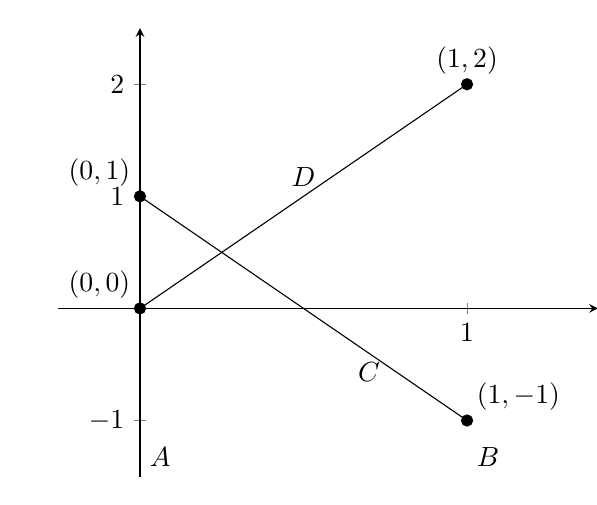
\begin{tikzpicture}
\begin{axis}[axis lines=middle, xmin=-0.25,xmax=1.4, ymin=-1.5, ymax=2.5,xtick={0,1}]
\addplot[-, mark=*]coordinates{(0,0)(1,2)}
node[pos=0,above left]{$(0,0)$}
node[pos=1,above]{$(1,2)$}
node[pos=.5,above]{$D$};

\addplot[-, mark=*]coordinates{(0,1)(1,-1)}
node[pos=0,above left]{$(0,1)$}
node[pos=1,above right]{$(1,-1)$}
node[pos=.7,below]{$C$};

\node[anchor=south west]
at ({axis cs:0,0}|-{axis description cs: 0,0}){$A$};

\node[anchor=south west]
at ({axis cs:1,0}|-{axis description cs: 0,0}){$B$};

\end{axis}
\end{tikzpicture}
\captionof{figure}{Mixed Strategy Two Lines}
   \label{F:Player 2's pure strategy D}
\end{center}   
\end{figure}

Now we can see that if Player 2 plays only D, then Player 1 does best by playing only B.
\end{itemize}

\end{itemize}

So we have this nice graph, but what does it really tell us? Although we drew lines representing each of Player 2's pure strategies, Player 1 doesn't know what Player 2 will do. Suppose Player 1 only played A, while Player 2 plays an unknown mixed strategy. Then the possible payoffs for Player 1 are 1 or 0. The more often Player 2 plays C, the more often Player 1 gets 1. So the \emph{expected payoff}\index{expected payoff} per game for a repeated game varies between 0 and 1. We can see the possible expected values as the red line on the graph in Figure \ref{F:BoldA}.

%\break

%\begin{figure}[h]
%\leavevmode
%\begin{center}
%{\scalebox{.65}{\input{graph4.pstex_t}}}
%\end{center}
%\end{figure}  
\begin{figure}
\begin{center}
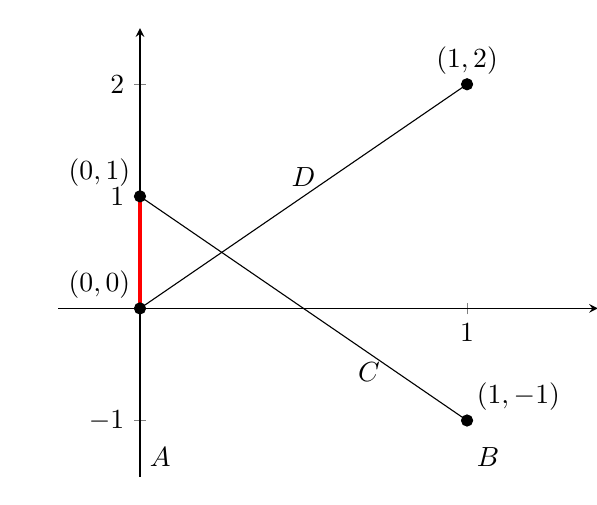
\begin{tikzpicture}
\begin{axis}[axis lines=middle, xmin=-0.25,xmax=1.4, ymin=-1.5, ymax=2.5,xtick={0,1}]
\addplot[-, mark=*]coordinates{(0,0)(1,2)}
node[pos=0,above left]{$(0,0)$}
node[pos=1,above]{$(1,2)$}
node[pos=.5,above]{$D$};

\addplot[-, mark=*]coordinates{(0,1)(1,-1)}
node[pos=0,above left]{$(0,1)$}
node[pos=1,above right]{$(1,-1)$}
node[pos=.7,below]{$C$};

\addplot[-, ultra thick, red]coordinates{(0,0)(0,1)};
%node[pos=0,above left]{$(0,1)$}
%node[pos=1,above right]{$(1,-1)$}
%node[pos=.7,below]{$C$};

\node[anchor=south west]
at ({axis cs:0,0}|-{axis description cs: 0,0}){$A$};

\node[anchor=south west]
at ({axis cs:1,0}|-{axis description cs: 0,0}){$B$};

\end{axis}
\end{tikzpicture}
\captionof{figure}{Possible expected value if Player 1 plays A}
   \label{F:BoldA}
\end{center}   
\end{figure}

Since we want to understand mixed strategies for Player 1, what would happen if Player 1 played A half the time and B half the time? In other words, what happens if $p=1/2$? Although we may not easily be able to see the exact values, we can represent the possible expected values on the graph in Figure \ref{F:BoldHalf}

%\begin{figure}[h]
%\leavevmode
%\begin{center}
%{\scalebox{.65}{\input{graph5.pstex_t}}}
%\end{center}
%\end{figure}  

\begin{figure}
\begin{center}
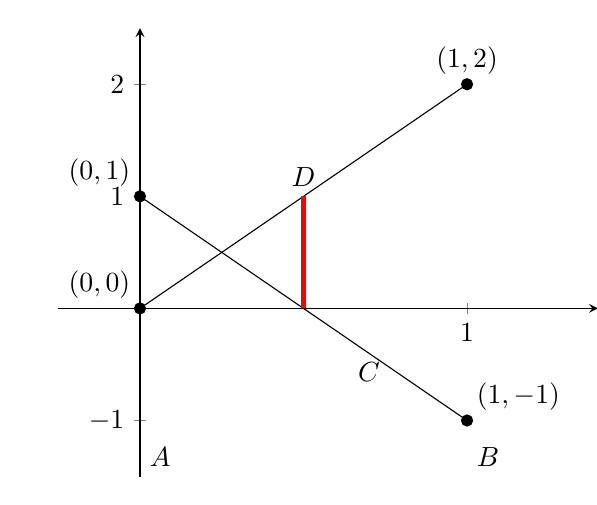
\begin{tikzpicture}
\begin{axis}[axis lines=middle, xmin=-0.25,xmax=1.4, ymin=-1.5, ymax=2.5,xtick={0,1}]
\addplot[-, mark=*]coordinates{(0,0)(1,2)}
node[pos=0,above left]{$(0,0)$}
node[pos=1,above]{$(1,2)$}
node[pos=.5,above]{$D$};

\addplot[-, mark=*]coordinates{(0,1)(1,-1)}
node[pos=0,above left]{$(0,1)$}
node[pos=1,above right]{$(1,-1)$}
node[pos=.7,below]{$C$};

\addplot[-, ultra thick, red]coordinates{(.5,0)(.5,1)};
%node[pos=0,above left]{$(0,1)$}
%node[pos=1,above right]{$(1,-1)$}
%node[pos=.7,below]{$C$};

\node[anchor=south west]
at ({axis cs:0,0}|-{axis description cs: 0,0}){$A$};

\node[anchor=south west]
at ({axis cs:1,0}|-{axis description cs: 0,0}){$B$};

\end{axis}
\end{tikzpicture}
\captionof{figure}{Player 1 plays B with probability 1/2}
   \label{F:BoldHalf}
\end{center}   
\end{figure}

Hopefully, you've begun to see that for each choice of $p$, the top line represents the highest expected value for Player 1; the bottom line represents the lowest expected value for Player 1; the area between the lines represents the possible expected values for Player 1. As we did with non-repeated games, let's look at the ``worst case scenario'' for Player 1. In other words, let's assume that Player 2 can figure out Player 1's strategy. Then Player 1 would want to \emph{maximize the minimum expected value}. Aha! This is just looking for the \emph{maximin} strategy\index{maximin strategy, repeated games}! 

Now the minimum expected value for each choice of $p$ is given by the bottom lines on the graph, shown in red in Figure \ref{F:BoldMin}.

%\begin{figure}[h]
%\leavevmode
%\begin{center}
%{\scalebox{.65}{\input{graph6.pstex_t}}}
%\end{center}
%\end{figure}  

\begin{figure}
\begin{center}
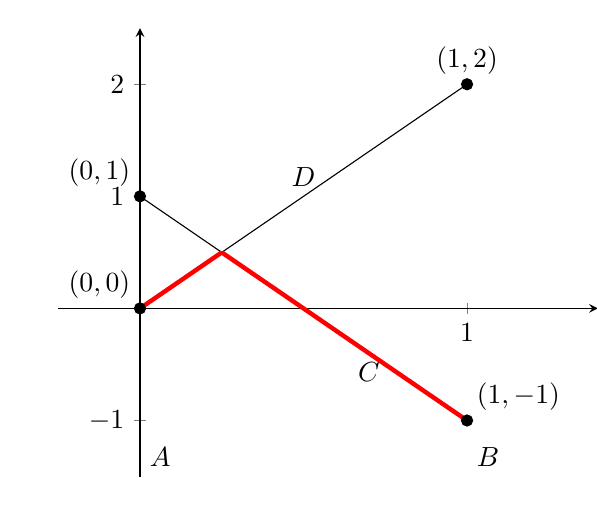
\begin{tikzpicture}
\begin{axis}[axis lines=middle, xmin=-0.25,xmax=1.4, ymin=-1.5, ymax=2.5,xtick={0,1}]
\addplot[-, mark=*]coordinates{(0,0)(1,2)}
node[pos=0,above left]{$(0,0)$}
node[pos=1,above]{$(1,2)$}
node[pos=.5,above]{$D$};

\addplot[-, mark=*]coordinates{(0,1)(1,-1)}
node[pos=0,above left]{$(0,1)$}
node[pos=1,above right]{$(1,-1)$}
node[pos=.7,below]{$C$};

\addplot[-, ultra thick, red]coordinates{(0,0)(.25,.5)};

\addplot[-, ultra thick, red]coordinates{(.25,.5)(1,-1)};
%node[pos=0,above left]{$(0,1)$}
%node[pos=1,above right]{$(1,-1)$}
%node[pos=.7,below]{$C$};

\node[anchor=south west]
at ({axis cs:0,0}|-{axis description cs: 0,0}){$A$};

\node[anchor=south west]
at ({axis cs:1,0}|-{axis description cs: 0,0}){$B$};

\end{axis}
\end{tikzpicture}
\captionof{figure}{Minimum Expected Payoff for Player 1}
   \label{F:BoldMin}
\end{center}      
\end{figure}

It should be easy to see that the \emph{maximum} of the minimum expected payoffs occurs at the intersection of the two lines.

\begin{itemize}
\item[Step 3.] Find the intersection of the two lines.
\begin{itemize}
\item[Step 3a.] Find the equation for Line C. 

This is the line passing through the points $(0, 1)$ and $(1, -1)$. It has slope $-2$ and $y$-intercept 1. Thus, it has equation $y=-2x+1$. [Although the $x$-axis represents probability $p$ and the $y$-axis represents expected payoff $m$, you are probably more comfortable solving equations--at least for the moment--in $x$ and $y$.]

\item[Step 3b.] Find the equation for Line D. 

This is the line passing through the points $(0, 0)$ and $(1, 2)$. It has slope $2$ and $y$-intercept 0. Thus, it has equation $y=2x$. 
\item[Step 3c.] Use substitution to find the point of intersection. 
\begin{eqnarray*}
2x &=&-2x+1\\
4x &=& 1\\
x&=&{1\over 4}
\end{eqnarray*}

Substituting $x={1\over 4}$ back in to either original equation, say $y=2x$, gives us $y={1\over 2}$. Thus, the point of intersection is $(1/4, 1/2)$. 
\end{itemize}

\item[Step 4.] Determine Player 1's maximin mixed strategy\index{maximin mixed strategy}. 

Recalling that the first coordinate is $p$, the probability that Player 1 plays \textbf{B}, we know that Player 1 will play B with probability 1/4, and thus, play A with probability 3/4 [$1-1/4=3/4$]. The expected payoff for Player 1 is 1/2. It is important to check back to your original intuition about the game from Exercise \ref{E:linearconjecture}. Did it seem as though Player 1 should play A more often than B?


\end{itemize}

Let's make a few important observations. First, it should be clear from the graph that Player 1 expects a payoff of 1/2 NO MATTER WHAT PLAYER 2 DOES. Furthermore, since this is a zero-sum game, we know that Player 2's expected payoff is $-1/2$. It is important to note that this graph does not give us any information about an optimal strategy for Player 2. We will see how to find a strategy for Player 2 in the following exercises. Can you think of how you might do this?


%\subsection*{Repeated Two-person Zero-Sum Games: Linear Solution}

%\markright{Repeated Games: Linear Solution}

%\vspace{.2in}

%Do all of your work on your own paper. Give complete answers (complete sentences!).


We can use the graphical method to find the maximin and minimax mixed strategies for repeated  two-person zero-sum games. 

Using the same game matrix as above: \[\left[\begin{matrix}
1&0\\
-1&2

\end{matrix}\right],
\]
we will continue to label Player 1's strategies by $A$ and $B$, and Player 2's strategies by $C$ and $D$. We now want to determine the minimax strategy for Player 2. Keep in mind the payoffs are still the payoffs to Player 1, so Player 2 wants the payoff to be as small as possible.

\begin{xca}\label{E:sketchgraphagain}
Sketch the graph for Player 1 that we drew above. Be sure to label the endpoints  of each line. Also label each line according to which strategy they represent. 
\end{xca}

\begin{xca}\label{E:showminimax}
Describe the minimax strategy\index{minimax strategy, repeated games} and show it on the graph. (You do not need to find the actual mixed strategy for Player 2.) 
\end{xca}

\begin{xca}\label{E:payoffssame}
Are the payoff vectors for the maximin and minimax strategies the same?
\end{xca}

For non-repeated games we have seen that if the maximin value is the same as the minimax value, then the game has a pure strategy equilibrium. The same idea applies to mixed strategy games. If the value of the maximin  strategy is the same as the value of the minimax strategy, then the corresponding mixed strategies will be an equilibrium point\index{mixed strategy equilibrium}\index{equilibrium, mixed strategy}. Thus, your answer to Exercise \ref{E:payoffssame} should tell you this game has a mixed strategy equilibrium point consisting of the maximin/ minimax strategy.

We now know that Player 2 wants to play the minimax strategy in response to Player 1's maximin strategy, so we need to find the actual mixed strategy for Player 2 to employ. Since we are minimizing Player 1's maximum expected payoff, we will continue to use the matrix representing Player 1's payoff. We will repeat the process we used for Player 1, except the $x$-axis now represents the probability that Player 2 will play $D$, and the lines will represent Player 1's strategies $A$ and $B$. The $y$-axis continues to represent Player 1's payoff. 

%\begin{enumerate}
%\setcounter{enumi}{3}
\begin{xca}\label{E:graphStep0}
First sketch the axes. (Recall, the $x$-axis only goes from 0 to 1.)
\end{xca}

\begin{xca}\label{E:graphP1A}
Assume Player 1 only plays $A$. 
\begin{enumerate}[(a)]
\item If Player 2 only plays $C$, what is the payoff to Player 1? Recall we called this $m$. What is the probability that Player 2 plays $D$? Recall we called this $p$. On your graph, plot the point ($p$, $m$).

\item If Player 2 plays only $D$, find $m$ and $p$. Plot $(p, m)$ on the graph.

\item Now sketch the line through your two points. This line represents Player 1's pure strategy $A$ and the expected payoff (to Player 1) for Player 2's mixed strategies. Label it $A$.
\end{enumerate}
\end{xca}

\begin{xca}\label{E:graphP1B}
Now assume Player 1 plays only $B$. Repeat the steps in Exercise \ref{E:graphP1A}, using $B$ instead of $A$, to find the line representing Player 1's pure strategy $B$. (Label it!)
\end{xca}

\begin{xca}\label{E:graphminimax} It is important to keep in  mind that although the $x$-axis refers to how often Player 2 will play $C$ and $D$, the $y$-axis represents the payoff to {\it Player 1}. 
\begin{enumerate}[(a)]
\item Explain why we are looking for the \emph{minimax} strategy for Player 2. 
\item Show on the graph the \emph{maximum} payoff that Player 1 can expect for each of Player 2's possible mixed strategies.
\item Show the point on the graph that represents the minimax strategy.
\end{enumerate}
\end{xca}

\begin{xca}\label{E:graphFindEquations}
Find the equations of the two lines.
\end{xca}

\begin{xca}\label{E:graphFindIntersection}
Find the point of intersection of the two lines.
\end{xca}

\begin{xca}\label{E:graphSolution}
How often should Player 2 play $C$? How often should he play $D$? What is Player 1's expected payoff? And hence, what is Player 2's expected payoff? 
\end{xca}


\begin{xca}\label{E:whyequil}
Explain why each player should play the maximin/ minimax mixed strategy. In other words, explain why neither player benefits by changing his or her strategy. (Hint: think about playing defensively and assuming the other player is the ``perfect'' player.)
\end{xca}


Now it may have occurred to you that since this is a zero-sum game, we could have just converted our matrix to the payoff matrix for Player 2, and found Player 2's maximin strategy. But it is important to understand the relationship between the maximin and the minimax strategies. So for the sake of practice and a little more insight \ldots

%\begin{enumerate}
%\setcounter{enumi}{11}

\begin{xca}\label{E:graphconvert}
Convert the payoff matrix above into the payoff matrix for Player 2. Find the maximin strategy for Player 2 using the graphical method. Be sure to include a sketch of the graph (labeled!!), the equations for the lines, the probability that Player 2 will play $C$ and $D$, and the expected payoff for Player 2.
\end{xca}

\begin{xca}\label{E:graphcompareapproaches}
Compare your answer in Exercise \ref{E:graphconvert} to your answer in Exercise \ref{E:graphSolution}. 
\end{xca}

\begin{xca}\label{graphfair}
Is this game fair? Explain.
\end{xca}

\begin{xca}\label{E:graphexplainEV}
We saw above that the expected payoff for Player 1 was 1/2. Explain what this means for a repeated game. (Hint: is it actually possible for a player to win 1/2 in a given game?)
\end{xca}


Now you are ready to try to analyze some more games!

%\begin{enumerate}
%\setcounter{enumi}{15}
\begin{xca}\label{E:graph2practice}
Consider the zero-sum game $\left[\begin{matrix}
-4&4\\
2&-2

\end{matrix}\right].
$
\begin{enumerate}[(a)]
\item Does this game have a pure strategy equilibrium?
\item Just by looking at the matrix, do you think this game will be fair? (Would you rather be Player 1 or Player 2?)
\item Sketch (and label!) the appropriate graph for this game.
\item Use you graph to determine if there is a mixed strategy equilibrium point. If there is, how often should Player 1 play each strategy? What is the expected payoff to each player? 
\item Is this game fair? Explain. Compare your answer to (b).
\end{enumerate}
\end{xca}

\begin{xca}\label{E:graph3practice}
Consider the zero-sum game $\left[\begin{matrix}
0&1\\
1&-10

\end{matrix}\right].
$
\begin{enumerate}[(a)]
\item Does this game have a pure strategy equilibrium?
\item Just by looking at the matrix, do you think this game will be fair? (Would you rather be Player 1 or Player 2?)

\item Sketch (and label!) the appropriate graph for this game.
\item Use you graph to determine if there is a mixed strategy equilibrium point. If there is, how often should Player 1 play each strategy? What is the expected payoff to each player? 
\item Is this game fair? Explain. Compare your answer to (b).
\end{enumerate}

\end{xca}



 

\section{Repeated Two-person Zero-Sum Games: Expected Value}\index{mixed strategies, expected value solution}\index{expected value}

%\markright{Repeated Games: Expected Value}

%\vspace{.2in}
%Do all of your work on your own paper. Give complete answers (complete sentences!).

\vspace{.1in}
In this section, we will use the idea of expected value to find the equilibrium mixed strategies for repeated two-person zero-sum games. 

One of the significant drawbacks of the graphical solution from the previous section is that it can only solve 2 X 2 matrix games. If each player has 3 options, we would need to graph in three dimensions. Technically this is possible, but rather complicated. If each player has more than 3 options, since we can't graph in four or more dimensions, we are at a complete loss. So we need to think about an alternate way to solve for the mixed strategies. Although we will begin with 2 X 2 games, this method will easily generalize to larger games.

%But now, let's think a little more about what we were really doing in the last section. The variable $x$, or $p$, represented the probability of playing a strategy. Once we knew the probability of playing strategy B, call this $P(B)$, we automatically knew the probability of playing A, $P(A)$, since the two probabilities must sum to 1. Thus, we have the equation $P(A)+P(B)=1$. 

%To find the solution in the last section, we had two equations and found their intersection point. In each equation, $y$ (or $m$) represented the expected payoff. 

\begin{example}\label{G:matching pennies}Consider the game called \emph{Matching Pennies:}\index{Matching Pennies} each player can choose HEADS (H) or TAILS (T); if the two players match, Player 1 wins; if the two players differ, Player 2 wins.
\end{example}

\begin{xca}\label{E:mpmatrix}
Determine the payoff matrix for this game. 
\end{xca}

\begin{xca}\label{E:mpnoequil}
Explain why this game has no pure strategy equilibrium point.
\end{xca}

\begin{xca}\label{E:mpguess}
Since we know that there is no pure strategy equilibrium point, we need to look for a mixed strategy equilibrium point. Just by looking at the payoff matrix, what do you think an ideal strategy for each player would be? Explain your choice. 
\end{xca}

\begin{xca}\label{E:mpguessev}
Suppose both players play your ideal strategy, what should the expected value of the game be?
\end{xca}

We could use our previous graphical method to determine the expected value of the game (you might quickly try this just to verify your prediction). However, as we have noted, a major drawback of the graphical solution is that if our players have 3 (or more) options, then we would need to graph an equation in 3 (or more!) variables; which (I hope you agree) we don't want to do.  Although we will continue to focus on $2 \times 2$ games, we will develop a new method which can more easily be used to solve to larger games. 

We will need a little notation. Let 
\begin{align}
P_1(H) & = \mbox{ the probability that Player 1 plays H; } \notag\\
P_1(T) & = \mbox{ the probability that Player 1 plays T;} \notag \\
P_2(H) & = \mbox{ the probability that Player 2 plays H; } \notag\\
P_2(T) & = \mbox{ the probability that Player 2 plays T.} \notag
\end{align}

%\begin{enumerate}
%\setcounter{enumi}{4}
\begin{xca}\label{E:mpP2 60/40}
Suppose Player 2 plays H 60\% of the time and T 40\% of the time. 
\begin{enumerate}[(a)]
\item What are $P_2(H)$ and $P_2(T)$?
\item What do you think Player 1 should do? Does this differ from your ``ideal" mixed strategy? Explain.
\item We can use expected value to compute what Player 1 should do in response to Player 2's 60/40 strategy. First, consider a pure strategy for Player 1. Compute the expected value for Player 1 if she only plays H (call it $E_1(H)$) while Player 2 plays H with probability .6  and T with probability .4.
\item Similarly, compute the expected value for Player 1 if she plays only T (call it $E_1(T)$).
\item Which pure strategy has a higher expected value for Player 1? If Player 1 plays this pure strategy, will she do better that your predicted value of the game?
\end{enumerate}
\end{xca}

\begin{xca}\label{E:mp60/40badP2}
Hopefully, you concluded that in Exercise \ref{E:mpP2 60/40} a pure strategy is good for Player 1. Explain why this means the 60/40 strategy is bad for Player 2.
\end{xca}

\begin{xca}\label{E:mpPlayH}
For any particular mixed (or pure) strategy of Player 2, we could find $E_1(T)$ and $E_1(H)$. Explain why if $E_1(H) > E_1(T)$, Player 1 should always play H. 
\end{xca}

\begin{xca}\label{E:mpPlayT}
Similarly, explain why if $E_1(H) < E_1(T)$, Player 1 should always play T. 
\end{xca}


\begin{xca}\label{E:mpuneqbad}
Explain why the situations in Exercises \ref{E:mpPlayH} and \ref{E:mpPlayT} are bad for Player 2.
\end{xca}

\begin{xca}
Use your answers from Exercises \ref{E:mpPlayH}, \ref{E:mpPlayT}, and \ref{E:mpuneqbad} to explain why the situation in which $E_1(H)=E_1(T)$ is the best for Player 2.
\end{xca}


Since we now know that Player 2 wants $E_1(H)=E_1(T)$, we can use a little algebra to compute the best defensive strategy for Player 2. Remember, we want to assume that Player 1 will always be able to chose the strategy that will be best for her, and thus Player 2 wants to protect himself. Let's find the probabilities with which Player 2 should play H  and T.

%\begin{enumerate}
%\setcounter{enumi}{10}

\begin{xca}\label{E:mpequations}
Let $P_2(H)$ and $P_2(T)$ be the probabilities that Player 2 plays H and T respectively. Find equations for $E_1(H)$ and $E_1(T)$ in terms of $P_2(H)$ and $P_2(T)$ for the game of matching pennies. Since we want $E_1(H)=E_1(T)$, set your two equations equal to each other. This gives you one equation in terms of $P_2(H)$ and $P_2(T)$.
\end{xca}

\begin{xca}\label{E:explainprobeq}
Explain why we must also have $P_2(H)+P_2(T)=1$.
\end{xca}

\begin{xca}\label{E:mpsolve}
Using the equations from Exercises \ref{E:mpequations} and \ref{E:explainprobeq}, solve for $P_2(H)$ and $P_2(T)$. You now have the equilibrium mixed strategy for Player 2. Does this match the mixed strategy you determined in Exercise \ref{E:mpguess}?
\end{xca}

\begin{xca}\label{E:mpP1sol}
Set up and solve the analogous equations from Exercises \ref{E:mpequations} and \ref{E:explainprobeq} for Player 1. (Hint: we should have an equation for $E_2(H)$ and one for $E_2(T)$. Since we are looking for the probabilities of each of Player 1's options, the equations should involve $P_1(H)$ and $P_1(T)$.) Again, does this match the mixed strategy from Exercise \ref{E:mpguess}? 
\end{xca}


We now have a new method for finding the best mixed strategies for Players 1 and 2, assuming that each player is playing defensively against an ideal player. But how can we find the value of the game?  For Player 2, we assumed $E_1(H)=E_1(T)$. In other words, we found the situation in which Player 1's expected value is the same no matter which pure strategy she plays. Thus, Player 1 is \emph{indifferent} to which pure strategy she plays. If she were not indifferent, then she would play the strategy with a higher expected value. But, as we saw, this would be bad for Player 2. So Player 1 can assume that Player 2 will play the equilibrium mixed strategy. Thus, as long as Player 1 plays a mixed strategy, it doesn't matter whether at any given time, she plays H or T (this is the idea that she is indifferent to them). Hence, the expected value of the game for Player 1 is the same as $E_1(H)$, which is the same as $E_1(T)$. Similarly, we find that the expected value of the game for Player 2 is $E_2(H)$ (or $E_2(T)$). This is a pretty complicated idea. You may need to think about it for a while.

%\begin{enumerate}
%\setcounter{enumi}{14}

 
\begin{xca}\label{E:mpEVP1}
Use the probabilities you calculated  in Exercise \ref{E:mpsolve} to find $E_1(H)$, and hence the expected value of the game for Player 1. How does this compare to your prediction for the value of the game that you gave in Exercise \ref{E:mpguessev}?
\end{xca}

\begin{xca}\label{E:mpEVP2}
Use the probabilities you calculated  in Exercise \ref{E:mpP1sol} to find $E_2(H)$, and hence the expected value of the game for Player 2. How does this compare to your prediction for the value of the game that you gave in Exercise \ref{E:mpguessev}?
\end{xca}

\begin{xca}\label{E:smallrepeatEV}
Apply this method of using expected value to Example \ref{E:smallrepeat} from the previous section to find the equilibrium mixed strategies  for each player and the value of the game for each player:
\[\left[\begin{matrix}
1&0\\
-1&2
\end{matrix}\right].
\]
\end{xca}
 
\begin{xca}\label{E:RPSEVsol}
As we noted in this section, this method can be used to solve bigger games. We just have more equations. Use the expected value method to find the equilibrium mixed strategy for Rock-Paper-Scissors\index{Rock-Paper-Scissors} for Player 2. (Hint: You will need to set $E_1(R)=E_1(P)$ and $E_1(P)=E_1(S)$; solve for $P_2(R), P_2(P), P_2(S)$; etc. It should be very similar to what you did for Matching Pennies, but there will be three equations and three unknowns.)

\end{xca}





 


\section{Repeated Two-person Zero-Sum Games: Liar's Poker}

%\markright{Liar's poker}

%\vspace{.2in}
%Do all of your work on your own paper. Give complete answers (complete sentences!).


In this section, we will continue to explore the ideas of a mixed strategy equilibrium. We have seen several examples of finding an equilibrium. We began with games which had a pure strategy equilibrium and then moved to games with mixed strategy equilibrium. We saw two different methods for finding an equilibrium. The first employed graphs in order to understand and find the maximin and minimax strategies, and hence the equilibrium mixed strategy. The second method employed the ideas of expected value to find the equilibrium strategy. We will continue to solidify these ideas with another game, a simplified variation of poker.

\begin{example}\label{liarspoker}\textbf{Liar's Poker:}\index{Liar's Poker}
We begin with a deck of cards which has 50\% aces (A) and 50\% kings (K). Aces rank higher than kings. Player 1 is dealt one card, face down. Player 1 can look at the card, but does not show the card to Player 2. Player 1 then says ``ace'' or ``king'' depending on what his card is. Player 1 can either tell the truth and say what the card is (T), or he can bluff and say that he has a higher ranking card (B). Note that if Player 1 has an ace, he must tell the truth since there are no higher ranking cards. However, if he is dealt a king, he can bluff, by saying he has an ace. If Player 1 says ``king'' the game ends and both players break even. If Player 1 says ``ace'' then Player 2 can either call (C) or fold (F). If Player 2 folds, then Player 1 wins \$0.50. If Player 2 calls and Player 1 does not have an ace, then Player 2 wins \$1. If Player 2 calls and Player 1 does have an ace, then Player 1 wins \$1.
\end{example}

\begin{xca}\label{E:PlayLP} 
Choose an opponent and play the game several times. Be sure to play the game as Player 1 and as Player 2. This is important for understanding the game. Keep track of the outcomes.
\end{xca}

\begin{xca}\label{E:LPguessstrat} 
Just from playing the game several times, can you suggest a strategy for Player 1? What about for Player 2? Does this game seem fair, or does one of the players seem to have an advantage? Explain your answers.
\end{xca}


\begin{xca}\label{E:LPguessmatrix} 
In order to formally analyze this game, we should find the payoff matrix. Do your best to find the payoff matrix. In a single hand of Liars Poker, what are the possible strategies for Player 1? What are the possible strategies for Player 2? Determine any payoffs that you can.
\end{xca}


Finding the payoff matrix in Exercise \ref{E:LPguessmatrix} is probably more challenging than it appears. Eventually we want to employ the same method for finding the payoff matrix that we used in One-Card Stud Poker from Example \ref{E:onecardstud} in Chapter 2, but first we need to understand each player's strategies, and the resulting payoffs.  We begin with the fact that Player 1 can be dealt an ace or a king. 

%\begin{enumerate}
%\setcounter{enumi}{3} 
\begin{xca}\label{E:LPP1Ace}
Assume Player 1 is dealt an ace. What can Player 1 do? What can Player 2 do? What is the payoff for each situation?
\end{xca}

\begin{xca}\label{E:LPP1King}
Assume Player 1 is dealt a king. What can Player 1 do? What can Player 2 do? What is the payoff for each situation?
\end{xca}



Since Player 1 must say ``ace'' when dealt an ace, he only has a choice of strategy when dealt a king. So we can define his strategy independent of the deal. One strategy is to say ``ace'' when dealt an ace and say ``ace'' when dealt a king; call this the \emph{bluffing strategy} (B). The other strategy is to say ``ace'' when dealt an ace and say ``king'' when dealt a king; call this the \emph{truth strategy} (T). Recall that the only time Player 2 has a choice is when Player 1 says ``ace.'' In this case Player 2 can \emph{call} (C) or \emph{fold} (F). Since we need to determine the payoff matrix, we first need to determine  the payoffs for pure strategies. This is similar to what we did for the One-Card Stud game.

%\begin{enumerate}
%\setcounter{enumi}{5}

\begin{xca}\label{E:LPBC}
Consider Player 1's pure strategy of always bluffing when dealt a king (B) and Player 2's pure strategy of always calling (C). Determine the expected value for Player 1. (Hint: you need to consider each possible deal.) What is Player 2's expected value? 
\end{xca}

\begin{xca}\label{E:LPBF}
Similarly, determine the expected value for Player 1 for the pure strategy pair \{B, F\}. What is Player 2's expected value? 
\end{xca}

\begin{xca}\label{E:LPTC}
Determine the expected value for Player 1 for the pure strategy pair \{T, C\}. What is Player 2's expected value? 
\end{xca}

\begin{xca}\label{E:LPTF}
Determine the expected value for Player 1 for the pure strategy pair \{T, F\}. What is Player 2's expected value? 
\end{xca}

\begin{xca}\label{E:LPmatrix}
Using the expected values you calculated in Exercises \ref{E:LPBC}, \ref{E:LPBF}, \ref{E:LPTC}, and \ref{E:LPTF}, set up the $2 \times 2$ payoff matrix for Liar's Poker.
\end{xca}

\begin{xca}\label{E:LPpureequil}
Using the payoff matrix you found in Exercise \ref{E:LPmatrix}, does Liar's Poker have a pure strategy equilibrium? Explain.
\end{xca}

\begin{xca}\label{E:LPmixedequil}
Use any method you have learned to find a mixed strategy equilibrium for this game. Give the mixed strategy for Player 1 and the mixed strategy for Player 2.
\end{xca}

\begin{xca}\label{E:LPcompare}
Compare your solution from Exercise \ref{E:LPmixedequil} to your conjectured strategy from Exercise \ref{E:LPguessstrat}. 
\end{xca}

\begin{xca}\label{E:LPexpectedvalue}
What is the expected value of the game for each player?  How much would Player 1 expect to win if he played 15 games using the equilibrium mixed strategy? 
\end{xca}


\begin{xca}\label{E:LPfair} 
Is this game fair? Explain. Again, compare your answer to your conjecture inExercise \ref{E:LPguessstrat}.
\end{xca}




 

\section{Augmented Matrices}\index{augmented matrix}

%\markright{Repeated Games: Expected Value}

%\vspace{.2in}
%Do all of your work on your own paper. Give complete answers (complete sentences!).


In this section, we will see how to use matrices to solve systems of equations\index{systems of equations}. In both the graphical method and the expected value method, you have had to solve a system of equations. In the graphical method you had systems consisting of two lines such as Example \ref{E:twoeq}.

\begin{example}\label{E:twoeq}
\begin{align*}
y &= \frac{3}{5}x-\frac{1}{5}\\
y &=-x+3.
\end{align*}
\end{example}

In the expected value method we had systems of three equations such as Example \ref{E:threeeq}.

\begin{example}\label{E:threeeq}
\begin{align*}
E_1(A) &= P_2(C)-P_2(D)\\
E_1(B) &= 2P_2(D)\\
1 &= P_2(C)+P_2(D).
\end{align*}
\end{example}

Even in Example \ref{E:threeeq}, the algebra began to get cumbersome. What if we wanted to solve much larger games, such as a 5 X 5 game?

In order to use matrices to solve our systems of equations, we want to write all our equations in the same form: we will have all the variable terms on the left of the equals sign and all constants on the right.

Thus, in Example \ref{E:twoeq} we can write the system as

\begin{align*}
\frac{3}{5}x-y &=\frac{1}{5}\\
x+y &= 3.
\end{align*}

In fact, we can simplify the first equation by multiplying both sides by 5:

\begin{align*}
3x-5y &=1\\
x+y &= 3.
\end{align*}

We can use the coefficients and constants to create a matrix:

\[
\left[
\begin{matrix}
3 & -5 & 1\\
1 & 1 & 3
\end{matrix}
\right].
\]

In this matrix you have a column for the coefficients of each variable. So the coefficients of $x$ are in the first column, the coefficients of $y$ are in the second. The constant terms are always in the last column. Each row corresponds to one equation.
This matrix is called an \emph{augmented matrix}\index{augmented matrix}. It is really just a matrix, but we call it \emph{augmented} if we include information from both sides of the equation (the coefficients and the constants).

The algebraic method for solving the system of equations (finding the $x$ and $y$ values that satisfy both equations) is called \emph{row reduction}. It is based on the \emph{elimination method} that you may have seen in a precalculus or college algebra course. We won't go through the algebra here, as we really don't need it. Since our goal is to be able to easily solve larger systems of equations, we will rely on technology to do the algebra. 

Computer algebra systems such as \textit{Sage}, \textit{Mathematica}, and \textit{Maple}, as well as graphing calculators, can easily do the row reduction for us. 

On your graphing calculator, use the matrix function to enter the matrix. Then use the ``rref'' function (this stands for ``reduced row echelon form'').  The result will be the following matrix:

\[
\left[
\begin{matrix}
1 & 0 & 2\\
0 & 1 & 1
\end{matrix}
\right].
\]

Recall that the first column is the $x$ and the second is the $y$. Each row represents an equation. So translating each row back to equations, we have the following system of equations:

\begin{align*}
x+0y &=2\\
0x+y &= 1
\end{align*}

or 

\begin{align*}
x &=2\\
y &= 1.
\end{align*}

By plugging these values back into the original equations, you can verify that this is in fact the solution.

Since the technology does all the algebra for us, our job is to translate the equations into an appropriate matrix and then translate the final matrix back into the solution to the system of equations. Remember, when using a matrix to solve a game, the matrix is only a tool, it is not the solution to the game.

Now, let's try the equations for the expected value method using Example \ref{E:threeeq}. As presented, how many variables does the system have?

\begin{align*}
E_1(A) &= P_2(C)-P_2(D)\\
E_1(B) &= 2P_2(D)\\
1 &= P_2(C)+P_2(D)
\end{align*}

It has 4: $E_1(A), E_1(B), P_2(C) and P_2(D)$. But when we solved these equations, we set the expected values equal. This gives us the two equations

\begin{align*}
P_2(C)-P_2(D) &= 2P_2(D)\\
1 &= P_2(C)+P_2(D).
\end{align*}

Now if we put these into the form with all variables on the left and constants on the right, we get 

\begin{align*}
P_2(C)-3P_2(D) &= 0\\
 P_2(C)+P_2(D) &= 1.
\end{align*}

Putting these equations into an augmented matrix, gives us
\[
\left[
\begin{matrix}
1 & -3 & 0\\
1 & 1 & 1
\end{matrix}
\right],
\]

where the first column corresponds to $P_2(C)$ and the second column corresponds to $P_2(D)$. Using row reduction, we get

\[
\left[
\begin{matrix}
1 & 0 & 3/4\\
0 & 1 & 1/4
\end{matrix}
\right].
\]

Thus, our solution is $P_2(C)=3/4$, and $P_2(D)=1/4$.

Here are some more systems of equations to practice solving using augmented matrices.

\begin{xca}
Solve the system of equations.

$\begin{matrix}
2x-2y&=6\\x+3y&=7
\end{matrix}$

\end{xca}


\begin{xca}
Solve the system of equations.

$\begin{matrix}
4p_1-2p_2&=0\\p_1+p_2&=1
\end{matrix}$
\end{xca}

\begin{xca} 
Consider the system of equations 

$\begin{matrix}
4x+8y-4z&=4\\3x+8y+5z&=-11\\-2x+y+12z&=-17
\end{matrix}$
\begin{enumerate}[(a)]
\item Set up the augmented matrix for this system.
%\vspace{.1in}
\item Use row reduction to find the solution.

\end{enumerate}
\end{xca}

\begin{xca}
Consider the system of equations 

$\begin{matrix}
2x+y-4z&=10\\3x+5z&=-5\\y+2z&=7
\end{matrix}$
\begin{enumerate}[(a)]
\item Set up the augmented matrix for this system.
%\vspace{.1in}
\item Use row reduction to find the solution.
 
\end{enumerate}
\end{xca}


\begin{xca}
Consider the system of equations 

$\begin{matrix}
a+b-5c&=0\\-4a-b+6c&=0\\a+b+c&=1
\end{matrix}$
\begin{enumerate}[(a)]
\item Set up the augmented matrix for this system.
%\vspace{.1in}
\item Use row reduction to find the solution.

\end{enumerate}
\end{xca}

\begin{xca}
Consider the system of equations 

$\begin{matrix}
3x+2y-w-v&=0\\2x-y+3z+w+5v&=0\\x+2y+6z-w&=0\\ -y+z-3w+v&=0\\x+y+z+w+v&=1
\end{matrix}$.
\begin{enumerate}[(a)]
\item Set up the augmented matrix for this system.
%\vspace{.1in}
\item Use row reduction to find the solution.

\end{enumerate}
\end{xca}







 
 
\section{Undercut}

%\markright{Undercut}


This section requires you to be able to solve ``large'' systems of equations. Before doing this activity you should review how to solve systems of equations using matrices and row reduction. You are encouraged to use a calculator or other technology.

%Do all of your work on your own paper. Give complete answers (complete sentences!).

As we saw in the previous section, an important part of game theory is the process of translating a game to a form that we can analyze. 

\begin{example}\label{Undercut}\textbf{Undercut:}\index{Undercut}

Each player chooses a number 1-5. If the two numbers don't differ by 1, then each player adds their own number to their score. If the two numbers differ by 1, then the player with the \emph{lower} number adds \emph{both} numbers to his or her score; the player with the higher number gets nothing.

For example, suppose in round one Player 1 chooses 4; Player 2 chooses 4. Each player keeps their own number. The score is now 4-4. In the next round, Player 1 chooses 2, Player 2 chooses 5. The score would now be 6-9. In the third round Player 1 chooses 4, Player 2 chooses 5. Now Player 1 gets both numbers, making the score 15-9.
\end{example}

\begin{xca}\label{E:Uplay}
Choose an opponent and play the game several times. Keep track of the outcomes.
\end{xca}

\begin{xca}\label{E:Uguessstrat}
Just from playing the game several times, can you suggest a strategy for Player 1? What about for Player 2? For example, what number(s) should you play most often/ least often, or does it matter? Are there numbers you should never play? Does this game seem fair, or does one of the players seem to have an advantage? Explain your answers.
\end{xca}


\begin{xca}\label{E:Upayoff}
Create a payoff matrix for this game. Note that your payoffs should have a score for each player. 
\end{xca}

\begin{xca}\label{E:Unotzerosum}
Is this a zero-sum game? Explain.
\end{xca}

\begin{xca}\label{E:Upureeq}
Does there appear to be a pure strategy equilibrium for this game? Explain.
\end{xca}

\begin{xca}\label{E:Uwinner}
How might we determine a ``winner'' for this game after playing several times? 
\end{xca}


Most likely, you said that someone will win the game if they have the most points. In fact, we probably don't care if the final score is 10-12 or 110-112. In either case, Player 2 wins. Since we will play this game several times, we do care about the point difference. For example, a score of 5-1 would be better for Player 1 than 5-3. So let's think about the game in terms of the point difference between the players in a given game. This is called the \emph{net gain}\index{net gain}. For example, with score of 5-1, Player 1 would have a net gain of 4.

%\begin{enumerate}
%\setcounter{enumi}{6} 
\begin{xca}\label{E:Unetgainex}
Calculate the net gain for Player 1 for each of the three rounds in Example \ref{Undercut} in the beginning of this section.
\end{xca}

\begin{xca}\label{E:Unetmatrix}
Create a new payoff matrix which uses the players' net gain for the payoff vectors.
\end{xca}

\begin{xca}\label{E:Uzerosum} 
Is this now a zero-sum game? Explain.
\end{xca}

\begin{xca}\label{E:Unetpureeq}
Is there a pure strategy equilibrium for this game? Explain. (Hint: rather than looking at each option, you could compare the values for the pure maximin/ minimax strategies.)
\end{xca}

\begin{xca}\label{E:Usymmetric}
This game is \emph{symmetric}\index{symmetric game}, meaning the game looks the same to Players 1 and 2. Give an example of another game which is symmetric. Give an example of a game which is \emph{not} symmetric.
\end{xca}

\begin{xca}\label{E:symmetricpayoff}
What is the expected payoff for a symmetric game? Explain your answer. (Hint: you might think about whether it is possible for a player to have an advantage in a symmetric game.)
\end{xca}


Hopefully, you determined that there is not a pure strategy equilibrium for Undercut. Thus, we would like to find a mixed strategy equilibrium. Since this is a $5 \times 5$ game, we cannot use our graphical solution. We will need to rely on our expected value solution. We want to decide with what probability we should play each number. Let $a, b, c, d, e$ be the probabilities with which Player 2 plays 1-5, respectively. For example, if Player 1 plays a pure strategy of 2, then the expected value for Player 1, $E_1(2)$, is $-3a+0b+5c-2d-3e$. 


%\begin{enumerate}
%\setcounter{enumi}{12}

\begin{xca}\label{E:Uequations}
Write down the five equations for Player 1's expected value for each of Player 1's pure strategies.
\end{xca}

\begin{xca}\label{E:Uevzero} 
In Exercise \ref{E:symmetricpayoff}, you should have determined that since this is a symmetric game, the expected value for each Player should be 0. Modify your equations to include this piece of information. It is important to recognize that this step greatly simplifies our work for the expected value method since we don't need to set the expected values equal to each other. HOWEVER, we can ONLY do this since we know the game is symmetric!
\end{xca}

\begin{xca}\label{E:Usolve}
We now have five equations and five unknowns. There is a sixth equation: we know that the probabilities must add up to 1. Use matrices to solve the resulting system of equations. Give the mixed strategy equilibrium for Player 2. What is the mixed strategy for Player 1? (Hint: should it be different than the strategy for Player 2?) 
\end{xca}



\begin{xca}\label{E:Usummary}
Based on your answer to Exercise \ref{E:Usolve}, which number(s) should you play the most often? Which should you play the least? Are there any numbers that you should never play? Compare the mathematical solution to your conjectured solution for Exercise \ref{E:Uguessstrat}. Is there an advantage to knowing the mathematical solution? 

\end{xca}




 

\chapter{Non-Zero-Sum Games}

In the previous chapters we concentrated on zero-sum games. We know how to solve any zero-sum game. If it has a pure strategy equilibrium, then we know the players should play the equilibrium strategies. If it doesn't have an equilibrium point, then we have seen methods for finding a mixed strategy equilibrium. Assuming both players are our model rational players, then we know they should always play an equilibrium strategy.

In this chapter we turn our attention to non-zero-sum games.

\section{Introduction to Two Player Non-Zero-Sum Games}\label{Intrononzero}

%\markright{Non-Zero-Sum Games}

%\vspace{.2in}
%Do all of your work on your own paper. Give complete answers (complete sentences!).


In this section we introduce non-zero-sum games. In a \emph{non-zero-sum game}\index{non-zero-sum game} the players' payoffs no longer need to sum to a constant value. Now it is possible for both players to gain or both players to lose.


\begin{xca}\label{E:propertiesnonzero}
What are some properties of a zero-sum game that may no longer hold for a non-zero-sum game? For example, in a zero-sum game is it ever advantageous to inform your opponent of your strategy? Is it advantageous to communicate prior to game play and determine a joint plan  of action? Would you still want to minimize your opponents payoff?
\end{xca}

Let's build an understanding of non-zero-sum games by looking at an example.

\begin{example}\label{E:battle of sexes}\textbf{Battle of the Sexes:}\index{Battle of the Sexes}  Alice and Bob  want to go out to a movie. Bob wants to see an action movie, Alice wants to see a comedy. Both prefer to go to a movie together rather than to go alone. We can represent the situation with the payoff matrix in Table \ref{T:battleofsexes}:

%\hspace{3in}Alice

%\begin{center}
%\begin{tabular}{l|r|c|c|}\cline{2-4}
%&&\textbf{Action}&\textbf{Comedy}\\ \cline{2-4}
%Bob&\textbf{Action} &(2, 1)&(-1, -1)\\ \cline{2-4}
%&\textbf{Comedy} &(-1, -1)&(1, 2)\\ \cline{2-4}
%\end{tabular}
%\end{center}
%\vspace{.1in}

\begin{table}[h]
\centering

\begin{tabular}{cccc}
                      & \multicolumn{3}{c}{Alice}                                                  \\ \cline{2-4} 
\multicolumn{1}{l|}{} & \multicolumn{1}{l|}{} & \multicolumn{1}{c|}{Action} & \multicolumn{1}{c|}{Comedy} \\ \cline{2-4} 
\multicolumn{1}{l|}{Bob} & \multicolumn{1}{c|}{Action} & \multicolumn{1}{c|}{$(2, 1)$} & \multicolumn{1}{c|}{$(-1, -1)$} \\ \cline{2-4} 
\multicolumn{1}{l|}{} & \multicolumn{1}{c|}{Comedy} & \multicolumn{1}{c|}{$(-1, -1)$} & \multicolumn{1}{c|}{$(1, 2)$} \\ \cline{2-4} 
\end{tabular}
\caption{Battle of the Sexes}
\label{T:battleofsexes}
\end{table}
\end{example}

%\begin{enumerate}
%\setcounter{enumi}{1}
\begin{xca}\label{E:BoSnotzerosum}
Explain why this is not a zero-sum game. 
\end{xca}

\begin{xca}\label{E:BoSannounce}
Could it be advantageous for a player to announce his or her strategy? Could it be harmful to announce his or her strategy? If possible, describe a scenario  in which it would be advantageous to announce a strategy. If possible, describe a scenario  in which it would be harmful to announce a strategy.
\end{xca}

\begin{xca}\label{E:BoSequilpoints}
Since our main goal in analyzing games has been to find equilibrium points, let's think about equilibrium points for this game. Are there any strategy pairs where players would not want to switch? [Hint: there are two!] 
\end{xca}

\begin{xca}\label{E:BoSunequal}
Are the equilibrium points the same (in other words, does each player get the same payoff at each equilibrium point)? Compare this to what must happen for zero-sum games.
\end{xca}

\begin{xca}\label{E:BoSrepeat}
Suppose the game is played repeatedly. For example, Alice and Bob have movie night once a month. Suggest a strategy for Alice and for Bob.  Feel free to play the game with someone from class. Try a playing several times \emph{without communicating} about your strategy before each game.
\end{xca}

\begin{xca}\label{E:BoScommunication}
How could communication affect the choice of strategy? Now play several times where you are allowed to communicate about your strategy. Does this change your strategy? 
\end{xca}

\begin{xca}\label{E:BoSmixedequil} 
In either case, communicating and not communicating, do you think your strategies for Alice and Bob represent a mixed strategy equilibrium?
\end{xca}

\begin{xca}\label{E:BoScomparezerosum}
In a zero-sum game, if there is a pure strategy equilibrium, then what happens when you repeat a game? If you repeat Battle of the Sexes, does the game always result in an equilibrium pair? 
\end{xca}

Hopefully, you are beginning to see some of the challenges for analyzing non-zero-sum games. We know there are equilibrium points, but even rational play may not result in an equilibrium. For the remainder of this activity, let's assume that players are \emph{not} allowed to communicate about strategy prior to play.  Such games are called \emph{non-cooperative}\index{non-cooperative games} games.

% \begin{enumerate}
%\setcounter{enumi}{9} 
\begin{xca}\label{E:BoSBobsmatrix}
Consider the game from Bob's point of view. We know that Bob wants to maximize his payoff (that has not changed). So Bob doesn't care what Alice's payoff's are. Write down Bob's payoff matrix.
\end{xca}

\begin{xca}\label{E:BoSBobgraph}
Recall that the graphical method represents Bob's expected payoff depending on how often he plays each of his options. Sketch the graph associated with Bob's payoff matrix. 
\end{xca}

\begin{xca}\label{E:BoSBobintersection}
The area between the two lines still represents the possible expected values for Bob, depending on how often Alice plays each of her strategies. So as before, the bottom lines represent the \emph{least} Bob can expect as he varies his strategy. Thus the point of intersection will represent the biggest of these smallest values (the maximin strategy). Find this point of intersection. How often should Bob play each option? What is his expected payoff?
\end{xca}


So no matter what Alice does, Bob can expect that over the long run he wins at least the value you found in Exercise \ref{E:BoSBobintersection}. Make sure you understand this before moving on.

%\begin{enumerate}
%\setcounter{enumi}{12}

\begin{xca}\label{E:BoSAlicematrix}
Now consider the game from Alice's point of view. Write down her payoff matrix and use the graphical method to find the probability with which she should play each option and her expected payoff.
\end{xca}

Now, from Exercises \ref{E:BoSBobintersection} and \ref{E:BoSAlicematrix} you have the minimum payoff each player should expect. Note that since this is not a zero-sum game, both players can expect a positive payoff. But now we want to see how this pair of mixed strategies really works for the players.

%\begin{enumerate}
%\setcounter{enumi}{13}

\begin{xca}\label{E:BoSBobsmaximin}
Assume Bob plays the mixed strategy from Exercise \ref{E:BoSBobintersection}. Calculate Alice's expected value for each of her \emph{pure} strategies ($E_2$(Comedy) and $E_2$(Action)).
\end{xca}

\begin{xca}\label{E:BoSAlicepref}
Are Alice's expected values equal? If not, which strategy does she prefer when Bob plays the mixed strategy from Exercise \ref{E:BoSBobintersection}? Does Alice want to deviate from her mixed strategy?
\end{xca}

\begin{xca}\label{E:BoSBobchange}
Now if Alice plays a pure strategy, does Bob want to change his strategy? So is the mixed strategy pair for Bob and Alice an equilibrium? In fact, if Bob changes his strategy, how does his expected value compare to the expected value for the mixed strategy?
\end{xca}

\begin{xca}\label{E:BoSgraphwrong}
What goes wrong with the graphical method in the case of a non-zero-sum game? Hint: is it important for Alice to consider the minimax strategy? Does Alice have any reason to minimize Bob's payoff?
\end{xca}

As we can see by the above example, the methods used to analyze zero-sum games may not be too helpful for non-zero-sum games. Part of the problem is that in solving zero-sum games we take into consideration that one player wants to \emph{minimize} the payoff to the other player. This is no longer the case. Changing strategies may allow BOTH players to do better. A player no longer has any reason to prevent the other player from doing better. 

%\begin{enumerate}
%\setcounter{enumi}{17}
\begin{xca}\label{E:BoSstartBmixed}
So we know the mixed strategy won't give us an equilibrium. But suppose we start there. In other words, suppose Bob plans to play the mixed strategy from Exercise \ref{E:BoSBobintersection}. Which pure strategy should Alice play? In response, which pure strategy should Bob play? What is the outcome? Do you end up at an equilibrium?
\end{xca}

\begin{xca}\label{E:BoSstartAmixed} Now suppose Alice plans to play the mixed strategy from Exercise \ref{E:BoSAlicematrix}. Calculate the expected value for Bob for each of his pure strategies. Which pure strategy does Bob prefer to play? How will Alice respond to Bob's pure strategy? What is the outcome? Do you end up at an equilibrium?
\end{xca}

\begin{xca}\label{E:BoSoutguess}
Suppose Bob thinks Alice will try the mixed strategy and Alice thinks Bob will try the mixed strategy. Which pure strategy will each play? What is the outcome? Do you end up at an equilibrium?
\end{xca}

\begin{xca}\label{E:BoSeverplaymixed}
Considering Exercises \ref{E:BoSstartBmixed}, \ref{E:BoSstartAmixed}, and \ref{E:BoSoutguess}, is it in a player's best interest to even consider playing the mixed strategy from Exercises \ref{E:BoSBobintersection} or \ref{E:BoSAlicematrix}?
\end{xca}

\begin{xca}\label{E:BoSevsol}
We have only considered the graphical method. Try applying the expected value method. What mixed strategies do you get? Explain why this method will also not result in an equilibrium. You might want to consider whether it is important for one player to minimize the expected value for the other player.
\end{xca}





 

\section{Two-Player Non-Zero-Sum Games}\label{pdandchicken}

Before getting any further into non-zero-sum games, let's recall some key ideas about zero-sum games. 
\begin{itemize}
\item If a zero-sum game has an equilibrium point, then repeating the game does not affect how the players will play. 
\item If a zero-sum game has more that one equilibrium point then the values of the equilibrium points are the same.
\item In a zero-sum game, we can find mixed strategy equilibrium points using the graphical method or the expected value method.
\item In a zero-sum game, a player never benefits from communicating her strategy to her opponent.
\end{itemize}

Hopefully, in the last section you saw that non-zero-sum games can differ on all of the above!

\begin{example}\label{E:simplenonzero}
Let's  consider the game given by Table \ref{T:simplenonzero}.
\begin{table}[h]
\centering
\begin{tabular}{rcc}
&\textbf{C}&\textbf{D}\\ 
\textbf{A} &(0, 0)&(10, 5) \\ 
\textbf{B}&(5, 10)&(0, 0) \\ 
\end{tabular}
\caption{A non-zero sum example}
\label{T:simplenonzero}
\end{table}
\end{example}

\begin{xca}\label{E:simplenzero}
Check that this is NOT a zero-sum game. 
\end{xca}

\begin{xca}\label{E:simplefindequil}
Using the ``guess and check'' method for finding equilibria, you should be able to determine that there are two equilibrium points. What are they? 
\end{xca}

\begin{xca}\label{E:simpleprefer}
As we saw in Section \ref{Intrononzero}, non-zero-sum games equilibrium points need not have the same values. Does Player 1 prefer one of these equilibria over the other?
\end{xca}

Since it is now possible for BOTH players to benefit at the same time, it might be a good idea for players to communicate with each other. For example, if Player 1 says that she will choose A no matter what, then it is in Player 2's best interest to choose D. If communication is allowed in the game, then we say the non-zero-sum game is \emph{cooperative}\index{cooperative game}. If no communication is allowed, we say it is \emph{non-cooperative}\index{non-cooperative game}. 

We saw in Section \ref{Intrononzero}, that our methods for analyzing zero-sum games do not work very well on non-zero-sum games. Let's look a little closer at this. 

If we apply the graphical method for Player 1 to the above game, we get that Player 1 should play a (1/3, 2/3) mixed strategy for an expected payoff of 10/3. Similarly we can determine that Player 2 should play a (2/3, 1/3) mixed strategy for an expected payoff of 10/3. Recall we developed this strategy as a ``super defensive'' strategy. But are our players motivated to play as defensively in a non-zero-sum game? Not necessarily! It is no longer true that Player 2 needs to keep Player 1 from gaining! 

Now suppose, Player 1 plays the (1/3, 2/3) strategy. Then the expected payoff to Player 2 for playing pure strategy C, $E_2(C)$, is 20/3; and the expected payoff to Player 2 for playing pure strategy D, $E_2(D)$, is 5/3. Thus Player 2 prefers C over D. But if Player 2 plays only C, then Player 1 should abandon her (1/3, 2/3) strategy and just play B! This results in the payoff vector (5, 10). Notice, that now the expected value for Player 1 is 5, which is better than 10/3! Again, since Player 2 is not trying to keep Player 1 from gaining, there is no reason to apply the maximin strategy to non-zero-sum games. Similarly, we don't want to apply the expected value solution since Player 1 does not care if Player 2's expected values are equal. Each player only cares about his or her own payoff, not the payoff of the other player.

OK, so now, how do we analyze these games? 

\begin{xca}\label{E:conjgeneralstrat}
What are some possible strategies for each player? Might some strategies depend on what a player knows about her opponent?
\end{xca}

Can you see that some of the analysis might be better understood with psychology than with mathematics? 





%\section{Prisoner's Dilemma and Chicken}

%\markright{Prisoner's Dilemma}

%\vspace{.2in}
%Do all of your work on your own paper. Give complete answers (complete sentences!).


In order to better understand non-zero-sum games we look at two classic games. 

%The first game is called \emph{Prisoner's Dilemma}\index{Prisoner's Dilemma}. 

\begin{example}\label{E:PrisonersDilemma}\textbf{Prisoner's Dilemma.}\index{Prisoner's Dilemma}
Two partners in crime are arrested for  burglary and sent to separate rooms. They are each offered a deal: if they confess and rat on their partner, they will receive a reduced sentence. So if one confesses and the other doesn't, the confessor only gets 3 months in prison, while the partner serves 10 years. If both confess, then they each get 8 years. However, if neither confess, there isn't enough evidence, and each gets just one year. We can represent the situation with the matrix in Table \ref{T:PrisonersDilemma}.

%\hspace{3in}Prisoner 2

%\begin{center}
%\begin{tabular}{l|r|c|c|}\cline{2-4}
%&&\textbf{Confess}&\textbf{Don't confess}\\ \cline{2-4}
%Prisoner 1&\textbf{Confess} &(8, 8)&(0.25, 10)\\ \cline{2-4}
%&\textbf{Don't confess} &(10, 0.25)&(1, 1)\\ \cline{2-4}
%\end{tabular}
%\end{center}
%\vspace{.1in}

\begin{table}[h]
\centering

\begin{tabular}{cccc}
                      & \multicolumn{3}{c}{Prisoner 2}                                                  \\ \cline{2-4} 
\multicolumn{1}{l|}{} & \multicolumn{1}{l|}{} & \multicolumn{1}{c|}{Confess} & \multicolumn{1}{c|}{Don't Confess} \\ \cline{2-4} 
\multicolumn{1}{l|}{Prisoner 1} & \multicolumn{1}{c|}{Confess} & \multicolumn{1}{c|}{$(8, 8)$} & \multicolumn{1}{c|}{$(0.25, 10)$} \\ \cline{2-4} 
\multicolumn{1}{l|}{} & \multicolumn{1}{c|}{Don't Confess} & \multicolumn{1}{c|}{$(10, 0.25)$} & \multicolumn{1}{c|}{$(1, 1)$} \\ \cline{2-4} 
\end{tabular}
\caption{Prisoner's Dilemma (years in prison)}
\label{T:PrisonersDilemma}
\end{table}
\end{example}


\begin{xca}\label{E:PDdomstrat}
Does the matrix in Table \ref{T:PrisonersDilemma} have any dominated strategies for Player 1? Does it have any dominated strategies for Player 2? Keep in mind that a prisoner prefers smaller numbers since prison time is bad.
\end{xca}

\begin{xca}\label{E:PDbeststrat}
Suppose you are Prisoner 1. What should you do? Why? Suppose you are Prisoner 2. What should you do? Why? Does your choice of strategies result in an equilibrium pair?
\end{xca}

\begin{xca}\label{E:PDbestforall}
Looking at the game as an outsider, what strategy pair is the best option for both prisoners. 
\end{xca}

\begin{xca}\label{E:PDsamedecision}
Now suppose both prisoners are perfectly rational, so that any decision Prisoner 1 makes would also be the decision Prisoner 2 makes. Further, suppose both prisoners know that their opponent is perfectly rational. What should each prisoner do?
\end{xca}

\begin{xca}\label{E:PDrandomP2}
Suppose Prisoner 2 is crazy and is likely to confess with 50/50 chance. What should Prisoner 1 do? Does it change if he confesses with a 75\% chance? What if he confesses with a 25\% chance.
\end{xca}

\begin{xca}\label{E:PDcommunicate}
Suppose the prisoners are able to communicate about their strategy. How might this affect what they choose to do?
\end{xca}

\begin{xca}\label{E:PDdilemma}
Explain why this is a ``dilemma'' for the prisoners. Is it likely they will chose a strategy which leads to the best outcome for both? You might want to consider whether there are dominated strategies.
\end{xca}

\begin{example}\label{E:Chicken}\textbf{Chicken.}\index{Chicken}
Two drivers drive towards each other. If one driver swerves, he is considered a ``chicken.'' If a driver doesn't swerve (drives straight), he is considered the winner. Of course if neither swerves, they crash and neither wins. A possible payoff matrix for this game is given in Table \ref{T:chicken}

%\hspace{3in}Driver 2

%\begin{center}
%\begin{tabular}{l|r|c|c|}\cline{2-4}
%&&\textbf{Swerve}&\textbf{Straight}\\ \cline{2-4}
%Driver 1&\textbf{Swerve} &(0, 0)&(-1, 10)\\ \cline{2-4}
%&\textbf{Straight} &(10, -1)&(-100, -100)\\ \cline{2-4}
%\end{tabular}
%\end{center}
%\vspace{.1in}

\begin{table}[h]
\centering

\begin{tabular}{cccc}
                      & \multicolumn{3}{c}{Driver 2}                                                  \\ \cline{2-4} 
\multicolumn{1}{l|}{} & \multicolumn{1}{l|}{} & \multicolumn{1}{c|}{Swerve} & \multicolumn{1}{c|}{Straight} \\ \cline{2-4} 
\multicolumn{1}{l|}{Driver 1} & \multicolumn{1}{c|}{Swerve} & \multicolumn{1}{c|}{$(0, 0)$} & \multicolumn{1}{c|}{$(-1, 10)$} \\ \cline{2-4} 
\multicolumn{1}{l|}{} & \multicolumn{1}{c|}{Straight} & \multicolumn{1}{c|}{$(10, -1)$} & \multicolumn{1}{c|}{$(-100, -100)$} \\ \cline{2-4} 
\end{tabular}
\caption{Chicken}
\label{T:chicken}
\end{table}
\end{example}


%\begin{enumerate}
%\setcounter{enumi}{7}

\begin{xca}\label{E:Cdomstrat}
Does game in Table \ref{T:chicken} have any dominated strategies?
\end{xca}

\begin{xca}\label{E:Cbestoutcome}
What strategy results in the best outcome for Driver 1? What strategy results in the best outcome for Driver 2? What happens if they both choose that strategy?
\end{xca}

\begin{xca}\label{E:Cequilpairs}
Consider the strategy pair with outcome $(-1, 10)$. Does Driver 1 have any regrets about his choice? What about Driver 2? Is this an equilibrium pair? Are there any other points in which neither driver would regret his choice?
\end{xca}

\begin{xca}\label{E:Cbeststrat}
Can you determine what each driver should do in this game? If so, does this result in an equilibrium pair?
\end{xca}

\begin{xca}\label{E:Csamestrat}
Now suppose both drivers in the game of chicken are perfectly rational, so that any decision Driver 1 makes would also be the decision Driver 2 makes. Further, suppose both drivers know that their opponent is perfectly rational. What should each driver do?
\end{xca}

\begin{xca}\label{E:Crandom} Suppose Driver 2 is a remote control dummy and will swerve or drive straight with a 50/50 chance. What should Driver 1 do? Does it change if he swerves with 75\% chance?
\end{xca}

\begin{xca}\label{E:Ccommunicate}
Can it benefit drivers in the game of chicken to communicate about their strategy? Explain.
\end{xca}

\begin{xca}\label{E:comparePDC} 
Compare Prisoner's Dilemma and Chicken. Are there dominated strategies in both games? Are there equilibrium pairs? Are players likely to reach the optimal payoff for one player, both players, or neither player? Does a player's choice depend on what he knows about his opponent (perfectly rational or perfectly random)?
\end{xca}





 
\section{A Class-Wide Experiment}\label{S:CWPD}\index{Class-Wide Prisoner's Dilemma}

We are going to look at a class-wide game. 

%I am sending this email to the [20] of you in Introduction to Game Theory. I am proposing to all of you a game, the payoffs will be in real homework points. Any points you earn will be extra-credit points and added to your current homework points.  The game is simple. Here is how it goes.

Each member of the class secretly chooses a single letter: ``C'' or ``D,'' standing for ``cooperate''\index{cooperate} or ``defect.''\index{defect} This will be used as your strategy choice in the following game with each of the other players in the class. Here is how it works for each pair of players:  if they both cooperate, they get each get 3 points. If they both defect, they each get 1 point. If one cooperates and one defects, the cooperator gets nothing, but the defector gets 5 points. Your one choice of ``C'' or ``D'' will be used to play the game with all the other players in the class. 

Thus, if everyone chooses ``C,'' everyone will get 3 points per person (not counting yourself). If everyone chooses ``D,'' everyone will get  1 point per person (not counting yourself). You can't lose! And of course, anyone chooses ``D'' will get at least as much as everyone else will. If, for example in a class of 20, 11 people send in ``C'' and 9 send in ``D,'' then the 11 C-ers will get 3 points apiece from the other C-ers (making 30 points), and zero from the D-ers. So C-ers will get 30 points each. The D-ers, by contrast, will pick up 5 points apiece from each of the C-ers, making 55 points, and 1 point from each of the other D-ers, making 8 points, for a grand total of 63 points. No matter what the distribution is, D-ers always do better than C-ers. Of course, the more C-ers there are, the better everyone will do!

By the way, I should make it clear that in making your choice, you should not aim to be the winner, but simply to get as many points for yourself as possible. Thus you should be happier to get 30 points (as a result of saying ``C'' along with 10 others, even though the 9 D-sayers get more than you) than to get 19 points (by saying ``D'' along with everybody else, so nobody ``beats'' you). 

Of course, your hope is to be the only defector, thus really cleaning up: with 19 C-ers, you'll get 95 points, and they'll each get 18 times 3, namely 54 points! But why am I doing the multiplication or any of this figuring for you? You've been studying game theory. So have all of you! You are all equally versed in game theory and understand about making rational choices. Therefore, I hardly need to tell you that you are to make what you consider to be your maximally rational choice. In particular, feelings of morality, guilt, apathy, and so on, are to be disregarded. Reasoning alone (of course including reasoning about others' reasoning) should be the basis of your decision.

So all you need to do is make your choice. Write it down.

It is to be understood (it almost goes without saying, but not quite) that you are not to discuss your answer with anyone else from the class. The purpose is to see what people do on their own, in isolation. Along with your answer you should include a short explanation for why you made your particular choice.

%In summary, send me your choice ``C" or ``D" and a brief explanation of your choice no later than [12 noon Monday]. Late responses will not be counted. 

%ALSO, DO NOT REPY TO THE ENTIRE LIST. Respond only to me [email address].

%{\bf Any response to the entire list will disqualify you from the game.}
%\bigskip

%Good Luck!

[Adapted from Douglas Hofstadter, \textit{Metamagical Themas}]

------------------------------------------

\break

\begin{xca}\label{E:CWPDsummary}
Once everyone in class has made his or her choice, share your answers with the class.
\begin{enumerate}[(a)]
\item How many C's were there?
\item How many D's were there?
\item What was the payoff to each C?
\item What was the payoff to each D?
\end{enumerate}
\end{xca}

\begin{xca}\label{E:CWPDmatrix}
Determine the payoff matrix for class-wide Prisoner's Dilemma. [Hint: although you played this game with each other person in the class, this is still a 2 person game!]
\end{xca}

\begin{xca}\label{E:CWPDreasons}
What are some reasons people chose C? What are some reasons people chose D? 
\end{xca}

\begin{xca}\label{E:CWPDrational} 
Let's think about the idea of \emph{rationality}. What appears to be the most rational choice, C or D? If everyone is \emph{equally} rational, then what would everyone do? If everyone is equally rational, should everyone choose the same thing?
\end{xca}

\begin{xca}\label{E:CWPDsame}
Now suppose everyone is equally (and perfectly) rational. AND everyone knows that everyone else is equally (and perfectly) rational. What should everyone choose? [Hint: if everyone knows that everyone will choose the same answer, what should everyone choose to do?]
\end{xca}

\begin{xca}\label{E:PDvariant1}
Consider the game in Table \ref{T:PDvariant1} 

\begin{table}[h]
\begin{tabular}{rcc}
&\textbf{C}&\textbf{D}\\ 
\textbf{C} &(3, 3)&(0, 50) \\ 
\textbf{D}&(50, 0)&(.01, .01) \\ 
\end{tabular}
\caption{Matrix for Exercise \ref{E:PDvariant1}}
\label{T:PDvariant1}
\end{table}

What would you do? Why? What seems to be the most rational thing to do? Why?
\end{xca}

\begin{xca}\label{E:PDvariant2}
Consider the game in Table \ref{T:PDvariant2}
 
\begin{table}[h]
\begin{tabular}{rcc}
&\textbf{C}&\textbf{D}\\ 
\textbf{C} &(1000, 1000)&(0, 100) \\ 
\textbf{D}&(100, 0)&(100, 100) \\ 
\end{tabular}
\caption{Matrix for Exercise \ref{E:PDvariant2}}
\label{T:PDvariant2}
\end{table}

What would you do? Why? What seems to be the most rational thing to do? Why?
\end{xca}

\begin{xca}\label{E:CWPDpayoffs} 
Looking at all three of the above games, can you think of what sort of payoffs you would need in order to cooperate (C)? What about to defect (D)?
\end{xca}


\section{What Makes a Prisoner's Dilemma?}\label{S:PDconditions}

%\markright{Class-wide Prisoner's Dilemma}

%\vspace{.2in}
%Do all of your work on your own paper. Give complete answers (complete sentences!).

In this section we give mathematical description of Prisoner's Dilemma and compare it to some similar games.

The Class-wide Prisoner's Dilemma game we played has the payoff matrix  given in Table \ref{T:CWPD}for each pair of players.
 
%\hspace{3in}Player 2

%\begin{center}
%\begin{tabular}{l|r|c|c|}\cline{2-4}
%&&\textbf{Cooperate}&\textbf{Defect}\\ \cline{2-4}
%Player 1&\textbf{Cooperate} &(3, 3)&(0, 5)\\ \cline{2-4}
%&\textbf{Defect} &(5, 0)&(1, 1)\\ \cline{2-4}
%\end{tabular}
%\end{center}
%\vspace{.1in}

\begin{table}[h]
\centering

\begin{tabular}{cccc}
                      & \multicolumn{3}{c}{Player 2}                                                  \\ \cline{2-4} 
\multicolumn{1}{l|}{} & \multicolumn{1}{l|}{} & \multicolumn{1}{c|}{Cooperate} & \multicolumn{1}{c|}{Defect} \\ \cline{2-4} 
\multicolumn{1}{l|}{Player 1} & \multicolumn{1}{c|}{Cooperate} & \multicolumn{1}{c|}{$(3, 3)$} & \multicolumn{1}{c|}{$(0, 5)$} \\ \cline{2-4} 
\multicolumn{1}{l|}{} & \multicolumn{1}{c|}{Defect} & \multicolumn{1}{c|}{$(5, 0)$} & \multicolumn{1}{c|}{$(1, 1)$} \\ \cline{2-4} 
\end{tabular}
\caption{Class-wide Prisoner's Dilemma}
\label{T:CWPD}
\end{table}

We can classify each of the values for the payoffs as follows:
\begin{itemize}
\item  Reward for Mutual Cooperation: $R=3.$
\item Punishment for Defecting: $P=1.$
\item Temptation to Defect: $T=5.$
\item Sucker's Payoff: $S=0.$
\end{itemize}

In order for a game to be a variation of Prisoner's Dilemma it must satisfy two conditions:
\begin{enumerate}[(A)]
\item $T>R>P>S$
\item $(T+S)/2 < R$
\end{enumerate}

Let's apply this description of Prisoner's Dilemma to a few games we've seen.


\begin{xca}\label{E:describeconditions}
Describe each of the conditions (A) and (B) in words. Hint: $(T+S)/2$ is the average of $T$ and $S$.
\end{xca}
%\item Why do you think each of these conditions is required for a Prisoner's Dilemma? You might think about what would happen if each of the conditions were false. For example, what would change if $T<R$? Would players be likely to play differently? 

\begin{xca}\label{E:CWPDshow}
Show that the two conditions hold for the Class-wide Prisoner's Dilemma.
\end{xca}

\begin{xca}\label{E:PDshow}
Recall the matrix for Prisoner's Dilemma from Example \ref{E:PrisonersDilemma}.

%\hspace{3in}Prisoner 2

%\begin{center}
%\begin{tabular}{l|r|c|c|}\cline{2-4}
%&&\textbf{Confess}&\textbf{Don't confess}\\ \cline{2-4}
%Prisoner 1&\textbf{Confess} &(8, 8)&(0.25, 10)\\ \cline{2-4}
%&\textbf{Don't confess} &(10, 0.25)&(1, 1)\\ \cline{2-4}
%\end{tabular}
%\end{center}
%\vspace{.1in}
\begin{table}[h]
\centering

\begin{tabular}{cccc}
                      & \multicolumn{3}{c}{Prisoner 2}                                                  \\ \cline{2-4} 
\multicolumn{1}{l|}{} & \multicolumn{1}{l|}{} & \multicolumn{1}{c|}{Confess} & \multicolumn{1}{c|}{Don't Confess} \\ \cline{2-4} 
\multicolumn{1}{l|}{Prisoner 1} & \multicolumn{1}{c|}{Confess} & \multicolumn{1}{c|}{$(8, 8)$} & \multicolumn{1}{c|}{$(0.25, 10)$} \\ \cline{2-4} 
\multicolumn{1}{l|}{} & \multicolumn{1}{c|}{Don't Confess} & \multicolumn{1}{c|}{$(10, 0.25)$} & \multicolumn{1}{c|}{$(1, 1)$} \\ \cline{2-4} 
\end{tabular}
\caption{Prisoner's Dilemma (again)}
%\label{T:PrisonersDilemma2}
\end{table}



Determine $R, P, T,$ and $S$ for this game. Be careful: think about what cooperating versus defecting should mean. Show the conditions for Prisoner's Dilemma are satisfied. (Hint: time in jail is bad, so the bigger the number, the worse you do; thus, it might be helpful to think of the payoffs as negatives.)
\end{xca}

\begin{xca}\label{E:chickenshow}
Recall the matrix for Chicken from Example \ref{E:Chicken}.

%\hspace{3in}Driver 2

%\begin{center}
%\begin{tabular}{l|r|c|c|}\cline{2-4}
%&&\textbf{Swerve}&\textbf{Straight}\\ \cline{2-4}
%Driver 1&\textbf{Swerve} &(0, 0)&(-1, 10)\\ \cline{2-4}
%&\textbf{Straight} &(10, -1)&(-100, -100)\\ \cline{2-4}
%\end{tabular}
%\end{center}
%\vspace{.1in}
\begin{table}[h]
\centering

\begin{tabular}{cccc}
                      & \multicolumn{3}{c}{Driver 2}                                                  \\ \cline{2-4} 
\multicolumn{1}{l|}{} & \multicolumn{1}{l|}{} & \multicolumn{1}{c|}{Swerve} & \multicolumn{1}{c|}{Straight} \\ \cline{2-4} 
\multicolumn{1}{l|}{Driver 1} & \multicolumn{1}{c|}{Swerve} & \multicolumn{1}{c|}{$(0, 0)$} & \multicolumn{1}{c|}{$(-1, 10)$} \\ \cline{2-4} 
\multicolumn{1}{l|}{} & \multicolumn{1}{c|}{Straight} & \multicolumn{1}{c|}{$(10, -1)$} & \multicolumn{1}{c|}{$(-100, -100)$} \\ \cline{2-4} 
\end{tabular}
\caption{Chicken (again)}
%\label{T:chicken}
\end{table}

Determine $R, P, T,$ and $S$ for this game. Again, think about what cooperating and defecting mean in this game. Determine if the conditions for Prisoner's Dilemma are satisfied. If not, which condition(s) fail?
\end{xca}

\begin{xca}\label{E:conditionspractice1} 
Consider the game:
\[\begin{matrix}
& C& D\\
C& (3, 3) & (0, 50)\\
D &(50, 0) & (.01, .01)
\end{matrix}\]

Determine $R, P, T,$ and $S$ for this game. Determine if the conditions for Prisoner's Dilemma are satisfied. If not, which condition(s) fail?
\end{xca}

\begin{xca}\label{E:conditionspractice2}
Consider the game:
\[\begin{matrix}
& C& D\\
C& (1000, 1000) & (0, 100)\\
D &(100, 0) & (100, 100)
\end{matrix}\]
Determine $R, P, T,$ and $S$ for this game. Determine if the conditions for Prisoner's Dilemma are satisfied. If not, which condition(s) fail?
\end{xca}

\begin{xca}\label{E:conditionscompare}
The games in Exercises \ref{E:chickenshow}, \ref{E:conditionspractice1}, and \ref{E:conditionspractice2} are not true Prisoner's Dilemmas. For each game, how do the changes in payoffs affect how you play? In particular, in Prisoner's Dilemma, a player will generally choose to defect. This results in a non-optimal payoff for each player. Is this still true in Exercises \ref{E:chickenshow}, \ref{E:conditionspractice1}, and \ref{E:conditionspractice2}? If possible, use the changes in the conditions (A) and (B) to help explain any differences in how one should play. 
\end{xca}


We can define \emph{defection}\index{defection} as the idea that if everyone did it, things would be worse for everyone. Yet, if only one (or a small) number did it, life would be sweeter for that individual. We can define \emph{cooperation}\index{cooperation} as the act of resisting temptation for the betterment of all players.

%\begin{enumerate}
%\setcounter{enumi}{7}

\begin{xca}\label{E:reallifeex}
Give an example of defection and cooperation from real life.
\end{xca}

%\item Read the ``Tale of Happiton" [{\it Metamagical Themas}, D. Hofstadter, p.767] Write a short essay relating the story to a current political, environmental, or social issue.





 
 
\section{Another Multiplayer Experiment}\label{VDexperiment}

This activity needs to be played as a class. All players need to be able to respond without being able to see the responses of others. Answers may be revealed before moving on to the next question.

Without sharing your answers with others, select your answer to the following questions. Try to be as honest about your answer as possible.  Make sure you have a reason for each answer.

\begin{enumerate}
\item The lights go out in the neighborhood. Someone needs to call the power company. If someone calls, everyone's lights go on.

\begin{enumerate}
\item Call
\item Don't call
\end{enumerate}

\item The same as in (1), but now you have to wait on hold for 5 minutes.

\begin{enumerate}
\item Call
\item Don't call
\end{enumerate}

\item The same as in (1), but now you have to wait on hold for 30 minutes.

\begin{enumerate}
\item Call
\item Don't call
\end{enumerate}

\item The same as in (1), but now you have to pay a \$.50 service fee.

\begin{enumerate}
\item Call
\item Don't call
\end{enumerate}

\item The same as in (1), but now you have to pay a \$2.50 service fee.

\begin{enumerate}
\item Call
\item Don't call
\end{enumerate}

\item The phone lines go down in your small mountain community. You have to hike 3 miles in the snow to notify the power company.

\begin{enumerate}
\item Hike to notify the phone company
\item Stay home and let someone else do the hiking
\end{enumerate}

\item Everyone in your class cheats on an exam. The professor says if someone confesses they receive an F. If no one confesses, everyone fails.

\begin{enumerate}
\item Confess
\item Don't confess
\end{enumerate}

\item Evil Dr. No captures the class and puts you in all in a shark tank separated so you can't communicate. If one person volunteers to be eaten then the rest go free. If no one volunteers after 10 minutes all get eaten by sharks.

\begin{enumerate}
\item Volunteer
\item Don't volunteer
\end{enumerate}

\item Evil Dr. No captures your family and puts you in all in a shark tank separated so you can't communicate. If one person volunteers to be eaten then the rest go free. If no one volunteers after 10 minutes all get eaten by sharks.

\begin{enumerate}
\item Volunteer
\item Don't volunteer
\end{enumerate}

\item For any ``Big Brother'' fans. Choose to eat all your favorite foods for a week or nasty ``slop'' for a week. If at least three people say slop, everyone gets what they asked for. Otherwise everyone is on slop.

\begin{enumerate}
\item Favorite foods
\item Slop
\end{enumerate}

\item OK, now let's get serious about this. Answer 5 points or 1 point. If at least one person says 1 point, everyone gets the number of points they chose. Otherwise, everyone gets 0 points.

\begin{enumerate}
\item 5 points
\item 1 point
\end{enumerate}

\item Answer 20 points or 1 point. If at least one person says 1 point, everyone gets the number of points they chose. Otherwise, everyone gets 0 points.

\begin{enumerate}
\item 20 points
\item 1 point
\end{enumerate}

\item Answer 6 points or 5 points. If at least one person says 5 points, everyone gets the number of points they chose. Otherwise, everyone gets 0 points.

\begin{enumerate}
\item 6 points
\item 5 points
\end{enumerate}

\item Answer 20 points or 1 point. If at least \emph{five}  people say 1 point, everyone gets the number of points they chose. Otherwise, everyone gets 0 points.

\begin{enumerate}
\item 20 points
\item 1 point
\end{enumerate}
\end{enumerate}
-----------------------------------------------------


\begin{xca} After answering the questions, were you likely to volunteer or unlikely to volunteer? For example, were you likely to be the one to call the power company or get eaten by sharks, or were you generally hoping someone else would do it? If it depended on the situation, explain under what circumstances you were likely to volunteer.
\end{xca}

\begin{xca}
After sharing your answers as a class, did each situation have a volunteer? In other words, was there always someone willing to call the power company or take fewer points? If there was a question with no volunteer, can you suggest why?
\end{xca} 

\begin{xca}
For which questions was it unlikely that there would be very many volunteers? Did you take that into consideration when deciding if you were going to volunteer?
\end{xca}

\begin{xca}
What are some reasons for volunteering? What are some reasons not to volunteer?
\end{xca}


\section{Volunteer's Dilemma}

%\markright{Volunteer's Dilemma}

%\vspace{.2in}
%Do all of your work on your own paper. Give complete answers (complete sentences!).

\vspace{.1in}
In Section \ref{VDexperiment} we played a game called Volunteer's Dilemma\index{Volunteer's Dilemma}. 
\begin{example}\label{E:VDpoints}
One example of a Volunteer's Dilemma is the game where everyone chooses ``1 point'' or ``5 points.'' If at least one person writes down 1 point, then everyone gets the number of points they wrote down. If no one chooses 1 point, then everyone gets 0 points. Choosing ``1 point'' is considered volunteering or cooperating. Choosing to not volunteer and take ``5 points'' is defecting.

You should note that it is difficult to put this game into a matrix form since payoffs depend on whether there is at least one volunteer or cooperator. 
\end{example}

In this section we will compare Class-wide Prisoner's Dilemma with Volunteer's Dilemma. We will use the payoffs for Prisoner's Dilemma from Section \ref{S:CWPD}, given again in Table \ref{T:CWPD2}.

%\hspace{3in}Player 2

%\begin{center}
%\begin{tabular}{l|r|c|c|}\cline{2-4}
%&&\textbf{Cooperate}&\textbf{Defect}\\ \cline{2-4}
%Player 1&\textbf{Cooperate} &(3, 3)&(0, 5)\\ \cline{2-4}
%&\textbf{Defect} &(5, 0)&(1, 1)\\ \cline{2-4}
%\end{tabular}
%\end{center}
%\vspace{.1in}

\begin{table}[h]
\centering

\begin{tabular}{cccc}
                      & \multicolumn{3}{c}{Player 2}                                                  \\ \cline{2-4} 
\multicolumn{1}{l|}{} & \multicolumn{1}{l|}{} & \multicolumn{1}{c|}{Cooperate} & \multicolumn{1}{c|}{Defect} \\ \cline{2-4} 
\multicolumn{1}{l|}{Player 1} & \multicolumn{1}{c|}{Cooperate} & \multicolumn{1}{c|}{$(3, 3)$} & \multicolumn{1}{c|}{$(0, 5)$} \\ \cline{2-4} 
\multicolumn{1}{l|}{} & \multicolumn{1}{c|}{Defect} & \multicolumn{1}{c|}{$(5, 0)$} & \multicolumn{1}{c|}{$(1, 1)$} \\ \cline{2-4} 
\end{tabular}
\caption{Class-wide Prisoner's Dilemma (again)}
\label{T:CWPD2}
\end{table}


 
\begin{xca}\label{E:CWPDdefecteffect}
In Class-wide \textbf{Prisoner's Dilemma} what effect does one defector have on the group? In other words, if a single player defects, how many points does he cost each of the other players?
\end{xca}

\begin{xca}\label{E:CWPDalldefecteffect}
In Class-wide \textbf{Prisoner's Dilemma} what effect does everyone's defection have on the group? In other words, what is the most points lost by the group if everyone defects?
\end{xca}

\begin{xca}\label{E:CWPDowndefect} 
In class-wide \textbf{Prisoner's Dilemma} what effect could your own defection have on the group? In other words, how many points does the group lose if you defect instead of cooperate? You may need to consider different cases depending on how many cooperators there are. For example what if there are no cooperators? What if there are no defectors? What if there are some of each?
\end{xca}

\begin{xca}\label{E:VDdefecteffect} 
In \textbf{Volunteer's Dilemma}, with the payoffs given in Example \ref{E:VDpoints}, what effect does one defector have on the group? In other words, if there is a single defector, how many points do each of the other players lose?
\end{xca}

\begin{xca}\label{E:VDalldefecteffect} 
In \textbf{Volunteer's Dilemma}, with the payoffs given in Example \ref{E:VDpoints}, what effect does everyone's defection have on the group? In other words, if everyone defects, how many points does the group lose?
\end{xca}

\begin{xca}\label{E:VDowndefect} 
In {\bf Volunteer's Dilemma}, with the payoffs given in Example \ref{E:VDpoints}, what effect could your own defection have on the group? In other words, how many points does the group lose if you defect instead of cooperate? You may need to consider different cases depending on how many cooperators there are. For example what if there are no cooperators? What if there are no defectors? What if there are some of each?
\end{xca}

\begin{xca}\label{E:CWPDcoopordefect} 
Considering your answers above and to previous work with Prisoner's Dilemma, in Class-wide \textbf{Prisoner's Dilemma}, which is more \emph{rational} to be a cooperator or a defector? Why?
\end{xca} 

\begin{xca}\label{E:CWPDallrational}
Whichever you chose in Exercise \ref{E:CWPDcoopordefect}, explain what would happen if everyone was the most rational. Is it now more rational to do the opposite?
\end{xca}

\begin{xca}\label{E:VDcoopordefect}
Considering your answers above, in \textbf{Volunteer's Dilemma}, which is more \emph{rational} to be a cooperator (volunteer) or a defector? Why?
\end{xca}


\begin{xca}\label{E:VDallrational}
Whichever you chose in Exercise \ref{E:VDcoopordefect}, explain what would happen if everyone was the most rational. Is it now more rational to do the opposite?
\end{xca}

\begin{xca}\label{E:classchicken}  
Volunteer's Dilemma can also be called ``Class-wide Chicken.'' Try to describe this class-wide game in terms of ``swerving'' and ``going straight.'' How do the payoffs for Volunteer's Dilemma relate to the payoffs for Chicken?
\end{xca}





 

\section{Repeated Prisoner's Dilemma}

%\markright{Repeated Prisoner's Dilemma}

%\vspace{.2in}
%Do all of your work on your own paper. Give complete answers (complete sentences!).


In this section we look at two players playing Prisoner's Dilemma repeatedly. We call this game an \emph{iterated} Prisoner's Dilemma\index{iterated Prisoner's Dilemma}.
Recall the general Prisoner's Dilemma matrix from previous sections, given again in Table \ref{T:CWPD3}.

%\hspace{3in}Player 2

%\begin{center}
%\begin{tabular}{l|r|c|c|}\cline{2-4}
%&&\textbf{Cooperate}&\textbf{Defect}\\ \cline{2-4}
%Player 1&\textbf{Cooperate} &(3, 3)&(0, 5)\\ \cline{2-4}
%&\textbf{Defect} &(5, 0)&(1, 1)\\ \cline{2-4}
%\end{tabular}
%\end{center}
%\vspace{.1in}

\begin{table}[h]
\centering

\begin{tabular}{cccc}
                      & \multicolumn{3}{c}{Player 2}                                                  \\ \cline{2-4} 
\multicolumn{1}{l|}{} & \multicolumn{1}{l|}{} & \multicolumn{1}{c|}{Cooperate} & \multicolumn{1}{c|}{Defect} \\ \cline{2-4} 
\multicolumn{1}{l|}{Player 1} & \multicolumn{1}{c|}{Cooperate} & \multicolumn{1}{c|}{$(3, 3)$} & \multicolumn{1}{c|}{$(0, 5)$} \\ \cline{2-4} 
\multicolumn{1}{l|}{} & \multicolumn{1}{c|}{Defect} & \multicolumn{1}{c|}{$(5, 0)$} & \multicolumn{1}{c|}{$(1, 1)$} \\ \cline{2-4} 
\end{tabular}
\caption{A Prisoner's Dilemma matrix}
\label{T:CWPD3}
\end{table}


\begin{xca}\label{E:internetpurchaseonce}
Suppose this represented the situation of purchasing an item (say, a collectable Star Wars action figure) on the internet where both parties are untraceable. You agree to send the money at the same time that the seller agrees to send the toy. Then we can think of Cooperating as each of you sending money/ toy, and Defecting as not sending money/ toy. What should you do and why?
\end{xca}

\begin{xca}\label{E:internetpurchaserepeat}
Now suppose you wish to continue to do business with the other party. For example, instead of buying a Star Wars action figure, maybe you are buying music downloads. What should you do and why?
\end{xca}

\begin{xca}\label{E:RPDstrategy}
Suggest a strategy for playing the Prisoner's Dilemma in Table \ref{T:CWPD3} repeatedly. DON'T SHARE YOUR STRATEGY WITH ANYONE YET! 
\end{xca}

\begin{xca}\label{E:RPDplay}
Play 10 rounds of Prisoner's Dilemma with someone in class. Use your suggested strategy. Keep track of the payoffs. Did your strategy seem effective? What should it mean to have an ``effective'' strategy?
\end{xca}

We are now going to play a Prisoner's Dilemma Tournament! Choose one of the strategies below. You are to play your strategy against everyone else in the class. Keep a running total of your score. Don't tell your opponents your strategy. 


Some possible strategies:

\begin{itemize}
\item Strategy: {\bf Defection.} Your strategy is to {\it always} choose DEFECT (D).
\vspace{.2in}
\item Strategy: {\bf Cooperation.} Your strategy is to {\it always} choose COOPERATE (C).
\vspace{.2in}
\item Strategy: {\bf Tit for Tat.} Your strategy is to play whatever your opponent just played. Your first move is to COOPERATE (C), but then you need to repeat your opponent's last move. 
\vspace{.2in}

\item Strategy: {\bf Tit for Two Tats.} Your strategy is to COOPERATE (C) unless your opponent DEFECTS twice in a row. After two D's you respond with D. 
\vspace{.2in}

\item Strategy: {\bf Random (1/2, 1/2).} Your strategy is to COOPERATE (C) randomly 50\% of the time and DEFECT (D) 50\% of the time. [Note: it will be hard to be truly random, but try to play each option approximately the same amount.]
\vspace{.2in}

\item Strategy: {\bf Random (3/4, 1/4).} Your strategy is to COOPERATE (C) randomly 75\% of the time and DEFECT (D) 25\% of the time. [Note: it will be hard to be truly random, but try to play C more often than D.]
\vspace{.2in}

\item Strategy: {\bf Random (1/4, 3/4).} Your strategy is to COOPERATE (C) randomly 25\% of the time and DEFECT (D) 75\% of the time. [Note: it will be hard to be truly random, but try to play D more often than C.]
\vspace{.2in}

\item Strategy: {\bf Tit for Tat with Occasional Surprise D.} Your strategy is to play whatever your opponent just played. Your first move is to COOPERATE (C), but then you need to repeat your opponent's last move. Occasionally, you will deviate from this strategy by playing D.
\vspace{.2in}
\end{itemize}


%\begin{enumerate}
%\setcounter{enumi}{4}
\begin{xca}\label{E:RPDplaytournament}
WITHOUT SHARING YOUR STRATEGY, play Prisoner's Dilemma 10 times with each of the other members of the class. Keep track of the payoffs for each game and your total score.
\end{xca}

\begin{xca}\label{E:RPDeffectivestrategies}
After playing Repeated Prisoner's Dilemma as a class, can you determine who had which strategy? At this point you may share your strategy with others. Was your strategy more effective with some strategies than with others? Describe which opponents' strategies seemed to give you more points, which seemed to give you fewer?
\end{xca}

\begin{xca}\label{E:RPDbeststrategies}
Describe the strategy or strategies that had the highest scores in the tournament. Does this seem surprising? Why or why not? How do the winning strategies compare to the strategy you suggested in Exercise \ref{E:RPDstrategy}?
\end{xca}

\begin{xca}\label{E:RPDcompare}
How does Repeated Prisoner's Dilemma differ from the ``one-time'' Prisoner's Dilemma? Try to think in terms of rational strategies.
\end{xca}

\begin{xca}\label{E:RPDreallife}
Describe a situation from real life that resembles a Repeated Prisoner's Dilemma. 
\end{xca}

Repeated or Iterated Prisoner's Dilemma has applications to biology and sociology. If you think of higher point totals as ``success as a species'' in biology or ``success of a society'' in sociology, we can try to determine which strategies seem the most effective or successful.

%\begin{enumerate}
%\setcounter{enumi}{9}

\begin{xca}\label{E:RPDfewdefect}
How do a few defectors fare in a society of mostly cooperators? How do the cooperators fare?  (In other words, who will be more successful?) Keep in mind that everyone is playing with lots of cooperators and only a few defectors. Who will have the most points, cooperators or defectors?
\end{xca}

\begin{xca}\label{E:RPDfewcoop} 
How do a few cooperators fare in a society of mostly defectors? How do the defectors fare? (In other words, who will be more successful?) Keep in mind that everyone is playing with lots of defectors and only a few cooperators. Who will have the most points, cooperators or defectors?
\end{xca}

\begin{xca}\label{E:RPDtft}
Now consider a society of mostly TIT-FOR-TATers. How do a few defectors fare in a society of mostly TIT-FOR-TATers? How do the TIT-FOR-TATers fare? How would a few cooperators fare with the TIT-FOR-TATers? Would the evolution of such a society favor cooperation or defection?
\end{xca}





 

\section{Applications to Popular Culture: Prisoner's Dilemma and Chicken}\index{popular culture}

%\markright{Equilibrium Points}

%\vspace{.2in}
%Do all of your work on your own paper. Give complete answers (complete sentences!).


In this section, we will look at applications of Prisoner's Dilemma\index{Prisoner's Dilemma} and Chicken\index{Chicken} in popular culture.


The movie \textit{Return to Paradise}\index{Return to Paradise@\textit{Return to Paradise}} (1998) explores a prisoner's dilemma throughout the film.  The two main characters, Tony and Sheriff, must decide if they will cooperate by returning to Malaysia to serve time in prison, or defect by not returning to Malaysia. If both defect, their friend will die in prison. If both cooperate, their friend will be released and they will each serve short sentences.

\begin{writing}
Give a payoff matrix to model the prisoner's dilemma in the film. By the end of the film have the payoffs changed? Is it still a prisoner's dilemma? Explain.
\end{writing}

\begin{writing} In the classic prisoner's dilemma, communication is not allowed between the players. In the film, Tony and Sheriff can communicate all they want. How does this communication impact the prisoner's dilemma. Does it help or hinder their choice of strategy? Explain.
\end{writing}



The movie \textit{Rebel Without a Cause}\index{Rebel Without a Cause@\textit{Rebel Without a Cause}} (1955) contains an iconic chicken scene, in which the two characters race towards a cliff. The last one to jump out of his car is declared the winner.



\begin{writing}
Does Jim win or lose the game of chicken? Explain your answer. 
\end{writing}

\begin{writing}
The movie \textit{Footloose}\index{Footloose@\textit{Footloose}} (1984) also has a chicken scene (this time with tractors). Compare the chicken scenes in \textit{Rebel} and \textit{Footloose}. Is the chicken game used similarly in each? In both scenes, one player has no choice of strategy. Why might the writer have made this choice in each of these films?
\end{writing}



Now try to apply the ideas of rationality and perfect information to your own popular culture examples.




\begin{writing}
Suppose players are allowed to communicate in a prisoner's dilemma. Explain the relationship between trust and communication in a prisoner's dilemma. Give an example from a film demonstrating the relationship.
\end{writing}

\begin{writing}
Why might a writer include a chicken scene in a film? What key attributes might the director be trying to display about the winner of chicken and the loser? Use an example from popular culture to demonstrate your answer.
\end{writing}







 

\printindex


\end{document}
 